\documentclass[11pt,hidelinks]{memoir}

\usepackage{fenna-files/packages}
\addbibresource{fenna-files/references.bib}
\usepackage{fenna-files/abbreviations}

\begin{document}

\bookmarksetup{startatroot}

\frontmatter

\begin{titlingpage}

\center
\Large

CASE COMPETITION IN HEADLESS RELATIVES\\

\vspace{4em}

Inauguraldissertation\\
\vspace{1em}
zur Erlangung des Grades eines Doktors der Philosophie\\
\vspace{1em}
im Fachbereich Neuere Philologien\\
\vspace{1em}
der Johann Wolfgang Goethe-Universität\\
\vspace{1em}
zu Frankfurt am Main\\

\vspace{5em}

vorgelegt von\\
\vspace{1em}
Fenna Bergsma\\
\vspace{1em}
aus\\
\vspace{1em}
Boarnsterhim, Niederlande\\

\vspace{3em}

2020

\end{titlingpage}

\clearpage
\chapter*[Acknowledgements]{Acknowledgements}

thanks

\clearpage
\tableofcontents

\clearpage
\listoftables

\clearpage
\listoffigures

\chapter*[List of abbreviations]{List of abbreviations}
\begingroup
  \setlength{\LTleft}{-\tabcolsep}
\printacronyms[include=abbr, heading=none]
\endgroup
\addcontentsline{toc}{chapter}{List of abbreviations}


%%%%
\mainmatter
\setcounter{secnumdepth}{4}

% % !TEX root = thesis.tex

\chapter{Introduction}

This dissertation is about case competition, a situation in which two cases are assigned but only one of them surfaces. One of the constructions in which case competition appears is relative clauses that lack a head, i.e. headless relatives.

I show that one aspect about case competition in headless relatives holds for all languages (under discussion here at least). That is, there is a fixed order which decides which case wins the competition. Another aspect of case competition in headless relatives differs per language. That is, whether the competition takes place to begin with. I connect this variable to the morphology of the language in question.

This phenomenon has been described as some special property of a few special languages. Therefore, language-specific rules have been postulated to account for the data. My goal is to show that this phenomenon can be captured with `normal' syntactic processes, like ellipsis, c-command. The account makes predictions about how a language behaves based on the shape of its relative pronouns. And we see that the phenomenon is actually more wide-spread than what has been assumed.
%%this is too difficult

In this introduction I first introduce what I mean exactly with case competition in headless relatives. Then I introduce the topics I discuss in this dissertation.


\section{Introducing the title}

First, case marks the grammatical role of the noun phrases. Case also appears on relative pronoun. Case on head can differ from case on relative pronoun. What happens if there is no noun? Two cases come together on the relative pronoun. What holds for all languages: there is a fixed order of who wins the competition. Specific from language to language: when does the competition take place?

Languages can use case to mark the grammatical role of a noun phrase in a clause. Consider the two Modern German sentences in \ref{ex:germancase}. The case marking of the noun phrases is reflected on the determiner in the noun phrase.
In \ref{ex:germancase1}, \tit{der} in \tit{der Lehrer} `the teacher' is assigned nominative case, because it is the subject in the clause. \tit{Den} in \tit{den Schüler} `the pupil' is assigned accusative case, because it is an object of \tit{mag} `likes'.
In \ref{ex:germancase2}, the roles are reversed: \tit{der} in \tit{der Schüler} `the pupil' is assigned nominative case, because it is the subject in the clause. \tit{Den} in \tit{den Lehrer} `the teacher' is assigned accusative case, because it is the object of \tit{mag} `likes'.
The grammatical roles of the noun phrases in \ref{ex:germancase} can also be derived from the positioning in the clause. The subjects precede the predicate \tit{mag} `likes' and the objects follow it. As it is not relevant for the discussion here, I do not discuss the positioning of noun phrases in the clause into further detail.

\ex.\label{ex:germancase}
\ag. Der Lehrer mag den Schüler.\\
 the.\ac{nom} teacher likes the.\ac{acc} student\\
 `The teacher likes the pupil.'\label{ex:germancase1}
\bg. Der Schüler mag den Lehrer.\\
 the.\ac{nom} student likes the.\ac{acc}\\
 `the pupil likes the teacher.'\label{ex:germancase2}

Not only full noun phrases, but also other elements can be marked for case, such relative pronouns. Modern German marks relative pronouns, just like full noun phrases, for the grammatical role they have in the clause. Consider the two sentences in \ref{ex:germanrelatives}. These two sentences both consist of a main clause that is modified by a relative clause, which is placed between brackets.
In \ref{ex:germanrelative1}, the relative clause \tit{der nach draußen guckt} `that looks outside' modifies \tit{den Schüler} `the pupil'. \tit{Den Schüler} `the pupil` is called the head (noun) or the antecedent of the relative clause. \tit{Den} in \tit{den Schüler} `the pupil` is assigned accusative case, because it is the object of \tit{mag} `likes' in the main clause. The relative pronoun \tit{der} `that.\ac{nom}' is assigned nominative case, because it is the subject of in the relative clause.

In \ref{ex:germanrelative2}, the relative clause \tit{den er beim Verstecktspiel sucht} `that he is searching for playing hide-and-seek' modifies \tit{den Schüler} `the pupil'. \tit{Den} in \tit{den Schüler} `the pupil` is again marked as accusative, because it is the object of \tit{mag} `likes' in the main clause. The relative pronoun \tit{den} `that.\ac{acc}' is assigned accusative case, because it is the object of \tit{sucht} `searches' in the relative clause.

\ex.\label{ex:germanrelatives}
\ag. Der Lehrer mag den Schüler, [der nach draußen guckt].\\
 the.\ac{nom} teacher likes the.\ac{acc} student that.\ac{nom} to outside looks\\
 `The teacher likes the pupil that is looking outside.'\label{ex:germanrelative1}
 \bg. Der Lehrer mag den Schüler, [den er beim Verstecktspiel sucht].\\
 the.\ac{nom} teacher likes the.\ac{acc} student that.\ac{acc} he {at the} {hide-and-seek game} searches\\
 `The teacher likes the pupil that he is searching for playing hide-and-seek.'\label{ex:germanrelative2}

Compare the two sentences in \ref{ex:germanrelatives}. In both sentences the head is marked accusative because it is the object in the main clause. The case of the relative pronoun in \ref{ex:germanrelative2} is also accusative, because of it is the object in the relative clause. The case of the relative pronoun in \ref{ex:germanrelative1} differs from the case of the head, it is nominative.


The focus of this dissertation lies on the headless relative, i.e. a relative clause that does not have a head. As the name suggests, this type of relative clause lacks a head.\footnote{
This `missing noun' has been interpreted in two different ways. Some researchers argue that the noun is truly missing, it is absent, cf. \citealt{vanriemsdijk2006}. Others claim that there is actually a head, but it is phonologically zero, \citealt{himmelreich2017}. At this point in the discussion this distinction is not relevant. I return to the issue in Chapter \ref{ch:connecting}.
}
Consider the Gothic example of a headless relative in \ref{ex:gothicaccacc}. I placed subscripts between the square brackets on the glosses of verbs. They indicate which case the verbs assign to their object.
In \ref{ex:gothicaccacc}, the relative clause \tit{þan -ei arma} `who I pity' is placed between square brackets. There is no head that this relative clause modifies, it is a headless relative. This is different from the examples from German I gave above, which each had a head.
The relative pronoun \tit{þan(a)} `who.\ac{acc}' is assigned accusative case.\footnote{
The relative pronoun without the complementizer \tit{-ei} is \tit{þana}. Therefore, I refer to the relative pronoun as \tit{þan(a)}.
}

\exg. gaarma [þan -ei arma]\\
 pity\scsub{[acc]} who.\ac{acc} -\ac{comp} pity\scsub{[acc]}\\
 `I will pity (him) whom I pity' \flushfill{Gothic, \ac{rom} 9:15, after \pgcitealt{harbert1978}{339}}\label{ex:gothicaccacc}

Where does this accusative case assignment come from? Logically speaking, there are two candidates: the predicate in the main clause \tit{gaarma} `pity' and the predicate in the relative clause \tit{arma} `pity'. Did the predicate in the relative clause \tit{arma} `pity' assign accusative case? In the headed relative clauses in \ref{ex:germanrelatives}, the relative pronoun received its case from the predicate in the relative clause. The crucial difference with that type of relative clause is that there is a head for the main clause to assign its case to. Did the predicate in the main clause \tit{gaarma} `pity' assign accusative case? I will argue that both of them did. \ref{ex:gothicaccacc} is indeed the first example I gave of case competition in a headless relative. It is an uninteresting one, because the two competing cases are identical.

In the remainder of this section I show evidence for the claim that there is case competition going on in headless relatives. I illustrate that relative pronouns can take the case assigned from within the relative clause or the case assigned from outside the relative clause (the main clause).

Consider the example in \ref{ex:gothicaccdat}. In this example there is a subscript on a preposition, indicating that this is the element that assigns the case. The relative clause is placed between square brackets. The preposition \tit{ana} `on' is part of the relative clause, and it assigns dative case. The predicate \tit{ushafjands} `picking up' is not part of the relative clause but it is situated in the main clause. This predicate assigns accusative case. The relative pronoun \tit{þamm(a)} appears in the dative case. This dative can only be assigned by the preposition \tit{ana} `on', which is part of the relative clause.

\exg. [ ushafjands [ ana þamm -ei lag ] ]\\
 \phantom{x} {picking up} \phantom{x} on what.\ac{dat} -\ac{comp} lay \scsub{[dat]} \scsub{[acc]}\\
 `picking up (that) on which he lay' \flushfill{Gothic, \ac{luke} 5:25, after \pgcitealt{harbert1978}{343}}\label{ex:gothicaccdat}

The conclusion that follows is that in headless relatives the relative pronoun can take the case assigned within the relative clause. At this point it remains unclear what happened to the accusative case which is assigned by the predicate in the main clause.

Now consider the example in \ref{ex:gothicdatacc}. The relative clause is placed between square brackets. The predicate \tit{qiþiþ} `say' is part of the relative clause, and assigns accusative case. The predicate \tit{taujau} `do' is not part of the relative clause but it is situated in the main clause. This predicate assign dative case. The relative pronoun \tit{þamm(a)} appears in the dative case. This dative can only be assigned by the predicate \tit{taujau} `do', which is part of the main clause.

\exg. hva nu wileiþ ei taujau [þamm -ei qiþiþ þiudan Iudaie]?\\
 what now want that do\scsub{[dat]} who.\ac{dat} -\ac{comp} say\scsub{[acc]} king {of Jews}\\
 `what now do you wish that I do to (him) whom you call King of the Jews?' \flushfill{Gothic, \ac{mark} 15:12, after \pgcitealt{harbert1978}{339}}\label{ex:gothicdatacc}

The conclusion that follows is that in headless relatives the relative pronoun takes the case assigned in the main clause. Again, it is unclear at this point what happened to the accusative case, which is now assigned by the predicate in the relative clause.

The examples in \ref{ex:gothicaccdat} and \ref{ex:gothicdatacc} have shown that the relative pronoun in headless relatives is sensitive to cases assigned from within the relative clause and from the main clause. In these examples, accusative and dative were assigned, and it both cases, the relative pronoun appeared in dative case. In other words, there was a competition between accusative and dative, and dative won.



\section{The content of this dissertation}

In the previous section I introduced the notion of case competition, and I illustrated how it appears in headless relatives. This dissertation discusses two question regarding this phenomenon.
The first one is which case is going to win the case competition, i.e. which case surfaces. I discuss this in Part \ref{part:complexity}.
The second question is whether both competitors are able to compete in the competition, i.e. whether one of the cases is surfacing or both are ungrammatical. I discuss this in Part \ref{part:direction}.
For both I will show that morphology is leading. What we observe in syntax is a reflex of the morphology.

In Part \ref{part:complexity} I discuss the pattern observed in headless relatives in Gothic. This pattern has also been described for German, Greek, etc. etc. references references.
The pattern that arises in headless relatives is not restricted to headless relatives. It can also be observed in another syntactic phenomenon: the accessiblity hierarchy. This is..
Lastly: the pattern we observe in these two syntactic phenomena is what we know from morphology. I discuss patterns in morphology: formal containment, syncretism patterns, suppletion patterns.

In Part \ref{part:complexity} I discuss an aspect of headless relatives that differs per language. That is, not all languages act like Gothic.

\ex. Modern German
\ag. accusative dative\\
 \\
 `'
\bg. dative accusative\\
 \\
 `'

 \ex. Old High German
 \ag. accusative dative\\
  \\
  `'
 \bg. dative accusative\\
  \\
  `'

  \ex. Italian
  \ag. accusative dative\\
   \\
   `'
  \bg. dative accusative\\
   \\
   `'

So far people said..
I connect this crosslinguistic variation to morphology.. so i reduce it to differences in the lexicon

In Part \ref{part:details} I show how all of this can be derived in derivations.

%
% \part{The case}\label{part:case-facts}
% % !TEX root = thesis.tex

\chapter{A recurring pattern}\label{ch:recurring}

This chapter introduces the pattern that forms the focus of the first part of the dissertation. In Section \ref{sec:pattern-rels} I show that case competition in headless relatives adheres to the case scale in \ref{ex:case-scale-intro}.

\ex. \ac{nom} < \ac{acc} < \ac{dat}\label{ex:case-scale-intro}

Then I show that this pattern is not unique to headless relatives. It appears in more syntactic and morphological phenomena. Section \ref{sec:impl-hier} discusses two implicational hierarchies that show the same case ordering. The hierarchies concern agreement and relativization across languages. Section \ref{sec:case-morphology} shows that the case scale also shows up in morphological patterns. It can be observed in patterns of syncretism and in morphological containment.


\section{In headless relatives}\label{sec:pattern-rels}

As the name suggests, headless relatives are relative clauses that lack an (overt) head. The internal case, the case from the relative clause, and the external case, the case from the main clause, compete to surface on the relative pronoun. It has been argued in the literature that the two competing cases always adhere a to particular case scale \citep[cf.][]{harbert1978,pittner1995,vogel2001,grosu2003,caha2019,bergsma2019}. This is the scale I gave in the introduction, repeated here in \ref{ex:case-scale}. Elements more to the right on this scale win over elements more to the left on this scale.\footnote{
In the literature about headless relatives, the genitive is often discussed together with the nominative, accusative and dative \citep[cf.][]{harbert1978,pittner1995}. In this dissertation I do not discuss the genitive. The reason is that I restrict myself to cases that appear in all possible case competition combinations. As the genitive does not fulfill that requirement, it is therefore excluded. In Chapter \ref{ch:conclusion} I briefly return to the issue.
}

\ex. \ac{nom} < \ac{acc} < \ac{dat}\label{ex:case-scale}

This can be reformulated as follows. In a competition, dative wins over accusative, and dative wins over nominative. Additionally, accusative wins over nominative. In this section I illustrate this scale with examples. When two cases compete, the relative pronoun always appears in the case more to the right on the case scale. It does not matter whether it is the internal or the external case. I illustrate this with examples from headless relatives in Gothic.

The description of Gothic is mostly based on \citep{harbert1978}. The spelling (if differing) follows the Wulfila Project website.\footnote{
<http://www.wulfila.be>
} The glossing and translations are modified from \citeauthor{harbert1978}. The glossing follows the information on the Wulfila Project website. The translations are my own.

I end with the competition between accusative and nominative. Following the case scale in \ref{ex:case-scale}, the relative pronoun appears in accusative case and never in nominative.

Consider the example in \ref{ex:gothic-acc-nom-rep}, repeated from the introduction. In this example, the internal case is accusative and the external case is nominative.
The internal case is accusative. The predicate \tit{frijon} `to love' takes accusative objects.
The external case is nominative. The predicate \tit{wisan} `to be' takes nominative subjects.
The relative pronoun \tit{þan(a)} `\ac{rel}.\ac{acc}.\ac{sg}.\ac{m}' appears in the internal case: the accusative. The relative pronoun is marked in bold, just like as the relative clause, showing that the relative pronoun patterns with the relative clause.
Examples in which the internal case is accusative, the external case is nominative and the relative pronoun appears in nominative case are unattested.

\exg. \tbf{þan} \tbf{-ei} \tbf{frijos} siuks ist\\
 \ac{rel}.\ac{acc}.\ac{sg}.\ac{m} -\ac{comp} love.\ac{pres}.2\ac{sg}.\scsub{[acc]} sick be.\ac{pres}.3\ac{sg}\scsub{[nom]}\\
 `the one whom you love is sick' \flushfill{Gothic, \ac{john} 11:3, adapted from \pgcitealt{harbert1978}{342}}\label{ex:gothic-acc-nom-rep}

Consider the example in \ref{ex:gothic-nom-acc-rep}, repeated from the introduction. In this example, the the internal case is nominative and the external case is accusative.
The internal case is nominative. The predicate \tit{wisan} `to be' takes nominative subjects.
The external case is accusative. The predicate \tit{ussiggwan} `to read' takes accusative objects.
The relative pronoun \tit{þo} `\ac{rel}.\ac{acc}.\ac{sg}.\ac{n}' appears in the external case: the accusative. The relative pronoun is not marked in bold, just like as the main clause, showing that the relative pronoun patterns with the main clause.
Examples in which the internal case is nominative, the external case is accusative and the relative pronoun appears in nominative case are unattested.

\exg. jah þo \tbf{-ei} \tbf{ist} \tbf{us} \tbf{Laudeikaion} jus ussiggwaid\\
 and \ac{rel}.\ac{acc}.\ac{sg}.\ac{n} -\ac{comp} be.\ac{pres}.3\ac{sg}\scsub{[nom]} from Laodicea you.\ac{pl} read.?.\scsub{[acc]}\\
 `and you read the one which is from Laodicea' \flushfill{Gothic, \ac{col} 4:16, adapted from \pgcitealt{harbert1978}{357}}\label{ex:gothic-nom-acc-rep}

I continue with the competition between dative and nominative. Following the case scale in \ref{ex:case-scale}, the relative pronoun appears in dative case and never in nominative.

Consider the example in \ref{ex:gothic-dat-nom}, in which the internal case is dative and the external case is nominative.
The internal case is dative. The predicate \tit{fraletan} `to forgive' takes dative objects.
The external case is nominative. The predicate \tit{frijon} `to love' takes nominative subjects.
The relative pronoun \tit{þamm(a)} `\ac{rel}.\ac{dat}.\ac{sg}.\ac{m}' appears in the internal case: the dative. The relative pronoun is marked in bold, just as the relative clause, showing that the relative pronoun patterns with the relative clause.
Examples in which the internal case is dative, the external case is nominative and the relative pronoun appears in nominative case are unattested.

\exg. iþ \tbf{þamm} \tbf{-ei} \tbf{leitil} \tbf{fraletada} leitil frijod\\
 but \ac{rel}.\ac{dat}.\ac{sg}.\ac{m} -\ac{comp} little {forgive}.\ac{pass}.\ac{pres}.3\ac{sg}\scsub{[dat]} little love.?.\scsub{[nom]}\\
 `but the one whom little is forgiven loves little' \flushfill{Gothic, \ac{luke} 7:47, adapted from \pgcitealt{harbert1978}{342}}\label{ex:gothic-dat-nom}

Consider the example in \ref{ex:gothic-nom-dat}, in which the internal case is nominative and the external case is dative.
The internal case is nominative. The predicate \tit{wisan} `to be' takes nominative subjects.
The external case is dative. The predicate \tit{fraþjan} `to think about' takes dative indirect objects.
The relative pronoun \tit{þaim} `\ac{rel}.\ac{dat}.\ac{pl}.\ac{n}' appears in the external case: the dative. The relative pronoun is not marked in bold, just like as the main clause, showing that the relative pronoun patterns with the main clause.
Examples in which the internal case is nominative, the external case is dative and the relative pronoun appears in nominative case are unattested.

\exg. þaim \tbf{-ei} \tbf{iupa} \tbf{sind} fraþjaiþ \\
 \ac{rel}.\ac{dat}.\ac{pl}.\ac{n} -\ac{comp} above be.\ac{pres}.3\ac{pl}\scsub{[nom]} {think about}.\tsc{opt}.\ac{pres}.2\ac{pl}\scsub{[dat]}\\
 `think about those which are above' \flushfill{Gothic, \ac{col} 3:2, adapted from \pgcitealt{harbert1978}{339}}\label{ex:gothic-nom-dat}

I end with the competition between dative and accusative. Following the case scale in \ref{ex:case-scale}, the relative pronoun appears in dative case and never in accusative.

Consider the example in \ref{ex:gothic-acc-dat}, in which the internal case is dative and the external case is accusative.
The internal case is dative. The preposition \tit{ana} `on' takes dative complements.\footnote{
Throughout the dissertation I give examples in which the case is assigned to the relative pronoun (or the absent head) by a verbal predicate. The reason for that is to keep the data set as homogenous as possible. \citet{harbert1978} reports there is no such example with the dative as internal case and the accusative as external case. My own research reaches the same conclusion.

The absence of this example is not surprising, mainly for two reasons. First, the headless relative construction is infrequent to begin with. \citeauthor{harbert1978} reports of some case competition combinations only a single or a few occurrences.
Second, Gothic only has a few verbs that take dative complements.

There is reason to believe that this missing occurrence is due to the above mentioned reasons rather than a meaningful gap in the paradigm. Datives often appear after prepositions. There are instances in which the internal dative case is assigned by a preposition and the external accusative case is assigned by a verbal predicate. In each of these instances, the relative pronoun surfaces in the internal dative case and not in the external accusative case (as in \ref{ex:gothic-acc-dat}). For the other way around holds the same: with an accusative internal case assigned by a verbal predicate and a dative external predicate assigned by a preposition, the relative pronoun surfaces in the dative and not in the accusative.

Therefore, the system that I set up later in this dissertation is able to generate the dative as internal case and accusative as external case which are both assigned by verbal predicates.
}\footnote{
\tit{Ana} `on' takes dative complements when the PP is interpreted as locational. \tit{Ana} `on' takes accusative complements when the PP is interpreted as directional. \tit{Ana þammei} `on that' in \ref{ex:gothic-acc-dat} refers to a location.
}
The external case is accusative. The predicate \tit{ushafjan} `to pick up' takes accusative objects.
The relative pronoun \tit{þamm(a)} `\ac{rel}.\ac{dat}.\ac{sg}.\ac{n}' appears in the internal case: the dative. The relative pronoun is marked in bold, just like as the relative clause, showing that the relative pronoun patterns with the relative clause.
Examples in which the internal case is dative, the external case is accusative and the relative pronoun appears in accusative case are unattested.

\exg. ushafjands \tbf{ana} \tbf{þamm} \tbf{-ei} \tbf{lag}\\
{pick up}.\ac{pres}.\ac{ptcp}\scsub{[acc]} on\scsub{[dat]} \ac{rel}.\ac{dat}.\ac{sg}.\ac{n} -\ac{comp} lie.\ac{pret}.3\ac{sg}\\
`picking up that what he lay on' \flushfill{Gothic, \ac{luke} 5:25, adapted from \pgcitealt{harbert1978}{343}}\label{ex:gothic-acc-dat}

Consider the example in \ref{ex:gothic-dat-acc}, in which the internal case is accusative and the external case is dative.
The internal case is accusative. The predicate \tit{insandjan} `to send' takes accusative objects.
The external case is dative. The predicate \tit{galaubjan} `to believe' takes dative objects.
The relative pronoun \tit{þamm(a)} `\ac{rel}.\ac{dat}.\ac{sg}.\ac{m}' appears in the external case: the dative. The relative pronoun is not marked in bold, just like as the main clause, showing that the relative pronoun patterns with the main clause.
Examples in which the internal case is accusative, the external case is dative and the relative pronoun appears in accusative case are unattested.

\exg. ei galaubjaiþ þamm \tbf{-ei} \tbf{insandida} \tbf{jains}\\
that believe.\ac{opt}.\ac{pres}.2\ac{pl}\scsub{[dat]} \ac{rel}.\ac{dat}.\ac{sg}.\ac{m} -\tsc{comp} {send}.\ac{pret}.3\ac{sg}\scsub{[acc]} \tsc{dem}.\ac{nom}.3\ac{sg}.\ac{m}\\
`that you believe in him whom he sent' \flushfill{Gothic, \ac{john} 6:29, my translation}\label{ex:gothic-dat-acc}

A summary of the Gothic data as a whole is given in Table \ref{tbl:summary-gothic}. The left column shows the internal case between square brackets. The upper row shows the external case between square brackets. The other cells indicate the case of the relative pronoun. The diagonal is left blank, because these are instances in which the internal and external case match.
The remaining six cells show instances where the internal and external case differ. Within the cells, two cases are given. The case in the lower left corner stands for the relative pronoun in the internal case. The case in the upper right corner stands for the relative pronoun in the external case. The grammatical examples are marked in gray. The unattested examples are marked with an asterix and are unmarked.\footnote{
Throughout this dissertation * stands for 'not found in natural language'. For extinct languages this means that there are no attested examples. For modern languages it means that the examples are ungrammatical.
}

\begin{table}[ht]
  \center
  \caption {Case competition in Gothic headless relatives}
    % !TEX root = ../thesis.tex

\begin{tabular}{c|c|c|c}
  \toprule
    \diagbox[linecolor=white]{\ac{int}}{\ac{ext}}
        & [\ac{nom}]
        & [\ac{acc}]
        & [\ac{dat}]
        \\ \cmidrule{1-4}
    [\ac{nom}]
        & 
        & \diagbox[linecolor=white]{*\ac{nom}}{\colorbox{LG}{\ac{acc}}}
        & \diagbox[linecolor=white]{*\ac{nom}}{\colorbox{LG}{\ac{dat}}}
        \\ \cmidrule{1-4}
    [\ac{acc}]
        & \diagbox[linecolor=white]{\colorbox{LG}{\ac{acc}}}{*\ac{nom}}
        &
        & \diagbox[linecolor=white]{*\ac{acc}}{\colorbox{LG}{\ac{dat}}}
        \\ \cmidrule{1-4}
    [\ac{dat}]
        & \diagbox[linecolor=white]{\colorbox{LG}{\ac{dat}}}{*\ac{nom}}
        & \diagbox[linecolor=white]{\colorbox{LG}{\ac{dat}}}{*\ac{acc}}
        &
        \\
  \bottomrule
\end{tabular}

    \label{tbl:summary-gothic}
\end{table}

The three instances in the lower left corner correspond to the examples \ref{ex:gothic-acc-nom}, \ref{ex:gothic-dat-nom} and \ref{ex:gothic-dat-acc}. In the attested examples, the relative pronoun appears in the internal case.
The three instances in the upper right corner correspond to the examples in \ref{ex:gothic-nom-acc}, \ref{ex:gothic-nom-dat} and \ref{ex:gothic-acc-dat}. In the attested examples, the relative pronoun appears in the external case.

\begin{table}[ht]
  \center
  \caption {Summary of Gothic matching headless relative data}
    % !TEX root = ../thesis.tex

\begin{tabular}{c|c|c|c}
  \toprule
      \textsubscript{\ac{int}} \textsuperscript{\ac{ext}}
        & [\ac{nom}]
        & [\ac{acc}]
        & [\ac{dat}]
        \\ \cmidrule{1-4}
    [\ac{nom}]
        & \ac{nom}
        & \ac{acc}
        & \ac{dat}
        \\ \cmidrule{1-4}
    [\ac{acc}]
        & \ac{acc}
        & \ac{acc}
        & \ac{dat}
        \\ \cmidrule{1-4}
    [\ac{dat}]
        & \ac{dat}
        & (\ac{dat})
        & \ac{dat}
        \\
  \bottomrule
\end{tabular}

    \label{tbl:summary-gothic-1}
\end{table}

To sum up, case competition in headless relative is subject to the case scale, repeated in \ref{ex:case-scale-rep}.

\ex. \ac{nom} < \ac{acc} < \ac{dat}\label{ex:case-scale-rep}

If two cases compete, dative wins over accusative and nominative, and accusative wins over nominative. In this section I gave examples from Gothic that illustrate this. As I mentioned in the introduction of this section, this case scale is not specific for Gothic, but it holds across languages (cf. see \citealt{pittner1995} for Modern, Middle High and Old High German, \citealt{grosu2003} for Ancient Greek and \citealt{daskalaki2011} for Modern Greek).\footnote{
These languages differ from Gothic in that they are subject to an additional constraint. That is, they only allow either the internal or the external case to win case competitions. If the other case is more to the right on the case scale \ref{ex:case-scale-rep}, the result is ungrammatical.
Old High German is an example of a language that only allows the external case to win the case competition. If the internal case is more to the right on the case scale, the headless relative is ungrammatical. Modern German is an example of a language that only allows the internal case to win the case competition. If the external case is more to the right on the case scale, the headless relative is ungrammatical.
This topic is the main focus of Part \ref{part:complexity} of this dissertation.}

In the remainder of this chapter I show that headless relatives are not the only place where the case scale shows up. Instead, it appears with more syntactic phenomena. Moreover, exactly this scale is also reflected in morphology.


\section{In syntax}\label{sec:impl-hier}

In this section I discuss two additional syntactic phenomena that reflect the \ac{nom} < \ac{acc} < \ac{dat} scale. The first one is an implicational hierarchy that concerns agreement. The second one is an implicational hierarchy about relativization.


\subsection{Agreement}

Agreement can be seen as ``a systematic covariance between a semantic or formal property of one element and a formal property of another'' \citep{steel1978}. Put differently, the shape of one element changes according to some properties of an element it relates to. In this section I discuss the agreement between a predicate and its arguments.

It differs per language with how many of its arguments a predicate agrees. However, it is not random with which agreement takes place. Instead, there is an implicational hierarchy that is identical to the one observed for headless relatives: \ac{nom} < \ac{acc} < \ac{dat}.

\citet{moravcsik1978} formulated the implicational hierarchy in terms of grammatical functions subject, direct object and indirect object.\footnote{
\citet{moravcsik1978} also included adverbs on the lowest end of the hierarchy. I leave them out here, because they are not relevant for the discussion.
}
The hierarchy is schematically represented in Figure \ref{fig:agr-sub-do-io}. It should be read as follows: if a language allows the predicate to agree with the argument in a particular circle, it also allows the predicate to agree with the argument in the circle around it.

\begin{figure}[ht]
  \centering
  \begin{tikzpicture}
    \draw (0,1) circle (2.25);
    \draw [fill opacity=0.4, fill=LG] (0,0.5) circle (1.75);
    \draw [fill opacity=0.4, fill=DG] (0,0) circle (1.25);

    \node[] at (0,2.75) {subject};
    \node[] at (0,1.5) {direct object};
    \node[align=center] at (0,0) {indirect\\ object};
  \end{tikzpicture}
  \caption{\posscitealt{moravcsik1978} schema}
  \label{fig:agr-sub-do-io}
\end{figure}

Then, there are four types of languages possible: first, a language that does not show any agreement; second, a language that shows agreement only with the subject and not with the direct and indirect object; third, a language that shows agreement with the subject and direct object but not with the indirect object; and fourth, a language that shows agreement with the subject, the direct object and the indirect object.

The implicational hierarchy holds for languages, not for sentences. That is, it is not the case that in a language of a particular type all instances of the grammatical function show agreement. To be more precise, in a language of the second type, that only shows agreement with the subject, not all subjects have to show agreement. Particular types of subject, such as experiencer subjects often do not show any agreement.

Japanese is an example of a language that does not show any agreement on the predicate. An example is given in \ref{ex:japanese-agr}. The predicate \tit{okutta} `sent' does not agree with the subject \tit{Tarooga} `Taro', with the direct object \tit{nimotuo} `package' or with the indirect object \tit{Hanakoni} `Hanako'.

\exg. Taroo-ga Hanako-ni nimotu-o okutta.\\
 Taro-\ac{nom} Hanako-\ac{dat} package-\ac{acc} sent\\
 `Taro sent Hanako a package.' \flushfill{Japanese, \pgcitealt{miyagawa2004}{5}}\label{ex:japanese-agr}

German is an example of a language that shows agreement with the subject of the clause. An example is given in \ref{ex:german-agr}. The predicate \tit{gibst} `give' contains the morpheme \tit{-st}, marked in bold. This morpheme is the agreement morpheme for second person singular subjects (in the present tense). The predicate \tit{gibst} `give' agrees in person and number with the subject \tit{du} `you'. There is no agreement with the direct object \tit{das Buch} `the book' or the indirect object \tit{mir} `me'.

\exg. Du gib \tbf{-st} mir {das Buch}.\\
 you.\ac{nom} give -\ac{pres}.2\ac{sg} I.\ac{dat} {the book.\ac{acc}}\\
 `You give me the book.' \flushfill{German}\label{ex:german-agr}

Hungarian is an example of a language that shows agreement with the subject and the direct object of a clause. An example is given in \ref{ex:hungarian-agr}. The predicate \tit{adom} `give' contains the morpheme \tit{-om}, marked in bold. This is a portmonteau morpheme for a first person singular subject and a third person object agreement. The predicate \tit{adom} `give' agrees with the subject \tit{én} `I' and the direct object \tit{a könyvet} `the book'. There is no agreement with the indirect object \tit{neked} `you'. Agreement with the the first person singular subject \tit{én} `I' and second person singular indirect object \tit{neked} `you.\ac{dat}.\ac{sg}' is ungrammatical, as indicated by the ungrammaticality of \tit{-lak}.

\exg. (Én) neked ad \tbf{-om}/ *-lak a könyv-et\\
 I you.\ac{dat} give -1\ac{sg}.\ac{subj}>3.\ac{obj} -1\ac{sg}.\ac{subj}>2.\ac{obj} the book-\ac{acc}\\
 `I give you the book.' \flushfill{Hungarian, András Bárány p.c.}\label{ex:hungarian-agr}

Basque is an example of a language that shows agreement with the subject, the direct object and the indirect object. Basque is an ergative-absolutive language, so in transitive clauses subjects are marked as ergative and objects are marked as absolutive. An example from the Bizkaian dialect is given in \ref{ex:basque-agr}. The stem of the auxiliary \tit{aus} combines with the morphemes \tit{d-}, \tit{-ta} and \tit{-zu}, marked in bold. The morpheme \tit{d-} is the agreement morpheme for third person singular as direct objects, which is here \tit{liburua} `the book'. The morpheme \tit{-ta} is the agreement morpheme for first person singular indirect objects, which is here \tit{niri} `me'. The morpheme \tit{-zu} is the agreement morpheme for second person singular ergative subjects, which is here \tit{zuk} `you'.

\exg. Zu-k ni-ri liburu-a emon \tbf{d} -aus \tbf{-ta} \tbf{-zu}.\\
 you-\ac{erg} I-\ac{dat} book-\ac{def}.\ac{abs} given \ac{abs}.3\ac{sg} -\ac{aux} -\ac{dat}.1\ac{sg} -\ac{erg}.2\ac{sg}\\
 `You gave me the book.' \flushfill{Bizkaian Basque, adapted from \pgcitealt{arregi2004}{45}}\label{ex:basque-agr}

Putting the languages in \posscitet{moravcsik1978} figure gives the following result.

 \begin{figure}[ht]
   \centering
   \begin{tikzpicture}
     \draw (0,1) circle (2.25);
     \draw [fill opacity=0.4, fill=LG] (0,0.5) circle (1.75);
     \draw [fill opacity=0.4, fill=DG] (0,0) circle (1.25);

     \node[] at (0,2.75) {subject};
     \node[] at (0,1.5) {direct object};
     \node[align=center] at (0,0) {indirect\\ object};

     \node[] at (2.5,3) {\footnotesize{● Japanese}};
     \node[] at (2.25,2) {\footnotesize{● German}};
     \node[] at (2,1) {\footnotesize{● Hungarian}};
     \node[] at (1.375,0) {\footnotesize{● Basque}};
   \end{tikzpicture}
   \caption{\posscitealt{moravcsik1978} schema with languages}
   \label{fig:agr-sub-do-io-lang}
 \end{figure}

\citet{gilligan1987} performed a typological study among 100 genetically and areally diverse languages, which confirms the picture. The results are shown in Table \ref{tbl:agr-typo}. There are 23 languages that do not show any agreement, like Japanese. There are 31 languages that show agreement only with the subject and not with the direct and indirect object, like German. There are 25 languages that show agreement with the subject and direct object but not with the indirect object, like Hungarian. There are 23 languages that show agreement with the subject, the direct object and the indirect object, like Basque.

 \begin{table}[ht]
   \center
   \caption {Agreement accessibility}
     \begin{tabular}[t]{ccccc}
       \toprule
           \multicolumn{3}{c}{agreement with} &              &         \\
       \cmidrule{1-3}
                    & direct & indirect       & number       &         \\
           subject  & object & object         & of languages & example \\
       \cmidrule{1-3} \cmidrule{4-4} \cmidrule{5-5}
           *    & * & * & 23  & Japanese    \\
           ✔    & * & * & 31  & German     \\
           ✔    & ✔ & * & 25  & Hungarian  \\
           ✔    & ✔ & ✔ & 23  & Basque     \\
           ✔    & * & ✔ & (1) & -          \\
           {*}  & ✔ & ✔ & 0   & -          \\
           {*}  & x & * & 0   & -          \\
           {*}  & * & ✔ & 0   & -          \\
       \bottomrule
     \end{tabular}
     \label{tbl:agr-typo}
 \end{table}

\citet{bobaljik2006} argues that the implicational hierarchy is more accurate if it is stated in terms of case rather than grammatical function. In these situations, case seem to capture the facts for the implicational hierarchy, and grammatical function does not. It is often the case that subjects appear in nominative case, and that direct objects appear in accusative. However, this is not always the case. Subjects can be non-nominative and direct objects can be non-accusative. \citeauthor{bobaljik2006} gives examples of two types of situations in which this is the case: non-nominative subjects in Icelandic and ergative-absolutive languages. In these situations, case seem to capture the facts for the implicational hierarchy, and grammatical function does not. I go through both situations \citeauthor{bobaljik2006} describes.

Icelandic is a language that has dative subjects. It is like German in that it only shows agreement with a single argument. If agreement takes place with the grammatical subject, it is expected that the dative subject agrees with the predicate. This is not what happens, as illustrated in \ref{ex:icelandic-dat-subj}. The dative subject \tit{morgum studentum} `many students' is plural. The sentence is ungrammatical with the predicate \tit{líka} `like' inflecting for plural as well. So, the dative subject does not agree in number with the predicate. In other words, it is not the grammatical subject that shows agreement.

\exg. *Morgum studentum líka verkið.\\
 many students.\ac{dat} like.\ac{pl} job.\ac{nom} \\
`Many students like the job.' \flushfill{\pgcitealt{harley1995}{208}}\label{ex:icelandic-dat-subj}

Instead, it is the nominative object that agrees with the verb. This is illustrated in \ref{ex:icelandic-nom-obj}. The dative subject \tit{konunginum} `the king' is singular. The nominative object \tit{ambáttir} `slaves' is plural. The predicate \tit{voru} `were' is inflected for plural, agreeing with the nominative object. This is expected if morphological case determines agreement: it is the nominative that shows agreement. The grammatical role, the fact that this nominative is an object, does not influence agreement.

\exg. Um veturinn voru konunginum gefnar ambáttir\\
In the.winter were.\ac{pl} the.king.\ac{dat} given slaves.\ac{nom}\\
`In the winter, the king was given (female) slaves.' \flushfill{\pgcitealt{zaenen1985}{112}}\label{ex:icelandic-nom-obj}

The second type of evidence that \citeauthor{bobaljik2006} gives comes from ergative-absolutive languages. Ergative-absolutive languages differ in their alignment from nominative-accusative languages. In nominative-accusative languages, the subject of an intransitive verb (S) has the same marking as the subject of a transitive verb (A), namely nominative. The object of a transitive verb (O) has its own marking, namely accusative. This is schematically shown in \ref{fig:nom-acc-lang}.

\begin{figure}[ht]
  \centering
  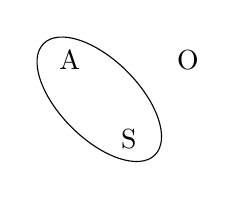
\begin{tikzpicture}
    \node[] at (0,1) {A};
    \node[] at (1.5,1) {O};
    \node[] at (0.75,0) {S};

    \draw[rotate around={45:(0.375,0.5)}] (0.375,0.5) ellipse (0.5 and 1);
  \end{tikzpicture}
  \caption{Nominative-accusative alignment}
  \label{fig:nom-acc-lang}
\end{figure}

In ergative-absolutive languages, the alignment is different. The subject of an intransitive verb (S) has the same marking as the object of the transitive verb (O), namely absolutive. The subject of the transitive verb (A) has its own marking, namely ergative. This is schematically shown in \ref{fig:erg-abs-lang}.

\begin{figure}[ht]
  \centering
  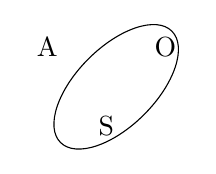
\begin{tikzpicture}
    \node[] at (0,1) {A};
    \node[] at (1.5,1) {O};
    \node[] at (0.75,0) {S};

    \draw[rotate around={135:(0.875,0.5)}] (0.875,0.5) ellipse (0.5 and 1);
  \end{tikzpicture}
  \caption{Ergative-absolutive alignment}
  \label{fig:erg-abs-lang}
\end{figure}

Note here that nominative-accusative languages use the same case marking for the same grammatical function (nominative for subject accusative for object), but ergative-absolutive languages do not.

\citet{bobaljik2006} describes how absolutives and ergatives behave with respect to whether they show agreement. There are languages in which there is agreement with both absolutives and ergatives. Besides that, there are languages in which there is only agreement with absolutives. Crucially, there is no language in which there is only agreement with ergatives. Absolutives are a heterogenous set with respect to grammatical function, i.e. they are subjects of intransitive verbs and objects of transitive verbs. However, with respect to showing agreement absolutives behave the same, and this behaviors is different from ergatives. This indicates that it is morphological case and not grammatical function that is the decisive factor.

\citeauthor{bobaljik2006} (following \citealt{marantz2000}) combines nominative-accusative and ergative-absolutive languages in the following way: accusative and ergative are dependent cases, and nominative or absolutive are unmarked case. Reformulating Figure \ref{fig:agr-sub-do-io} in terms of case instead of grammatical function gives the schema in Figure \ref{fig:agr-nom-acc-dat}.

\begin{figure}[H]
  \centering
  \begin{tikzpicture}
    \draw (0,1) circle (2.25);
    \draw [fill opacity=0.4, fill=LG] (0,0.5) circle (1.75);
    \draw [fill opacity=0.4, fill=DG] (0,0) circle (1.25);

    \node[] at (0,2.75) {unmarked case};
    \node[] at (0,1.5) {dependent case};
    \node[] at (0,0) {dative};

    \node[] at (2.5,3) {\footnotesize{● Japanese}};
    \node[] at (2.25,2) {\footnotesize{● German}};
    \node[] at (2,1) {\footnotesize{● Hungarian}};
    \node[] at (1.375,0) {\footnotesize{● Basque}};
  \end{tikzpicture}
  \caption{\posscitealt{bobaljik2006} actual schema}
  \label{fig:agr-def-dep-dat}
\end{figure}

This formulation in terms of case rather than grammatical function works as follows for the examples I gave earlier.
First, Japanese is a language that does not show any agreement, as shown in \ref{ex:japanese-agr}. There is no agreement with the unmarked case (here the nominative), not with the dependent case (here the accusative) and not with the dative case.
Second, German is a language that shows agreement only with the unmarked case, as shown in \ref{ex:german-agr}. The morpheme \tit{-st} on the predicate agrees with the element in unmarked nominative case \tit{du} `you'. There is no agreement with the dependent accusative case or with the dative case.
Third, Hungarian is a language that shows agreement with the unmarked and the dependent case, as shown in \ref{ex:hungarian-agr}. The portmanteau morpheme \tit{-om} on the predicates agrees with the element in unmarked nominative case \tit{én} `I' and the element in dependent accusative case \tit{a könyvet} `the book'.
Last, Basque is a language that shows agreement with the unmarked, the dependent and the dative case, as shown in \ref{ex:basque-agr}. The morpheme \tit{-zu} on the auxiliary agrees with the element in dependent ergative case \tit{zuk} `you'. The morpheme \tit{d-} on the auxiliary agrees with the element in unmarked absolutive case \tit{liburua} `the book'. The morpheme \tit{-ta} on the auxiliary agrees with the element in dative case \tit{niri} `me'.

In the languages I discuss in this dissertation, I focus on languages that have nominative as unmarked case and accusative as dependent case, so Figure \ref{fig:agr-nom-acc-dat} suffices.

\begin{figure}[ht]
  \centering
  \begin{tikzpicture}
    \draw (0,1) circle (2.25);
    \draw [fill opacity=0.4, fill=LG] (0,0.5) circle (1.75);
    \draw [fill opacity=0.4, fill=DG] (0,0) circle (1.25);

    \node[] at (0,2.75) {\ac{nom}};
    \node[] at (0,1.75) {\ac{acc}};
    \node[] at (0,0) {\ac{dat}};
  \end{tikzpicture}
  \label{fig:agr-nom-acc-dat}
  \caption{\posscitealt{bobaljik2006} simplified schema}
\end{figure}

In sum, this section has shown that agreement follows the same implicational hierarchy as the case scale in headless relatives: \ac{nom} < \ac{acc} < \ac{dat}.


\subsection{Relativization}

Relativization refers to the process in which a relative clause is derived from a non-relative clause. An example of the non-relative clause is given in \ref{ex:rel-non}. The relative clause derived from that is shown in \ref{ex:rel-realati}. The head of the relative clause is \tit{woman} and precedes the clause. The relative pronoun follows the head. The head of the head does not appear in the relative clause anymore.

\ex.
\a. You like the woman. \label{ex:rel-non}
\b. \tbf{the} \tbf{woman}, who you like \label{ex:rel-realati}

In \ref{ex:rel-realati}, it is the object of the clause that is relativized. It differs per language which elements can be relativized with a particular strategy. Just like the distribution was not random for agreement, it is not random which elements can be relativized. Instead, there is an implicational hierarchy that is identical to the one observed for the case scale: \ac{nom} < \ac{acc} < \ac{dat}.

\citet{keenan1977} formulated the implicational hierarchy in terms of the grammatical functions subject, direct object and indirect object.\footnote{
\citet{keenan1977} also included obliques, possessives and objects of comparison on the lowest end of the hierarchy. I leave them out here, because they are not relevant for the discussion.
}
The implicational hierarchy is schematically represented in Figure \ref{fig:rel-sub-do-io}. It should be read as follows: if a language allows a particular relativization strategy of the grammatical function in a particular circle, it also allows this relativization strategy of the grammatical function of the circle around it. The languages in the figure give examples of the circles they are in.

\begin{figure}[ht]
  \centering
  \begin{tikzpicture}
    \draw (0,1) circle (2.25);
    \draw [fill opacity=0.4, fill=LG] (0,0.5) circle (1.75);
    \draw [fill opacity=0.4, fill=DG] (0,0) circle (1.25);

    \node[] at (0,2.75) {subject};
    \node[] at (0,1.5) {direct object};
    \node[align=center] at (0,0) {indirect\\ object};

    \node[] at (2.25,2) {\footnotesize{● Malagasy/German}};
    \node[] at (2,1) {\footnotesize{● Malay}};
    \node[] at (1.375,0) {\footnotesize{● Basque}};
  \end{tikzpicture}
  \caption{Schema for relativization}
  \label{fig:rel-sub-do-io}
\end{figure}

There are four types of languages possible: first, a language that allows only the subject to be relativized with a particular strategy and not the direct and indirect object; second, a language that allows the subject and direct object to be relativized with a particular strategy but not the indirect object; and third, a language that allows the subject, the direct object and the indirect object to be relativized with a particular strategy.

Malagasy is an example of a language that allows subjects to be relativized using a particular strategy, but not direct and indirect objects. \ref{ex:malagasy-decl} is an example of a declarative sentence in Malagasy. It is a transitive sentence that contains the subject \tit{ny mpianatra} `the student' and the direct object \tit{ny vehivavy} `the woman'.

\exg. Nahita ny vehivavy ny mpianatra.\\
 saw the woman the student\\
 `The student saw the woman.' \flushfill{Malagasy, \pgcitealt{keenan1977}{70}}\label{ex:malagasy-decl}

In \ref{ex:malagasy-subj}, the subject from the declarative sentence, marked in bold, is relativized. The subject \tit{ny mpianatra} `the student' appears in the first position of the clause. It is followed by the invariable relativizer \tit{izay} `that'. After that, the rest of the relative clause follows, in this case \tit{nahita ny vehivavy} `saw the woman'.

\exg. \tbf{ny} \tbf{mpianatra} izay nahita ny vehivavy\\
 the student that saw the woman\\
 `the student that saw the woman' \flushfill{Malagasy, \pgcitealt{keenan1977}{70}, my boldfacing}\label{ex:malagasy-subj}

The object of \ref{ex:malagasy-decl} cannot be relativized in the same way, as shown in \ref{ex:malagasy-no-do}. Here the object \tit{ny vehivavy} `the woman', marked in bold, appears in the first position of the clause. It is again followed by the relativizer \tit{izay} `that' and the rest of the relative clause, which is here \tit{nahita ny mpianatra} `saw the student'. This example is ungrammatical.

\exg. *\tbf{ny} \tbf{vehivavy} izay nahita ny mpianatra\\
 the woman that saw the student\\
 `the woman that the student saw' \flushfill{Malagasy, \pgcitealt{keenan1977}{70}, my boldfacing}\label{ex:malagasy-no-do}

Later in this section I draw the parallel between subject and nominative, direct object and accusative and indirect object and dative \citep[after][]{caha2009}. As Malagasy does not have any overt morphological system, it does not hold that the subject corresponds to the nominative in this case.
German is another example of a language that allows subjects to be relativized using a particular strategy, but not direct and indirect object. This strategy is the participle construction \citep{keenan1977}. This strategy is a secondary strategy that exist besides the main strategy that can be used to relativize direct and indirect objects. \ref{ex:german-rel-decl} is an example of a declarative sentence in German. It is a transitive sentence that contains the subject \tit{die Frau} `the woman' and the object \tit{der Mann} `the man'.

\exg. Die Frau küsst den Mann.\\
the woman kisses the man\\
`The woman is kissing the man.' \flushfill{German}\label{ex:german-rel-decl}

The subject from the declarative in \ref{ex:german-rel-decl}, sentence \tit{die Frau} `the woman', is relativized in \ref{ex:german-rel-subj}. The predicate from the declarative clause \tit{küsst} `kisses' is turned in into the participle \tit{küssende} `kissing'. The participle appears at the end of the reduced relative clause \tit{den Mann küssende} `the man kissing'. The reduced relative clause directly precedes the noun of the subject, creating distance between the determiner \tit{die} `the' and \tit{Frau} `woman', which are both marked in bold.

\exg. \tbf{die} den Mann küssende \tbf{Frau}\\
 the the man kissing woman\\
 `the woman who is kissing the man' \flushfill{German}\label{ex:german-rel-subj}

The object from the declarative sentence in \ref{ex:german-rel-decl}, \tit{den Mann} `the man', cannot be relativized like the subject, as shown in \ref{ex:german-rel-no-do}. Again, the predicate from the declarative clause \tit{küsst} `kisses' is turned in into the participle \tit{küssende} `kissing'. The participle appears at the end of the relative clause \tit{die Frau küssende} `the woman kissing'. The reduced relative clause directly precedes the noun of the object, creating distance between the determiner \tit{der} `the' and \tit{Mann} `man', which are both marked in bold. This example is ungrammatical.

\exg. *\tbf{den} die Frau küssende \tbf{Mann}\\
 the the woman kissing man\\
 intended: `the man that the woman is kissing' \flushfill{German}\label{ex:german-rel-no-do}

Malay is an example of a language that has a relativization strategy for subjects and direct objects, but not for indirect objects. \ref{ex:malay-do} shows an example in which the object is relativized. The object here is \tit{ayam} `chicken', marked in bold. It is followed by the relativizer \tit{yang} `that'. After that, the rest of the relative clause \tit{Aminah sedang memakan} `Aminah is eating' follows. The same strategy works to relativize subjects, which is not illustrated with an example.

\exg. Ali bunoh \tbf{ayam} yang Aminah sedang memakan.\\
 Ali kill chicken that Aminah \ac{prog} eat\\
 `Ali killed the chicken that Aminah is eating.' \flushfill{Malay, \pgcitealt{keenan1977}{71}, my boldfacing}\label{ex:malay-do}

Indirect objects cannot be relativized using the same strategy. \ref{ex:malay-decl} is an example of a ditransitive sentence in Malay. The indirect object \tit{kapada perempuan itu} `to the woman' cannot be relativized using \tit{yang}.

\exg. Ali beri {ubi kentang} itu kapada perempuan itu.\\
 Ali give potato the to woman the\\
 `Ali gave the potato to the woman.'\label{ex:malay-decl} \flushfill{Malay, \pgcitealt{keenan1977}{71}}

This is illustrated by the examples in \ref{ex:malay-no-io}. In \ref{ex:malay-no-io1}, the direct object \tit{perempuan kapada} `to the woman', marked in bold, appears in the first position of the clause. It is followed by the relativizer \tit{yang} `that' and the rest of the relative clause \tit{Ali beri ubi kentang itu kapada} `Ali gave the potato to'. This example in ungrammatical.
The example in \ref{ex:malay-no-io2} differs from \ref{ex:malay-no-io1} in that the preposition \tit{kapada} `to' has been moved such that it precedes the relativizer \tit{yang} `that'. This example is ungrammatical as well, indicating this was not the reason for the ungrammaticality.

\ex.\label{ex:malay-no-io}
\ag. *\tbf{perempuan} yang Ali beri {ubi kentang} itu kapada\\
 woman that Ali give potato the to\\\label{ex:malay-no-io1}
\bg. *\tbf{perempuan} \tbf{kapada} yang Ali beri {ubi kentang} itu\\
 woman to who Ali give potato that\\\flushfill{Malay, \pgcitealt{keenan1977}{71}, my boldfacing}\label{ex:malay-no-io2}

% Later in this section I draw the parallel between subject and nominative, direct object and accusative and indirect object and dative \citep[after][]{caha2009}. As Malagasy does not have any overt morphological system, it does not hold that the subject corresponds to the nominative in this case.
% Finnish is another example..
%
%  (12) a. Poydalla tanssinut poika oli sairas.
%  on-table having-danced boy was sick
%  'The boy who had danced on the table was sick.'
%  b. Nakemani poika tanssi poydalla.
%  I-having-seen boy danced on-table
%  'The boy that I saw danced on the table.'



Basque is an example of a language that has a particular relativization strategy for subjects, direct objects and indirect objects. \ref{ex:basque-decl} is an example of a declarative ditransitive sentence in Basque. The sentence contains the subject \tit{gizonak} `the man', the direct object \tit{liburua} `the book' and the indirect object \tit{emakumeari} `the woman'.

\exg. Gizon-a-k emakume-a-ri liburu-a eman dio.\\
 man-\ac{def}-\ac{erg} woman-\ac{def}-\ac{dat} book-\ac{def}.\ac{abs} give has\\
 `The man has given the book to the woman.' \flushfill{Basque, \pgcitealt{keenan1977}{72}}\label{ex:basque-decl}

A relative clause in Basque appears in the prenominal position and it is marked by the invariable marker \tit{-n}.\footnote{
Additionally, the relativized positions do not appear in verbal agreement anymore, but this not visible in the example, because they are all phonologically zero.
}
\ref{ex:basque-sub} shows the three relativizations that are derived from \ref{ex:basque-decl}.
In \ref{ex:basque-sub}, the ergative subject \tit{gizonak} `the man' from \ref{ex:basque-decl} is relativized. The head \tit{gizona} `the man', marked in bold, has lost its ergative marker \tit{-k}, and follows the relative clause \tit{makumeari liburua eman dio} `who has given the book to the woman'. The suffix \tit{-n} is attached to the relative clause.
In \ref{ex:basque-do}, the absolutive direct object \tit{liburua} `the book' from \ref{ex:basque-decl} is relativized. The head \tit{liburua} `the book', marked in bold, follows the relative clause \tit{gizonak emakumeari eman dion} `that the man has given to the woman'.\footnote{
The absolutive direct object \tit{liburua} `the book' does not have an additional overt absolutive marker, so this difference cannot be observed when it is relativized.
}
The suffix \tit{-n} is attached to the relative clause.
In \ref{ex:basque-io}, the dative indirect object \tit{emakumeari} `the woman' from \ref{ex:basque-decl} is relativized. The head \tit{emakumea} `the man', marked in bold, has lost its dative marker \tit{-ri}, and follows the relative clause \tit{gizonak liburua eman dion} `that the man has given the book to'. The suffix \tit{-n} is attached to the relative clause.

\ex.\label{ex:basque-rel}
\ag. emakume-a-ri liburu-a eman dio-n \tbf{gizon-a}\\
 woman-\ac{def}-\ac{dat} book-\ac{def}.\ac{abs} give has-\ac{rel} man-\ac{def}\\
 `the man who has given the book to the woman'\label{ex:basque-sub}
\bg. gizon-a-k emakume-a-ri eman dio-n \tbf{liburu-a}\\
 man-\ac{def}-\ac{erg} woman-\ac{def}-\ac{dat} give has-\ac{rel} book-\ac{def}\\
 `the book that the man has given to the woman'\label{ex:basque-do}
\bg. gizon-a-k liburu-a eman dio-n \tbf{emakume-a}\\
 man-\ac{def}-\ac{erg} book-\ac{def}.\ac{abs} give has-\ac{rel} woman-\ac{def}\\
 `the woman that the man has given the book to' \flushfill{Basque, \pgcitealt{keenan1977}{72}, my boldfacing}\label{ex:basque-io}

\citet{caha2009} argues that the implicational hierarchy is more accurate if it is stated in terms of case rather than grammatical function. The main argument comes from ergative-absolutive languages, which was also one of \posscitet{bobaljik2006} argument with the implicational hierarchy for agreement. \citet{keenan1977} point out that some ergative-absolutive languages form a counterexample to their hierarchy. \citet{caha2009} points out that ergative subjects and oblique noun phrases use the same relativization strategy, which is not allowed with absolutive objects (which is also briefly mentioned in
\citealt{bobaljik2006}).

Reformulating Figure \ref{fig:agr-sub-do-io} in terms of case instead of grammatical function gives the schema in Figure \ref{fig:agr-nom-acc-dat}.

\begin{figure}[ht]
  \centering
  \begin{tikzpicture}
    \draw (0,1) circle (2.25);
    \draw [fill opacity=0.4, fill=LG] (0,0.5) circle (1.75);
    \draw [fill opacity=0.4, fill=DG] (0,0) circle (1.25);

    \node[] at (0,2.75) {unmarked case};
    \node[] at (0,1.5) {dependent case};
    \node[align=center] at (0,0) {dative};

    \node[] at (2.25,2) {\footnotesize{● Malagasy/German}};
    \node[] at (2,1) {\footnotesize{● Malay}};
    \node[] at (1.375,0) {\footnotesize{● Basque}};
  \end{tikzpicture}
  \caption{Schema for relativization}
  \label{fig:rel-def-dep-dat}
\end{figure}

This formulation in terms of case rather than grammatical function works as follows for the examples I gave earlier.

First, German is a language that has a particular relativization strategy for the unmarked case, as shown in \ref{ex:german-rel-subj}. The unmarked nominative case can be relativized with a reduced relative clause, but the dependent accusative case and the dative case cannot.
Second,
Last, Basque is a language that has a particular relativization strategy for unmarked, dependent and dative case, as shown in \ref{ex:basque-rel}. The unmarked ergative, dependent absolutive and dative case can be relativized by extraposing the head, and marking it with the invariable marker \tit{-n}.

In the languages I discuss in this dissertation, I focus on languages that have nominative as unmarked case and accusative as dependent case, so Figure \ref{fig:rel-nom-acc-dat} suffices.

\begin{figure}[ht]
  \centering
  \begin{tikzpicture}
    \draw (0,1) circle (2.25);
    \draw [fill opacity=0.4, fill=LG] (0,0.5) circle (1.75);
    \draw [fill opacity=0.4, fill=DG] (0,0) circle (1.25);

    \node[] at (0,2.75) {nominative};
    \node[] at (0,1.5) {accusative};
    \node[align=center] at (0,0) {dative};
  \end{tikzpicture}
  \caption{Schema for relativization}
  \label{fig:rel-nom-acc-dat}
\end{figure}

In sum, this section has shown that relativization follows the same implicational hierarchy as agreement and as the case scale in headless relatives: \ac{nom} < \ac{acc} < \ac{dat}.


\section{In morphology}\label{sec:case-morphology}

In the two previous sections I showed that the case scale \ac{nom} < \ac{acc} < \ac{dat} can be observed in three syntactic phenomena. First, it shows up in case competition in headless relatives. Second, the case scale forms the basis for the implicational hierarchy observed in agreement across languages. Third, the identical implicational holds for relativization strategies cross-linguistically.

In this section, I show that this same case scale also shows up in morphology. First, syncretism only targets continuous regions on the case scale. Second, several languages show formal containment that mirrors the case scale.


\subsection{Syncretism}

Syncretism refers to the phenomenon whereby two or more different functions are fulfilled by a single form \citep[cf.][]{baerman2002}. In this section I discuss literature that shows that syncretism patterns among nominative, accusative and dative are not random. Instead, they pattern along the case scale \ac{nom} < \ac{acc} < \ac{dat}.

It has widely been observed that syncretism is restricted by the linear sequence \ac{nom} --- \ac{acc} --- \ac{dat} \citep{baerman2005,caha2009,zompi2017} (and see \citealt{mcfadden2018,smith2019} for similar claims concerning root suppletion). That is, if one orders cases in this linear sequence, only contiguous regions in the sequence turn out to be syncretic.
Following that, four possible patterns are attested crosslinguistically. First, all three cases are syncretic. Second, nominative and accusative are syncretic and the dative is not. Third, the accusative and the dative are syncretic and the nominative is not. Fourth, all cases are non-syncretic.

There is one pattern that is not attested crosslinguistically. This pattern does not target continuous regions, but non-contiguous ones: nominative and dative are syncretic and accusative is not. In other words, there is no ABA pattern (in which a form B intervenes between the two identically formed As) \citep{bobaljik2012}.

Table \ref{tbl:syncretisms} shows examples for each of these possible patterns.
I give an example from three distinct forms from Faroese. The second person singular is \tit{tú} `you' for nominative, \tit{teg} `you' for accusative and \tit{tær} `you' for dative \pgcitep{lockwood1977}{70}.
I give an example from a syncretism between nominative, accusative and dative from Dutch. The second person plural pronoun is \tit{jullie} `you.\ac{pl}' is syncretic between nominative, accusative and dative.
I give an example from a syncretism between accusative and dative but not nominative from Icelandic. The first person singular plural is \tit{okkur} `us' is syncretic between accusative and dative. The nominative has a separate form: \tit{við} `we' \pgcitep{einarsson1949}{68}.
I give an example from a syncretism between nominative and accusative but not dative from German. The third person singular feminine \tit{sie} `she/her' is syncretic between nominative and accusative. The dative has a separate form: \tit{ihr} `her'.
Crucially, to the best of my knowledge, there is no language in which the nominative and the dative are syncretic but the accusative is not.

\begin{table}[ht]
  \center
  \caption {}
    % !TEX root = ../thesis.tex

\begin{tabular}{cccccccc}
  \toprule
      \multicolumn{3}{c}{pattern}
        & \ac{nom}
        & \ac{acc}
        & \ac{dat}
        & translation
        & language \\
  \cmidrule(lr){1-3} \cmidrule(lr){4-6} \cmidrule(lr){7-7} \cmidrule(lr){8-8}
      A & A & A
        & \cellcolor{LG}jullie
        & \cellcolor{LG}jullie
        & \cellcolor{LG}jullie
        & 2\ac{pl}
        & Dutch \\
      A & A & B
        & \cellcolor{LG}sie
        & \cellcolor{LG}sie
        & ihr
        & 3\ac{sg}.\ac{f}
        & German \\
      A & B & B
        & við
        & \cellcolor{LG}okkur
        & \cellcolor{LG}okkur
        & 1\ac{pl}
        & Icelandic \\
      A & B & C
        & tú
        & teg
        & tær
        & 2\ac{sg}
        & Faroese \\
      A & B & A
        & \cellcolor{LG}
        &
        & \cellcolor{LG}
        &
        & not attested \\
  \bottomrule
\end{tabular}

  \label{tbl:syncretisms}
\end{table}

In sum, case syncretism follows the ordering of the case scale in headless relatives: \ac{nom} < \ac{acc} < \ac{dat}.


\subsection{Formal containment}

This section shows a second way in which \ac{nom} < \ac{acc} < \ac{dat} is reflected in morphology: formal containment \citep[cf.][]{smith2019,zompi2017,caha2010}. In some languages, the form that is used for the accusative literally contains the form that is used for the nominative. In turn, the forms for the dative contains the form for the accusative. I illustrate this phenomenon with examples from Khanty.

Khanty (or Ostyak) shows formal containment in some of its pronouns (\pgcitealt{nikolaeva1999}{16} after \citealt{smith2019}). Three examples are given in Table \ref{tbl:cont-khanty}.

The nominative form for the first person singular is \tit{ma} `I.\ac{nom}'. The form for the accusative is \tit{ma:ne:m} `me'. This is the form for the nominative \tit{ma} plus the accusative marker \tit{-ne:m}. The form for the dative is \tit{ma:ne:mna} `me'. This is the form for the accusative \tit{ma:ne:m} plus the dative marker \tit{-na}. So, dative formally contains the accusative, and the accusative formally contains the nominative.

The third person singular and first person plural show the same pattern. The accusative forms \tit{luwe:l} `him/her' and \tit{muŋe:w} `us' contain the nominative forms \tit{luw} and the \tit{muŋ} plus the accusative marker \tit{-e:l} or \tit{-e:w}. The dative forms \tit{luwe:lna} `him/her' and \tit{muŋe:wna} `us' contain the accusative forms \tit{luwe:l} and \tit{muŋe:w} plus the dative marker \tit{-na}. Again, the dative formally contains the accusative, which in turn contains the nominative.

\begin{table}[ht]
  \center
  \caption {Case containment in Khanty}
  \begin{tabular}{clll}
  \toprule
            & \ac{1}\ac{sg}
            & \ac{3}\ac{sg}
            & \ac{1}\ac{pl}                           \\
            \cmidrule{2-4}
  \ac{nom}  & ma
            & luw
            & muŋ                                     \\
  \ac{acc}  & ma:\tbf{-ne:m}
            & luw\tbf{-e:l}
            & muŋ\tbf{-e:w}                           \\
  \ac{dat}  & ma:\tbf{-ne:m}\tcol{DG}{\tbf{-na}}
            & luw\tbf{-e:l}\tcol{DG}{\tbf{-na}}
            & muŋ\tbf{-e:w}\tcol{DG}{\tbf{-na}}       \\
  \bottomrule
  \end{tabular}
  \label{tbl:cont-khanty}
\end{table}

Other languages that show this phenomenon are West Tocharian \citep{gippert1987} and Vlakh and Kalderaš Romani (respectively \citealt{friedman1991} and \citealt{boretzky1994}).

In sum, some languages morphologically look like \ac{nom}-\ac{acc}-\ac{dat}. This exactly reflects the case scale \ac{nom} < \ac{acc} < \ac{dat}.

\section{Summary}

Case competition in headless relatives adheres to the case scale in \ref{ex:case-scale-sum}. If the internal and external case differ, cases more on the right of the scale win over cases more to the left on the case.

\ex. \ac{nom} < \ac{acc} < \ac{dat}\label{ex:case-scale-sum}

This case scale is not only found in case competition in headless relatives. Implicational hierarchies regarding two syntactic phenomena appear across languages. The first one concerns agreement. If a language shows agreement with datives, it also shows agreement with accusatives and nominatives. If a language shows agreement with accusatives, it also shows agreement with nominatives.
The second implicational hierarchy concerns relativization. If a dative in a language can be relativized with a particular strategy, an accusative and a nominative can be too using the same strategy. If an accusative can be relativized with a particular strategy, so can a nominative with this strategy.

The case scale also shows up in morphological patterns. First, if the cases are ordered according to the case scale, syncretism only target continuous forms, no ABA pattern appears. Second, some languages show how the dative formally contains accusative, and how the accusative formally contains the nominative.

These phenomena show that the pattern observed in headless relatives is not something that stands on itself. The scale is a pattern that recurs across languages and across different phenomena. Therefore, it should not be treated as an special process with its own stipulated rule. Instead, it is something general that should also follow from general processes in languages.

The next chapter shows how features of the nominative, accusative and dative are organized. All facts presented in this chapter can be derived from the organization of these features.

% % !TEX root = thesis.tex

\chapter{Case decomposition}\label{ch:decomposition}

This chapter provides a theory that derives the first aspect of case competition in headless relatives that I discuss in this dissertation.
This theory seeks to capture that headless relatives crosslinguistically adhere to the case scale \tsc{nom} < \tsc{acc} < \tsc{dat}.

In most existing accounts for case competition in headless relatives (\citealt[cf.][]{pittner1995,vogel2001,grosu2003,harbert1978}, an exception to this is \citealt{himmelreich2017}) the case scale is stipulated. Headless relatives are said to simply obey to that scale. \pgcitet{pittner1995}{fn.4} makes this explicit: ``One of the reviewers notes that an explanation in terms of a Case hierarchy is rather stipulative. However, as far as I know, nobody has suggested a nonstipulative explanation for these facts.''

In the previous chapter I showed that the case scale \ac{nom} < \ac{acc} < \ac{dat} is not specific to headless relatives, but it is a wide-spread phenomenon: it can also be observed in morphology (and in syntax).

Within morphology it appears in syncretism patterns and morphological case containment. \pgcitet{pittner1995}{201:fn.4} makes this link to morphology as well: ``Furthermore, the Case hierarchies receive some independent support by morphology as shown by the various inflectional paradigms.''

As I already eluded to in the summary of Chapter \ref{ch:introduction}, I am not after a theory in which the case scale is something construction-specific, or one in which syntax and morphology both have their own case scale. Instead, argue that there is a single trigger that is responsible for the case scales in different subparts of language (which is identical to what \citealt{caha2019} suggests for case competition in numeral phrases). Specifically, I show that the observed case scale naturally follows on the assumption that the case scale is deeply anchored in syntax. The case scales in morphology and syntax are merely reflexes of how case is organized in the linguistic system.\footnote{
\citet{himmelreich2017} works this intuition out in a different way.
}

This chapter is structured as follows. First, I introduce a specific cumulative case decomposition \citep{caha2009}. In the two following sections, I show how this case decomposition is able to derive the syncretism and morphological case containment facts from Chapter \ref{ch:recurring}. I make this concrete in the framework Nanosyntax \citep{starke2009}. Finally, I show how the case decomposition relates to the winner in case competition in headless relatives.


\section{The basic idea}

\citet{caha2009,caha2013} (followed by \citealt[cf.][]{starke2009,bobaljik2012,mcfadden2018,smith2019,vanbaal2018}) has extensively argued that case should be decomposed into privative features. Specifically, the decomposition is cumulative: each case has a different number of case features, and the number grows one by one.
This is illustrated in Table \ref{tbl:case-decomposed}. Accusative has all the features that nominative has (here \tsc{k}1) plus one extra (here \tsc{k}2). Dative has all the features accusative has (\tsc{k}1 and \tsc{k}2) plus one extra (\tsc{k}3).

\begin{table}[ht]
  \center
	\caption {Cumulative case decomposition}
		\begin{tabular}{ll}
    \toprule
    case      & features                  \\
    \midrule
    \ac{nom} & \tsc{k}1                    \\
    \ac{acc} & \tsc{k}1, \tsc{k}2           \\
    \ac{dat} & \tsc{k}1, \tsc{k}2, \tsc{k}3  \\
    \bottomrule
    \end{tabular}
    \label{tbl:case-decomposed}
\end{table}

Consider the case scale, repeated in repeated in \ref{ex:case-scale-derive}.

\ex. \ac{nom} < \ac{acc} < \ac{dat}\label{ex:case-scale-derive}

This scale actually indicates containment.
Nominative corresponds to a set of features (\tsc{k}1) that is contained in the set of features of accusative (\tsc{k}1 and \tsc{k}2).
Similarly, nominative corresponds to a set of features that is contained in the set of features of dative (\tsc{k}1, \tsc{k}2 and \tsc{k}3).
Lastly, accusative corresponds to a set of features (\tsc{k}1 and \tsc{k}2) that is contained in the set of features of dative (\tsc{k}1, \tsc{k}2 and \tsc{k}3).

The decomposition in Table \ref{tbl:case-decomposed} forms the basis to derive the case scale effects observed in Chapter \ref{ch:recurring}. The following sections show how morphological case containment and syncretism effects follow naturally. After that, I show how the decomposition also derives the case competition facts in headless relatives.


\section{Deriving syncretism}\label{sec:syncretism}

Case syncretism follows the ordering of the case scale. Along this scale, only contiguous regions in the sequence are syncretic. In this section I show how case syncretism patterns can be derived from the case decomposition shown in Table \ref{tbl:case-decomposed}.
In Table \ref{tbl:syncretisms-derive} I repeat the examples that shows the possible and impossible syncretism patterns.

\begin{table}[ht]
  \center
  \caption {Syncretism patterns in Germanic pronouns (repeated)}
    % !TEX root = ../thesis.tex

\begin{tabular}{cccccccc}
  \toprule
      \multicolumn{3}{c}{pattern}
        & \ac{nom}
        & \ac{acc}
        & \ac{dat}
        & translation
        & language \\
  \cmidrule(lr){1-3} \cmidrule(lr){4-6} \cmidrule(lr){7-7} \cmidrule(lr){8-8}
      A & A & A
        & \cellcolor{LG}jullie
        & \cellcolor{LG}jullie
        & \cellcolor{LG}jullie
        & 2\ac{pl}
        & Dutch \\
      A & A & B
        & \cellcolor{LG}sie
        & \cellcolor{LG}sie
        & ihr
        & 3\ac{sg}.\ac{f}
        & German \\
      A & B & B
        & við
        & \cellcolor{LG}okkur
        & \cellcolor{LG}okkur
        & 1\ac{pl}
        & Icelandic \\
      A & B & C
        & tú
        & teg
        & tær
        & 2\ac{sg}
        & Faroese \\
      A & B & A
        & \cellcolor{LG}
        &
        & \cellcolor{LG}
        &
        & not attested \\
  \bottomrule
\end{tabular}

  \label{tbl:syncretisms-derive}
\end{table}

Table \ref{tbl:syncretisms-derive} shows that if one orders cases in the linear sequence \ac{nom} --- \ac{acc} --- \ac{dat}, only contiguous regions in the sequence turn out to be syncretic. First, all three cases can be non-syncretic, as in Faroese. Second, all three cases can be syncretic, as in Dutch. Third, the accusative and the dative can be syncretic and the nominative not, as in Icelandic. Fourth, nominative and accusative can be syncretic and the dative not, as in German. The pattern that is not attested crosslinguistically is the one that targets non-contiguous regions in the table, the ABA pattern \citep{baerman2005,caha2009,zompi2017}.

The syncretism facts follow in a system in which the case is decomposed as in Table \ref{tbl:case-decomposed} and in which lexicalization relies on containment. The latter means that a phonological form is not only inserted when the lexical specification is identical to the syntax, but also when the syntactic features are a subset of the lexical specification. The intuition is the following. Syncretic forms are realized by a single `lexical entry' from the `lexicon'. I elaborate on the terms lexical entry and lexicon shortly.
A lexical entry can be applied if it contains all features, as long as there is no more specific one. This system can generate the patterns ABC, AAA, ABB and AAB, but not ABA.

Before I show how the four attested patterns can be derived (and the unattested one cannot), I need to make some theoretical assumptions explicit about Nanosyntax, the framework in which this dissertation is worked out. First, I show how the Nanosyntactic system is set up in such a way that morphological patterns (like syncretism, but also morphological containment) can inform us about the way syntax is structured. Therefore, I briefly discuss the general architecture of Nanosyntax, its postsyntactic lexicon, and the content and shape of lexical entries. Lastly, I discuss how multiple features (like \tsc{k}1, \tsc{k}2 and \tsc{k}3 from Table \ref{tbl:case-decomposed}) can be spelled out by a single phonological element using phrasal spellout.

In Nanosyntax, syntax starts with atomic features, and it builds complex syntactic trees. Specifically, there are no `feature bundles' (from a pre-syntactic lexicon) that enter the syntax. The only way complex feature structures come to exist is a a result of merge.
After syntax (actually, each instance of merge), the syntactic structure is matched against the lexicon for pronunciation. The lexicon `translates' between lexical trees (i.e. syntactic representations) on the one hand and phonology (PF) and concepts (CF) on the other hand.\footnote{
Throughout the dissertation I call the syntactic representations in the lexicon `lexical trees' in order to distinguish them from syntactic structures in the syntax.
}

In Nanosyntax, the lexicon contains lexical entries, which are links between lexical trees, phonological representations and conceptual representations \citep{starke2014}.\footnote{
The lexical tree does not have to correspond to both a phonological and a conceptual representation. Lexical trees that only correspond to a conceptual representations and not to phonological representations are (phrasal or clausal) idioms. Lexical trees that only correspond to phonological representations but not to conceptual representations are for instance irregular plurals.
} I leave the conceptual representation out of discussion for now, as it is not relevant for the discussion here. The fact that only syntax can create complex feature structures also has a consequence for lexical entries in the lexicon.
Syntactic structures are constrained by certain principles, such that only well-formed syntactic structures exist. Since lexical entries in the lexicon link lexical trees to phonological and conceptual representation, these lexical trees are constrained by the same principles as syntactic structures are.
As a result, the lexicon only contains well-formed lexical trees. The lexicon does not contain unstructured `feature bundles', because they could never be created by syntax.

Following this logic, a feature bundle as in \ref{ex:feature-set} cannot exist. It cannot have entered syntax, because syntax starts with atomic features. It can also not be created by syntax, because complex structures can only be created with merge.

\ex. [ \tsc{k}1, \tsc{k}2, \tsc{k}3 ]\label{ex:feature-set}

Instead, a possible lexical tree looks as in \ref{ex:feature-structure}. The features are merged one by one in a binary structure.

\ex. \begin{forest} boom
  [\ac{dat}P
      [\tsc{k}3]
      [\ac{acc}P
          [\tsc{k}2]
          [\tsc{k}1]
      ]
  ]
\end{forest}\label{ex:feature-structure}

This structure leads to the concept of phrasal spellout: not terminals but multiple syntactic heads (phrases) are realized with a single piece of phonology (i.e. a single morpheme). Applying this to \ref{ex:feature-structure}, not the terminals \tsc{k}1, \tsc{k}2 and \tsc{k}3 receive a realization, but \ac{acc}P and \ac{dat}P are spelled out. A necessary requirement is that these multiple syntactic heads form a constituent. That means that \ac{dat}P cannot be spelled out without \ac{acc}P.

Let me illustrate all of the above with the Faroese pronouns from Table \ref{tbl:syncretisms-derive}. I simplify the situation in two respects. First, I do not show the internal complexity of the pronouns, including person and number features. Instead, I give a triangle, indicating that this is a complex syntactic structure. I refer to is as the person-number phrase it refers to, e.g. 2\ac{sg}P. Second, in this simplified representation I consider the Faroese pronouns to be monomorphemic. I ignore the fact that all three pronouns have the stem \tit{t} with a suffix following it.

The lexical entry for \tit{tú} is given in \ref{ex:faroese-tu-lexicon}. The lexical tree consists of the second person singular pronoun (the 2\ac{sg}P), and \tsc{k}1, making it a \ac{nom}P. The phonological representation that is linked to the lexical tree is \tit{tú}.\footnote{
Throughout the dissertation, I use lexical trees and phonological forms connected by a double arrow (⇔) to refer to a lexical entry.
}

\ex.
\begin{forest} boom
  [\ac{nom}P
      [\tsc{k}1]
      [2\ac{sg}P
          [\phantom{xxx}, roof]
      ]
  ]
  {\draw (.east) node[right]{⇔ \tit{tú}}; }
\end{forest}
\label{ex:faroese-tu-lexicon}

The lexical entry for \tit{teg} is given in \ref{ex:faroese-teg-lexicon}. The lexical tree consists of all the features of the lexical tree in \ref{ex:faroese-tu-lexicon}, plus \tsc{k}2, making it an \ac{acc}P. The linked phonological representation is \tit{teg}.

\ex.
\begin{forest} boom
  [\ac{acc}P
      [\tsc{k}2]
      [\ac{nom}P
          [\tsc{k}1]
          [2\ac{sg}P
              [\phantom{xxx}, roof]
          ]
      ]
  ]
  {\draw (.east) node[right]{⇔ \tit{teg}}; }
\end{forest}
\label{ex:faroese-teg-lexicon}

The lexical entry for \tit{tær} is given in \ref{ex:faroese-taer-lexicon}. The lexical tree consists of all the features of the lexical tree in \ref{ex:faroese-teg-lexicon}, plus \tsc{k}3, making it an \ac{dat}P. The linked phonological representation is \tit{tær}.

\ex.
\begin{forest} boom
  [\ac{dat}P
      [\tsc{k}3]
      [\ac{acc}P
          [\tsc{k}2]
          [\ac{nom}P
              [\tsc{k}1]
              [2\ac{sg}P
                  [\phantom{xxx}, roof]
              ]
          ]
      ]
  ]
  {\draw (.east) node[right]{⇔ \tit{tær}}; }
\end{forest}
\label{ex:faroese-taer-lexicon}

The lexical trees and their phonological counterparts I gave in \ref{ex:faroese-tu-lexicon} to \ref{ex:faroese-taer-lexicon} are lexical entries.
These lexical entries are used to spell out syntactic structures. I give examples of syntactic structures in \ref{ex:faroese-tu-spellout} to \ref{ex:faroese-taer-spellout}.

The lexical tree in \ref{ex:faroese-tu-lexicon} is identical to the syntactic structure in \ref{ex:faroese-tu-spellout}. Therefore, this syntactic structure is spelled out as \tit{tú}.\footnote{
Throughout this dissertation I circle the part of the syntactic structure that corresponds to a particular lexical entry, and I place the corresponding phonology under it.
}

\ex. \begin{forest} boom
[\ac{nom}P,
tikz={
\node[label=below:\tit{tú},
draw,circle,
scale=0.8,
fit to=tree]{};
}
    [\tsc{k}1]
    [2\ac{sg}P
        [\phantom{xxx}, roof]
    ]
]
\end{forest}
\label{ex:faroese-tu-spellout}

The lexical tree in \ref{ex:faroese-teg-lexicon} is identical to the syntactic structure in \ref{ex:faroese-teg-spellout}, and it is spelled out as \tit{teg}.

\ex. \begin{forest} boom
[\ac{acc}P,
tikz={
\node[label=below:\tit{teg},
draw,circle,
scale=0.825,
fit to=tree]{};
}
    [\tsc{k}2]
    [\ac{nom}P
        [\tsc{k}1]
        [2\ac{sg}P
            [\phantom{xxx}, roof]
        ]
    ]
]
\end{forest}
\label{ex:faroese-teg-spellout}

The lexical tree in \ref{ex:faroese-taer-lexicon} is identical to the syntactic structure in \ref{ex:faroese-taer-spellout}, and it is spelled out as \tit{tær}.

\ex. \begin{forest} boom
[\ac{dat}P,
tikz={
\node[label=below:\tit{tær},
draw,circle,
scale=0.85,
fit to=tree]{};
}
    [\tsc{k}3]
    [\ac{acc}P
        [\tsc{k}2]
        [\ac{nom}P
            [\tsc{k}1]
            [2\ac{sg}P
                [\phantom{xxx}, roof]
            ]
        ]
    ]
]
\end{forest}
\label{ex:faroese-taer-spellout}

In the Faroese examples above, the syntactic structures are all identical to the lexical trees. However, Nanosyntax assumes that to be a successful match, identity is not a necessary requirement. Instead, matching relies on a containment relation. This is formalized as in \ref{ex:superset-principle}.

\ex. \tbf{The Superset Principle} \citet{starke2009}:\\
A lexically stored tree matches a syntactic node iff the lexically stored tree contains the syntactic node.
\label{ex:superset-principle}

Let me illustrate this with the Dutch second person plural pronoun from Table \ref{tbl:syncretisms-derive}. This pronoun is syncretic between between the nominative, accusative and dative.
The lexicon only contains a single lexical entry, namely \ref{ex:dutch-jullie-lexicon}. The lexical tree consists of the complex lexical tree that corresponds to the second person plural pronoun (the \ac{2}\ac{pl}P), and \tsc{k}1, \tsc{k}2 and \tsc{k}3 making it a \ac{dat}P. The phonological representation that is linked to the lexical tree is \tit{jullie}.
The nominative, the accusative and the dative can all be spelled out with this single lexical entry using the Superset Principle in \ref{ex:superset-principle}.

\ex.
\begin{forest} boom
  [\ac{dat}P
      [\tsc{k}3]
      [\ac{acc}P
          [\tsc{k}2]
          [\ac{nom}P
              [\tsc{k}1]
              [2\ac{pl}P
                  [\phantom{xxx}, roof]
              ]
          ]
      ]
  ]
  {\draw (.east) node[right]{⇔ \tit{jullie}}; }
\end{forest}
\label{ex:dutch-jullie-lexicon}

The syntactic structure of the dative, given in \ref{ex:dutch-jullie-spellout-dat}, is the least exciting of the three. It is identical to the lexical tree \ref{ex:dutch-jullie-lexicon}, and therefore, spelled out as \tit{jullie}.

\ex. \begin{forest} boom
[\ac{dat}P,
tikz={
\node[label=below:\tit{jullie},
draw,circle,
scale=0.85,
fit to=tree]{};
}
    [\tsc{k}3]
    [\ac{acc}P
        [\tsc{k}2]
        [\ac{nom}P
            [\tsc{k}1]
            [2\ac{pl}P
                [\phantom{xxx}, roof]
            ]
        ]
    ]
]
\end{forest}
\label{ex:dutch-jullie-spellout-dat}

The syntactic structure of the accusative is given in \ref{ex:dutch-jullie-spellout-acc-empty}.

\ex. \begin{forest} boom
[\ac{acc}P
    [\tsc{k}2]
    [\ac{nom}P
        [\tsc{k}1]
        [2\ac{pl}P
            [\phantom{xxx}, roof]
        ]
    ]
]
\end{forest}
\label{ex:dutch-jullie-spellout-acc-empty}

The lexical entry in \ref{ex:dutch-jullie-lexicon} is not identical to this syntactic structure. However, the lexical tree contains the syntactic structure of the accusative.
I repeat the lexical entry for \tit{jullie} in \ref{ex:dutch-jullie-lexicon-acc}, marking the subpart of the tree that matches the syntactic structure in gray.

\ex. \begin{forest} boom
  [\ac{dat}P
      [\tsc{k}3]
      [\ac{acc}P,
      tikz={
      \node[draw,circle,transparent,
      fill=DG,fill opacity=0.2,
      scale=0.825,
      fit to=tree]{};
      }
          [\tsc{k}2]
          [\ac{nom}P
              [\tsc{k}1]
              [2\ac{pl}P
                  [\phantom{xxx}, roof]
              ]
          ]
      ]
  ]
  {\draw (.east) node[right]{⇔ \tit{jullie}}; }
\end{forest}
\label{ex:dutch-jullie-lexicon-acc}

As a result, the accusative is spelled out as \tit{jullie}, shown in \ref{ex:dutch-jullie-spellout-acc}.

\ex. \begin{forest} boom
[\ac{acc}P,
tikz={
\node[label=below:\tit{jullie},
draw,circle,
scale=0.825,
fit to=tree]{};
}
    [\tsc{k}2]
    [\ac{nom}P
        [\tsc{k}1]
        [2\ac{pl}P
            [\phantom{xxx}, roof]
        ]
    ]
]
\end{forest}
\label{ex:dutch-jullie-spellout-acc}

The same holds for the nominative. The syntactic structure is given in \ref{ex:dutch-jullie-spellout-nom-empty}.

\ex.
\begin{forest} boom
[\ac{nom}P
    [\tsc{k}1]
    [2\ac{pl}P
        [\phantom{xxx}, roof]
    ]
]
\end{forest}
 \label{ex:dutch-jullie-spellout-nom-empty}

The lexical tree in \ref{ex:dutch-jullie-lexicon} is not identical to this syntactic structure. However, again, the lexical tree contains the syntactic structure of the nominative.
I repeat the lexical entry for \tit{jullie} in \ref{ex:dutch-jullie-lexicon-nom}, marking the subpart of the tree that matches the syntactic structure in gray.

 \ex. \begin{forest} boom
   [\ac{dat}P
       [\tsc{k}3]
       [\ac{acc}P
           [\tsc{k}2]
           [\ac{nom}P,
           tikz={
           \node[draw,circle,transparent,
           fill=DG,fill opacity=0.2,
           scale=0.8,
           fit to=tree]{};
           }
               [\tsc{k}1]
               [2\ac{pl}P
                   [\phantom{xxx}, roof]
               ]
           ]
       ]
   ]
   {\draw (.east) node[right]{⇔ \tit{jullie}}; }
 \end{forest}
 \label{ex:dutch-jullie-lexicon-nom}

As a result, the nominative is spelled out as \tit{jullie}, as shown in \ref{ex:dutch-jullie-spellout-nom}.

\ex.
\begin{forest} boom
[\ac{nom}P,
tikz={
\node[label=below:\tit{jullie},
draw,circle,
scale=0.8,
fit to=tree]{};
}
    [\tsc{k}1]
    [2\ac{pl}P
        [\phantom{xxx}, roof]
    ]
]
\end{forest}
 \label{ex:dutch-jullie-spellout-nom}

A question arises at this point. Why are the accusative and nominative in Faroese not spelled out by the lexical entry for the dative (and why is the nominative not spelled out by the lexical entry for the accusative)? These syntactic structures are namely contained in the lexical tree for the dative (and the accusative).
The reason for this comes from how competition between lexical entries is regulated in Nanosyntax. When two lexical entries compete, the best fit wins. The best fit is the lexical tree with the least features that are not used. This is formalized as in \ref{ex:elsewhere-condition}.

\ex. \tbf{The Elsewhere Condition} (\citealt{kiparsky1973}, formulated as in \citealt{caha2020}):\\
When two entries can spell out a given node, the more specific entry wins. Under the Superset Principle governed insertion, the more specific entry is the one which has fewer unused features.
\label{ex:elsewhere-condition}

I show how the Superset Principle and the Elsewhere Condition interact in a competition with the Faroese lexical entries I discussed earlier in this section. I only discuss the nominative \tit{tú} and the accusative \tit{teg}, because for the dative \tit{tær} there is only a single candidate that contains all features: the lexical entry \tit{tær}.

Consider first again the syntactic structure for the nominative in \ref{ex:faroese-tu-structure-nom}, repeated from \ref{ex:faroese-tu-spellout}.

\ex. \begin{forest} boom
[\ac{nom}P
    [\tsc{k}1]
    [2\ac{sg}P
        [\phantom{xxx}, roof]
    ]
]
\end{forest}
\label{ex:faroese-tu-structure-nom}

The three lexical entries for \tit{tú}, \tit{teg} and \tit{tær} are candidates for this syntactic structure.
I repeat them in \ref{ex:faroese-lexicon-nom}, marking the subpart of the tree that matches the syntactic structure in gray.

\ex.\label{ex:faroese-lexicon-nom}
\a.
\begin{forest} boom
  [\ac{nom}P,
  tikz={
  \node[draw,circle,transparent,
  fill=DG,fill opacity=0.2,
  scale=0.8,
  fit to=tree]{};
  }
    [\tsc{k}1]
      [2\ac{sg}P
          [\phantom{xxx}, roof]
      ]
  ]
  {\draw (.east) node[right]{⇔ \tit{tú}}; }
\end{forest}
\label{ex:faroese-tu-lexicon-nom}
\b.
\begin{forest} boom
  [\ac{acc}P
      [\tsc{k}2]
      [\ac{nom}P,
      tikz={
      \node[draw,circle,transparent,
      fill=DG,fill opacity=0.2,
      scale=0.8,
      fit to=tree]{};
      }
          [\tsc{k}1]
          [2\ac{sg}P
              [\phantom{xxx}, roof]
          ]
      ]
  ]
  {\draw (.east) node[right]{⇔ \tit{teg}}; }
\end{forest}
\label{ex:faroese-teg-lexicon-nom}
\b. \begin{forest} boom
  [\ac{dat}P
      [\tsc{k}3]
      [\ac{acc}P
          [\tsc{k}2]
          [\ac{nom}P,
          tikz={
          \node[draw,circle,transparent,
          fill=DG,fill opacity=0.2,
          scale=0.8,
          fit to=tree]{};
          }
              [\tsc{k}1]
              [2\ac{sg}P
                  [\phantom{xxx}, roof]
              ]
          ]
      ]
  ]
  {\draw (.east) node[right]{⇔ \tit{tær}}; }
\end{forest}
\label{ex:faroese-taer-lexicon-nom}

The first, \ref{ex:faroese-tu-lexicon-nom}, has no unused features. The second, \ref{ex:faroese-teg-lexicon-nom}, has one unused feature: \tsc{k}2. The third, \ref{ex:faroese-taer-lexicon-nom}, has two unused features: \tsc{k}2 and \tsc{k}3.
Because \ref{ex:faroese-tu-lexicon-nom} has the least amount of unused features, it wins the competition, and the syntactic structure is spelled out as \tit{tú}. This is shown in \ref{ex:faroese-tu-spellout-nom}.

\ex. \begin{forest} boom
[\ac{nom}P,
tikz={
\node[label=below:\tit{tú},
draw,circle,
scale=0.8,
fit to=tree]{};
}
    [\tsc{k}1]
    [2\ac{sg}P
        [\phantom{xxx}, roof]
    ]
]
\end{forest}
\label{ex:faroese-tu-spellout-nom}

Consider the syntactic structure for the accusative in \ref{ex:faroese-teg-structure}, repeated from \ref{ex:faroese-teg-spellout}.

\ex. \begin{forest} boom
[\ac{acc}P
    [\tsc{k}2]
    [\ac{nom}P
        [\tsc{k}1]
        [2\ac{sg}P
            [\phantom{xxx}, roof]
        ]
    ]
]
\end{forest}
\label{ex:faroese-teg-structure}

The two lexical entries for \tit{teg} and \tit{tær} are candidates for this syntactic structure. The lexical entry for \tit{tú} is not a candidate here, because it does not contain the complete syntactic structure (i.e. it lacks \tsc{k}2).
I repeat the lexical entries for \tit{teg} and \tit{tær} in \ref{ex:faroese-lexicon-acc}, marking the subpart of the tree that matches the syntactic structure in gray.

\ex.\label{ex:faroese-lexicon-acc}
\a.
\begin{forest} boom
  [\ac{acc}P,
  tikz={
  \node[draw,circle,transparent,
  fill=DG,fill opacity=0.2,
  scale=0.825,
  fit to=tree]{};
  }
      [\tsc{k}2]
      [\ac{nom}P
          [\tsc{k}1]
          [2\ac{sg}P
              [\phantom{xxx}, roof]
          ]
      ]
  ]
  {\draw (.east) node[right]{⇔ \tit{teg}}; }
\end{forest}
\label{ex:faroese-teg-lexicon-acc}
\b.
\begin{forest} boom
  [\ac{dat}P
      [\tsc{k}3]
      [\ac{acc}P,
      tikz={
      \node[draw,circle,transparent,
      fill=DG,fill opacity=0.2,
      scale=0.825,
      fit to=tree]{};
      }
          [\tsc{k}2]
          [\ac{nom}P
              [\tsc{k}1]
              [2\ac{sg}P
                  [\phantom{xxx}, roof]
              ]
          ]
      ]
  ]
  {\draw (.east) node[right]{⇔ \tit{tær}}; }
\end{forest}
\label{ex:faroese-taer-lexicon-acc}

The former, \ref{ex:faroese-teg-lexicon-acc}, has no unused features. The latter, \ref{ex:faroese-taer-lexicon-acc}, has one unused feature: \tsc{k}2.
Because \ref{ex:faroese-teg-lexicon-acc} has fewer unused features than \ref{ex:faroese-taer-lexicon-acc}, it wins the competition, and the syntactic structure is spelled out as \tit{teg}. This is shown in \ref{ex:faroese-teg-spellout-acc}.

\ex. \begin{forest} boom
[\ac{acc}P,
tikz={
\node[label=below:\tit{teg},
draw,circle,
scale=0.825,
fit to=tree]{};
}
    [\tsc{k}2]
    [\ac{nom}P
        [\tsc{k}1]
        [2\ac{sg}P
            [\phantom{xxx}, roof]
        ]
    ]
]
\end{forest}
\label{ex:faroese-teg-spellout-acc}

Table \ref{tbl:syncretisms-derive} contains two more attested patterns: the ABB pattern in Icelandic and the AAB pattern in German. In the remainder of this section I show how these two patterns are derived. I also show how the system is unable to derive an ABA pattern, which is crosslinguistically unattested \citep{baerman2005,caha2009,zompi2017}.

Consider the Icelandic pattern. For the first person plural, Icelandic uses \tit{við} as nominative and \tit{okkur} as accusative and dative. Two lexical entries are needed for this. The first one in \ref{ex:icelandic-vid-lexicon} contains pronominal features and \tsc{k}1, and corresponds to the phonology \tit{við}.
The second one is given in \ref{ex:icelandic-okkur-lexicon}. It contains in addition to \ref{ex:icelandic-vid-lexicon} also the feature \tsc{k}2 and \tsc{k}3. The phonological representation that is linked to it is \tit{okkur}.

\ex.
\a.
\begin{forest} boom
  [\ac{nom}P
      [\tsc{k}1]
      [1\ac{pl}P
          [\phantom{xxx}, roof]
      ]
  ]
  {\draw (.east) node[right]{⇔ \tit{við}}; }
\end{forest}
\label{ex:icelandic-vid-lexicon}
\b.
\begin{forest} boom
  [\ac{dat}P
      [\tsc{k}3]
      [\ac{acc}P
          [\tsc{k}2]
          [\ac{nom}P
              [\tsc{k}1]
              [\ac{1}\ac{pl}P
                  [\phantom{xxx}, roof]
              ]
          ]
      ]
  ]
  {\draw (.east) node[right]{⇔ \tit{okkur}}; }
\end{forest}
\label{ex:icelandic-okkur-lexicon}

The syntactic structure for the dative is given in \ref{ex:icelandic-okkur-spellout-dat}. It is contained in the lexical tree in \ref{ex:icelandic-okkur-lexicon}, and therefore, spelled out as \tit{okkur}.
The lexical entry in \ref{ex:icelandic-vid-lexicon} is not considered, because it does not contain \tsc{k}2 and \tsc{k}3.

\ex. \begin{forest} boom
[\ac{dat}P,
tikz={
\node[label=below:\tit{okkur},
draw,circle,
scale=0.85,
fit to=tree]{};
}
    [\tsc{k}3]
    [\ac{acc}P
        [\tsc{k}2]
        [\ac{nom}P
            [\tsc{k}1]
            [1\ac{pl}P
                [\phantom{xxx}, roof]
            ]
        ]
    ]
]
\end{forest}
\label{ex:icelandic-okkur-spellout-dat}

The syntactic structure for the accusative is given in \ref{ex:icelandic-okkur-spellout-acc}. It is contained in the lexical tree in \ref{ex:icelandic-okkur-lexicon}, and therefore, spelled out as \tit{okkur}.
The lexical entry in \ref{ex:icelandic-vid-lexicon} is not considered, because it does not contain \tsc{k}2.

\ex. \begin{forest} boom
[\ac{acc}P,
tikz={
\node[label=below:\tit{okkur},
draw,circle,
scale=0.825,
fit to=tree]{};
}
    [\tsc{k}2]
    [\ac{nom}P
        [\tsc{k}1]
        [1\ac{pl}P
            [\phantom{xxx}, roof]
        ]
    ]
]
\end{forest}
\label{ex:icelandic-okkur-spellout-acc}

The syntactic structure for the nominative is given in \ref{ex:icelandic-vid-structure}.

\ex. \begin{forest} boom
[\ac{nom}P
    [\tsc{k}1]
    [1\ac{pl}P
        [\phantom{xxx}, roof]
    ]
]
\end{forest}
\label{ex:icelandic-vid-structure}

It is contained in the lexical tree for \tit{við} and in the one for \tit{okkur}.
I repeat the lexical entries for \tit{við} and \tit{okkur} in \ref{icelandic-lexicon-nom}, marking the subparts of the trees that match the syntactic structure in gray.

\ex.\label{icelandic-lexicon-nom}
\a.
\begin{forest} boom
  [\ac{nom}P,
  tikz={
  \node[draw,circle,transparent,
  fill=DG,fill opacity=0.2,
  scale=0.8,
  fit to=tree]{};
  }
      [\tsc{k}1]
      [1\ac{pl}P
          [\phantom{xxx}, roof]
      ]
  ]
  {\draw (.east) node[right]{⇔ \tit{við}}; }
\end{forest}
\label{ex:icelandic-vid-lexicon-nom}
\b.
\begin{forest} boom
  [\ac{dat}P
      [\tsc{k}3]
      [\ac{acc}P
          [\tsc{k}2]
          [\ac{nom}P,
          tikz={
          \node[draw,circle,transparent,
          fill=DG,fill opacity=0.2,
          scale=0.8,
          fit to=tree]{};
          }
              [\tsc{k}1]
              [1\ac{pl}P
                  [\phantom{xxx}, roof]
              ]
          ]
      ]
  ]
  {\draw (.east) node[right]{⇔ \tit{okkur}}; }
\end{forest}
\label{ex:icelandic-okkur-lexicon-nom}

The former, \ref{ex:icelandic-vid-lexicon-nom}, has no unused features. The latter, \ref{ex:icelandic-okkur-lexicon-nom}, has two unused features: \tsc{k}2 and \tsc{k}3.
Because \ref{ex:icelandic-vid-lexicon-nom} has fewer unused features, it wins the competition, and the syntactic structure is spelled out as \tit{við}. This is shown in \ref{ex:icelandic-vid-spellout-nom}.

\ex. \begin{forest} boom
[\ac{nom}P,
tikz={
\node[label=below:\tit{við},
draw,circle,
scale=0.8,
fit to=tree]{};
}
    [\tsc{k}1]
    [1\ac{pl}P
        [\phantom{xxx}, roof]
    ]
]
\end{forest}
\label{ex:icelandic-vid-spellout-nom}

For the third person singular feminine, German uses \tit{sie} as nominative and accusative, and \tit{ihr} as dative. Two lexical entries are needed for this.
The first one in \ref{ex:german-sie-lexicon} contains pronominal features, \tsc{k}1 and \tsc{k}2. It corresponds to the phonology \tit{sie}.
The second one is given in \ref{ex:german-ihr-lexicon}. It contains in addition to \tit{sie} in \ref{ex:german-sie-lexicon} also the feature \tsc{k}3. It corresponds to the phonology \tit{ihr}.

\ex.
\a.
\begin{forest} boom
  [\ac{acc}P
      [\tsc{k}2]
      [\ac{nom}P
          [\tsc{k}1]
          [\ac{3}\ac{sg}.\tsc{k}P
              [\phantom{xxx}, roof]
          ]
      ]
  ]
  {\draw (.east) node[right]{⇔ \tit{sie}}; }
\end{forest}
\label{ex:german-sie-lexicon}
\b.
\begin{forest} boom
  [\ac{dat}P
      [\tsc{k}3]
      [\ac{acc}P
          [\tsc{k}2]
          [\ac{nom}P
              [\tsc{k}1]
              [3\ac{sg}.\tsc{k}P
                  [\phantom{xxx}, roof]
              ]
          ]
      ]
  ]
  {\draw (.east) node[right]{⇔ \tit{ihr}}; }
\end{forest}
\label{ex:german-ihr-lexicon}

The syntactic structure for the dative is given in \ref{ex:german-ihr-spellout}. It is contained in the lexical tree in \ref{ex:german-ihr-lexicon}, and therefore, spelled out as \tit{ihr}.
The lexical entry in \ref{ex:german-sie-lexicon} is not considered, because it does not contain \tsc{k}3.

\ex. \begin{forest} boom
[\ac{dat}P,
tikz={
\node[label=below:\tit{ihr},
draw,circle,
scale=0.85,
fit to=tree]{};
}
    [\tsc{k}3]
    [\ac{acc}P
        [\tsc{k}2]
        [\ac{nom}P
            [\tsc{k}1]
            [3\ac{sg}.\tsc{k}P
                [\phantom{xxx}, roof]
            ]
        ]
    ]
]
\end{forest}
\label{ex:german-ihr-spellout}

The syntactic structure for the accusative is given in \ref{ex:german-sie-structure-acc}.

\ex. \begin{forest} boom
[\ac{acc}P
    [\tsc{k}2]
    [\ac{nom}P
        [\tsc{k}1]
        [3\ac{sg}.\tsc{k}P
            [\phantom{xxx}, roof]
        ]
    ]
]
\end{forest}
\label{ex:german-sie-structure-acc}

It is contained in the lexical tree for \tit{sie} and in the one for \tit{ihr}.
I repeat the lexical entries for \tit{sie} and \tit{ihr} in \ref{ex:german-lexicon-acc}, marking the subparts of the trees that match the syntactic structure in gray.

\ex.\label{ex:german-lexicon-acc}
\a.
\begin{forest} boom
  [\ac{acc}P,
  tikz={
  \node[draw,circle,transparent,
  fill=DG,fill opacity=0.2,
  scale=0.825,
  fit to=tree]{};
  }
      [\tsc{k}2]
      [\ac{nom}P
          [\tsc{k}1]
          [3\ac{sg}.\tsc{k}P
              [\phantom{xxx}, roof]
          ]
      ]
  ]
  {\draw (.east) node[right]{⇔ \tit{sie}}; }
\end{forest}
\label{ex:german-sie-lexicon-acc}
\b.
\begin{forest} boom
  [\ac{dat}P
      [\tsc{k}3]
      [\ac{acc}P,
      tikz={
      \node[draw,circle,transparent,
      fill=DG,fill opacity=0.2,
      scale=0.825,
      fit to=tree]{};
      }
          [\tsc{k}2]
          [\ac{nom}P
              [\tsc{k}1]
              [3\ac{sg}.\tsc{k}P
                  [\phantom{xxx}, roof]
              ]
          ]
      ]
  ]
  {\draw (.east) node[right]{⇔ \tit{ihr}}; }
\end{forest}
\label{ex:german-ihr-lexicon-acc}

The former, \ref{ex:german-sie-lexicon-acc}, has one no unused features. The latter, \ref{ex:german-ihr-lexicon-acc}, has one unused feature: \tsc{k}3.
Because \ref{ex:german-sie-lexicon-acc} has fewer unused features, it wins the competition, and the syntactic structure is spelled out as \tit{sie}. This is shown in \ref{ex:german-sie-spellout-acc}

\ex. \begin{forest} boom
[\ac{acc}P,
tikz={
\node[label=below:\tit{sie},
draw,circle,
scale=0.825,
fit to=tree]{};
}
    [\tsc{k}2]
    [\ac{nom}P
        [\tsc{k}1]
        [3\ac{sg}.\tsc{k}P
            [\phantom{xxx}, roof]
        ]
    ]
]
\end{forest}
\label{ex:german-sie-spellout-acc}

The syntactic structure for the nominative is given in \ref{ex:german-sie-structure}.

\ex. \begin{forest} boom
[\ac{nom}P
    [\tsc{k}1]
    [3\ac{sg}.\tsc{k}P
        [\phantom{xxx}, roof]
    ]
]
\end{forest}
\label{ex:german-sie-structure}

It is contained in the lexical tree for \tit{sie} and in the one \tit{ihr}.
I repeat the lexical entries for \tit{sie} and \tit{ihr} in \ref{ex:german-lexicon-nom}, marking the subparts of the trees that match the syntactic structure in gray.

\ex.\label{ex:german-lexicon-nom}
\a.
\begin{forest} boom
  [\ac{acc}P
      [\tsc{k}2]
      [\ac{nom}P,
      tikz={
      \node[draw,circle,transparent,
      fill=DG,fill opacity=0.2,
      scale=0.8,
      fit to=tree]{};
      }
          [\tsc{k}1]
          [3\ac{sg}.\tsc{k}P
              [\phantom{xxx}, roof]
          ]
      ]
  ]
  {\draw (.east) node[right]{⇔ \tit{sie}}; }
\end{forest}
\label{ex:german-sie-lexicon-nom}
\b.
\begin{forest} boom
  [\ac{dat}P
      [\tsc{k}3]
      [\ac{acc}P
          [\tsc{k}2]
          [\ac{nom}P,
          tikz={
          \node[draw,circle,transparent,
          fill=DG,fill opacity=0.2,
          scale=0.8,
          fit to=tree]{};
          }
              [\tsc{k}1]
              [3\ac{sg}.\tsc{k}P
                  [\phantom{xxx}, roof]
              ]
          ]
      ]
  ]
  {\draw (.east) node[right]{⇔ \tit{ihr}}; }
\end{forest}
\label{ex:german-ihr-lexicon-nom}

The former, \ref{ex:german-sie-lexicon-nom}, has one unused feature: \tsc{k}2. The latter, \ref{ex:german-ihr-lexicon-nom}, has two unused features: \tsc{k}2 and \tsc{k}3.
Because \ref{ex:german-sie-lexicon-nom} has fewer unused features, it wins the competition, and the syntactic structure is spelled out as \tit{sie}. This is shown in \ref{ex:german-sie-spellout-nom}.

\ex. \begin{forest} boom
[\ac{nom}P,
tikz={
\node[label=below:\tit{sie},
draw,circle,
scale=0.8,
fit to=tree]{};
}
    [\tsc{k}1]
    [3\ac{sg}.\tsc{k}P
        [\phantom{xxx}, roof]
    ]
]
\end{forest}
\label{ex:german-sie-spellout-nom}

This last example also illustrates that the laid out system is unable to derive an ABA pattern. The unability of the system to derive such a pattern is a welcome one, since the pattern is unattested crosslinguistically. In an ABA pattern, the nominative and the dative are syncretic, to the exclusion of the accusative. Such a language would be like German but then the nominative would be \tit{ihr} instead of \tit{sie}.

This result could never be derived with the lexical entries given in \ref{ex:german-sie-lexicon} and \ref{ex:german-ihr-lexicon}. \tit{Ihr} is inserted for the dative and the cases contained in it (so for accusative and nominative), unless a more specific lexical entry is found. \tit{Sie} is the more specific lexical entry that is found from the accusative on. From the accusative on (so for the accusative and nominative), \tit{sie} will be inserted until a more specific entry is found. If no entry is specified for nominative, \tit{sie} will surface. \tit{Ihr} will not resurface, because the lexical entry for \tit{sie} is and will remain to be more specific.

In sum, the cumulative case decomposition from Table \ref{tbl:case-decomposed} can derive the observed syncretism patterns.

\section{Deriving morphological case containment}

Some languages morphologically reflect the case scale \ac{nom} < \ac{acc} < \ac{dat}. Khanty is an example of such a language. The phonological form of the accusative literally contains the phonological form of the nominative, and the form of the dative contains the form of the accusative. In this section I show how morphological case containment can be derived from the case decomposition in Table \ref{tbl:case-decomposed}. I repeat an example from Khanty that shows morphological case containment in Table \ref{tbl:cont-khanty-3sg} \pgcitep{nikolaeva1999}{16}.

\begin{table}[ht]
  \center
  \caption {Morphological case containment of 3\ac{sg} in Khanty}
    % !TEX root = ../thesis.tex

\begin{tabular}{cl}
\toprule
          & 3\ac{sg} \\
          \cmidrule{2-2}
\ac{nom}
          & luw                                     \\
\ac{acc}  & luw\tbf{-e:l}                           \\
\ac{dat}  & luw\tbf{-e:l}\tcol{DG}{\tbf{-na}}       \\
\bottomrule
\end{tabular}

  \label{tbl:cont-khanty-3sg}
\end{table}

The intuition is the following. The morphological form of the pronouns mirrors the cumulative feature decomposition given in Table \ref{tbl:case-decomposed}. That is, the accusative has the morphology that the nominative has (\tit{luw}) plus something extra (\tit{e:l}). Similarly, the accusative also has the features that the nominative has (\tsc{k}1) plus something extra (\tsc{k}2). The dative has the morphology that the accusative has (\tit{luw-e:l}) plus something extra (\tit{na}). Again, similarly, the dative has the features that the accusative has (\tsc{k}1, \tsc{k}2) plus something extra (\tsc{k}3).

Before I show how languages with morphological case containment can be derived, I need to discuss how variation between languages is modeled in Nanosyntax. Crosslinguistic variation is namely explained in terms of differences in the lexicon. In other words, the syntactic structure is identical across languages, but the lexical entries package features together differently.

Let me discuss the differences between synthetic and agglutinative morphology to make this more concrete. Take the accusative, which contains \tsc{k}1 and \tsc{k}2 in all languages. The languages discussed in the previous section, Section \ref{sec:syncretism}, are all synthetic languages. \tsc{k}2 can only be spelled out in a single lexical entry together with \tsc{k}1. The result is that the examples are syncretic (i.e. formally identical) or suppletive (i.e. formally unrelated). The language I discuss in this section is agglutinative. \tsc{k}2 is not spelled out in the same lexical entry with \tsc{k}1. Instead, the \tsc{k}2 is spelled out by its own lexical entry. The result is that the accusative formally contains the nominative.

Let me illustrate this by deriving the 3\ac{sg} paradigm in Khanty.
First, I give the lexical entry for the nominative third person singular. It contains pronominal features and the feature \tsc{k}1. The phonological form associated with the structure is \tit{luw}. The lexical entry is given in \ref{ex:khanty-luw-lexicon}.

\ex.
\begin{forest} boom
  [\ac{nom}P
      [\tsc{k}1]
      [3\ac{sg}P
          [\phantom{xxx}, roof]
      ]
  ]
  {\draw (.east) node[right]{⇔ \tit{luw}}; }
\end{forest}\label{ex:khanty-luw-lexicon}

The syntactic structure in for the nominative is given in \ref{ex:khanty-luw-spellout}. It is contained in the lexical tree in \ref{ex:khanty-luw-spellout}, and the nominative is spelled out as \tit{luw}.

\ex. \begin{forest} boom
[\ac{nom}P,
tikz={
\node[label=below:\tit{luw},
draw,circle,
scale=0.8,
fit to=tree]{};
}
    [\tsc{k}1]
    [3\ac{sg}P
        [\phantom{xxx}, roof]
    ]
]
\end{forest}\label{ex:khanty-luw-spellout}

As shown in Table \ref{tbl:cont-khanty-3sg}, the morphological form of the accusative contains the morphological form of the nominative \tit{luw} plus an extra morpheme \tit{e:l}. As shown in Table \ref{tbl:case-decomposed}, the syntactic features of the accusative contain the syntactic features of the nominative \tsc{k}1 plus an extra feature \tsc{k}2.
Accordingly, I give the lexical entry for the accusative marker \tit{e:l} in \ref{ex:khanty-el-lexicon}.

\ex. \begin{forest} boom
  [\ac{acc}P
      [\tsc{k}2]
  ]
  {\draw (.east) node[right]{⇔ \tit{e:l}}; }
\end{forest}\label{ex:khanty-el-lexicon}

Note that it is crucial here to have a theory in which the features that form an accusative contain the features that form a nominative. If not, it would be a surprise that the nominative form is contained in the accusative form. The same holds for the accusative and dative.

\tit{Luw-e:l} consists of two morphemes that both correspond to their own piece of syntactic structure: \tit{luw} and \tit{e:l}. But how do these two morphemes combine? This issue brings me to another detour into the Nanosyntactic theory, which is about spellout-driven movement.

As discussed in the previous section, spellout in Nanosyntax only targets constituents. That means that it is impossible to let \ac{acc}P spell out as \tit{e:l} while it contains \ac{nom}P.\footnote{
Notice that this also gives the incorrect order of the morphemes: \tit{e:l-luw} instead of \tit{luw-e:l}.
}

\ex. \begin{forest} boom
[\ac{acc}P,name=accp, s sep=20mm,
tikz={
\node[draw,ellipse,rotate=35,yscale=0.4,
fit=(acc)(accp),
label={below left:\tit{e:l}}]{};
}
    [\tsc{k}2,name=acc]
    [\ac{nom}P,
    tikz={
    \node[label=below:\tit{luw},
    draw,circle,
    scale=0.8,
    fit to=tree]{};
    }
        [\tsc{k}1]
        [3\ac{sg}P
            [\phantom{xxx}, roof]
        ]
    ]
]
\end{forest}
\label{ex:khanty-el-luw-spellout}

The lexical entry in \ref{ex:khanty-el-lexicon} can only match the syntactic structure if \ac{nom}P moves away, leaving the \ac{acc}P containing \tsc{k}2 behind. In other words, the syntactic structure needs to be modified in such a way that the complement of \tsc{k}2 is not in the way anymore.

Exactly this movement is one of the two so-called `evacuation movements' that is part of the spellout procedure in Nanosyntax.\footnote{
In Part \ref{part:deriving} I introduce and illustrate the spellout procedure in more detail.
} I showed in the previous section that lexical entries are matched using the Superset Principle and the Elsewhere Condition. If there is no match in the lexicon for a particular syntactic structure, two types of (evacuation) movement can take place, in a fixed order.\footnote{
The two types of movement are cyclic movement and snowball movement, also used to derive the possible orders in \tsc{Dem} > \tsc{Num} > \tsc{Adj} > \tsc{N} \citep{cinque2005}.}
The movement types change the syntactic structure in such a way that they generate new constituents that are possible matches for spellout.\footnote{
This type of movement is different from syntactic movement. It is driven by spellout, it does not have any interpretational effects, and it does not leave any traces \citep{starke2018}.
}
For the discussion in this section, only the second type of movement is relevant: complement movement. In this type of movement, the complement of a particular feature moves to the specifier of that same feature.

This is exactly the type of movement I described as necessary for the Khanty pronoun. The movement is displayed in \ref{ex:khanty-luw-el-movement}. The complement of \tsc{k}2, the \ac{nom}P, moves to the specifier of \ac{acc}P.\footnote{
In its landing position the internal structure of the \ac{nom}P is no longer shown (to save some space), and its phonological form is placed under the triangle. The strikethrough of the lower \ac{nom}P indicates that the complement of \tsc{k}2 disappears.
}

\ex. \begin{forest} boom
[\ac{acc}P
   [\ac{nom}P,name=tgt
       [\tit{luw}, roof]
   ]
   [\ac{acc}P
        [\tsc{k}2]
            [\sout{\ac{nom}P},name=src,
             tikz={
             \node[label=below:\tit{luw},
             draw,circle,
             scale=0.8,
             fit to=tree]{};
             }
           [\tsc{k}1]
           [3\ac{sg}P
               [\phantom{xxx}, roof]
           ]
       ]
   ]
]
\draw[->,dashed] (src) to[out=south west,in=east] (tgt);
\end{forest}
\label{ex:khanty-luw-el-movement}

The result of the movement is given in \ref{ex:khanty-luw-el-spellout}. The lexical tree in \ref{ex:khanty-el-lexicon} matches the syntactic structure, and \ac{acc}P is spelled out as \tit{e:l}.\footnote{
Notice here that it is not a coincidence that the lexical tree for \ref{ex:khanty-el-lexicon} has a unary bottom, meaning that it only has a single feature at the bottom of its structure. Lexical entries with unary bottoms can only be inserted after an instance of spell-out driven movement has taken place \citep{starke2018}.
}

\ex. \begin{forest} boom
[\ac{acc}P
    [\ac{nom}P
        [\tit{luw}, roof]
    ]
    [\ac{acc}P,
    tikz={
    \node[label={below:\tit{e:l}},
    draw,circle,
    scale=0.775,
    fit to=tree]{};
    }
     [\tsc{k}2]
    ]
]
\end{forest}
\label{ex:khanty-luw-el-spellout}

Just as Khanty has an additional morpheme that appears in the accusative, it also has a morpheme that appears in the dative. Similarly, just as the accusative has one more feature than the nominative (\tsc{k}1, \tsc{k}2 vs. \tsc{k}1), the dative has one more feature than the accusative (\tsc{k}1, \tsc{k}2, \tsc{k}3 vs. \tsc{k}1, \tsc{k}2). This leads me to pose the lexical entry in \ref{ex:khanty-na-lexicon}.

\ex. \begin{forest} boom
  [\ac{dat}P
      [\tsc{k}3]
  ]
  {\draw (.east) node[right]{⇔ \tit{na}}; }
\end{forest}
\label{ex:khanty-na-lexicon}

Again, because spellout only targets constituents, \tsc{k}3 cannot be spelled out right after it has been merged, as shown in \ref{ex:khanty-na-luw-el-spellout}.

\ex.
\begin{forest} boom
[\ac{dat}P,name=datp, s sep=20mm,
tikz={
\node[draw,ellipse,rotate=35,yscale=0.4,
fit=(dat)(datp),
label={below left:\tit{na}}]{};
}
    [\tsc{k}3,name=dat]
    [\ac{acc}P
        [\ac{nom}P
            [\tit{luw}, roof]
        ]
        [\ac{acc}P
            [\tit{e:l}, roof]
        ]
    ]
]
\end{forest}
\label{ex:khanty-na-luw-el-spellout}

The same complement movement as before has to take place, which is shown in \ref{ex:khanty-luw-el-na-movement}. The complement of \tsc{k}3, the \ac{acc}P, moves to the specifier of \ac{dat}P.

\ex.
\begin{forest} boom
[\ac{dat}P
    [\ac{acc}P,name=tgt
        [\ac{nom}P
            [\tit{luw}, roof]
        ]
        [\ac{acc}P
            [\tit{e:l}, roof]
        ]
    ]
    [\ac{dat}P
        [\tsc{k}3]
        [\sout{\ac{acc}P},name=src,
         tikz={
         \node[draw,circle,
         scale=0.8,
         fit to=tree]{};
         }
            [\ac{nom}P
                [\tit{luw}, roof]
            ]
            [\ac{acc}P
                [\tit{e:l}, roof]
            ]
        ]
    ]
]
\draw[->,dashed] (src) to[out=south west,in=east] (tgt);
\end{forest}
\label{ex:khanty-luw-el-na-movement}

The result of the movement is given in \ref{ex:khanty-luw-el-na-spellout}. The lexical tree in \ref{ex:khanty-na-lexicon} matches the syntactic structure, and \ac{dat}P is spelled out as \tit{na}.

\ex.
\begin{forest} boom
[\ac{dat}P
    [\ac{acc}P
        [\ac{nom}P
            [\tit{luw}, roof]
        ]
        [\ac{acc}P
            [\tit{e:l}, roof]
        ]
    ]
    [\ac{dat}P,
    tikz={
    \node[label={below:\tit{na}},
    draw,circle,
    scale=0.775,
    fit to=tree]{};
    }
        [\tsc{k}3]
    ]
]
\end{forest}
\label{ex:khanty-luw-el-na-spellout}

In sum, the cumulative case decomposition from Table \ref{tbl:case-decomposed} can derive the morphological case containment facts.

\section{The intuition for headless relatives}

In headless relatives, the internal case and the external case compete to surface on the relative pronoun. The two competing cases adhere to the case scale \ac{nom} < \ac{acc} < \ac{dat}, in which cases more to the right always win over cases more to the left. In this section I show how case competition in headless relatives can be derived from the case decomposition in Table \ref{tbl:case-decomposed}.

% I repeat the summary of the data pattern for Gothic in Table \ref{tbl:summary-gothic-deriving}. I gave the cells different shadings depending on which cases compete. The dark gray cells are the ones in which dative and the accusative compete, and the dative wins. The light gray cells are the ones in which the dative and the nominative compete, and the dative again wins. The uncolored cells are the ones in which the accusative and the nominative compete, and the accusative wins.

The intuition is the following. Case competition in headless relatives reflects the cumulative feature decomposition given in Table \ref{tbl:case-decomposed}. A case wins the competition if it contains all features the other case has. The dative contains all features that the accusative has, so the dative surfaces. Similarly, the dative contains all features the nominative has, and again the dative surfaces. Lastly, the accusative contains all features the nominative has, so the accusative surfaces. I illustrate this per case pair.

I start with the competition between dative and accusative, in which dative wins. Table \ref{tbl:summary-gothic-deriving-datacc} shows the summary of the data pattern with the cells in which the dative and the accusative compete marked in gray.

\begin{table}[ht]
  \center
  \caption {Summary of Gothic headless relative (\tsc{dat} vs. \tsc{acc})}
  \begin{tabular}{c|c|c|c}
    \toprule
        \textsubscript{\tsc{int}} \textsuperscript{\tsc{ext}}
          & [\ac{nom}]
          & [\ac{acc}]
          & [\ac{dat}]
          \\ \cmidrule{1-4}
      [\ac{nom}]
          & \ac{nom}
          & \ac{acc}
          & \ac{dat}
          \\ \cmidrule{1-4}
      [\ac{acc}]
          & \ac{acc}
          & \ac{acc}
          & \cellcolor{LG}{\ac{dat}}
          \\ \cmidrule{1-4}
      [\ac{dat}]
          & \ac{dat}
          & \cellcolor{LG}{(\ac{dat})}
          & \ac{dat}
          \\
    \bottomrule
  \end{tabular}
    \label{tbl:summary-gothic-deriving-datacc}
\end{table}

In \ref{ex:dat-contains-acc} I show the syntactic structure of a dative relative pronoun. For now I let syntactic structure that has to do with being a relative pronoun correspond to a complex XP. I elaborate on the exact content of XP in Part \ref{part:deriving} of the dissertation.
Following that, a dative relative pronoun contains the XP, \tsc{k}1, \tsc{k}2 and \tsc{k}3.
Contained in this structure is an accusative relative pronoun, marked in gray. This consists of the XP, \tsc{k}1 and \tsc{k}2.
The larger structure wins over the smaller structure it contains: the dative wins over the accusative.

\ex.
\begin{forest} boom
  [\ac{dat}P
      [\tsc{k}3]
        [\ac{acc}P,
        tikz={
        \node[draw,circle,transparent,
        fill=DG,fill opacity=0.2,
        scale=0.825,
        fit to=tree]{};
        }
          [\tsc{k}2]
          [\ac{nom}P
              [\tsc{k}1]
              [XP
                  [\phantom{xxx}, roof]
              ]
          ]
      ]
  ]
\end{forest}\label{ex:dat-contains-acc}

Next is the competition between dative and nominative, in which dative wins. Table \ref{tbl:summary-gothic-deriving-datnom} shows the summary of the data pattern with the cells in which the dative and the nominative compete marked in gray.

\begin{table}[ht]
  \center
  \caption {Summary of Gothic headless relative (\tsc{dat} vs. \tsc{nom})}
  \begin{tabular}{c|c|c|c}
    \toprule
        \textsubscript{\tsc{int}} \textsuperscript{\tsc{ext}}
          & [\ac{nom}]
          & [\ac{acc}]
          & [\ac{dat}]
          \\ \cmidrule{1-4}
      [\ac{nom}]
          & \ac{nom}
          & \ac{acc}
          & \cellcolor{LG}{\ac{dat}}
          \\ \cmidrule{1-4}
      [\ac{acc}]
          & \ac{acc}
          & \ac{acc}
          & {\ac{dat}}
          \\ \cmidrule{1-4}
      [\ac{dat}]
          & \cellcolor{LG}{\ac{dat}}
          & {(\ac{dat})}
          & \ac{dat}
          \\
    \bottomrule
  \end{tabular}
    \label{tbl:summary-gothic-deriving-datnom}
\end{table}

In \ref{ex:dat-contains-nom} I show the syntactic structure of a dative relative pronoun. It contains the XP, \tsc{k}1, \tsc{k}2 and \tsc{k}3. Contained in this structure is a nominative relative pronoun, marked in gray. This consists of the XP and \tsc{k}1.
The larger structure wins over the smaller structure it contains: the dative wins over the nominative.

\ex.
\begin{forest} boom
  [\ac{dat}P
      [\tsc{k}3]
      [\ac{acc}P
          [\tsc{k}2]
          [\ac{nom}P,
          tikz={
          \node[draw,circle,transparent,
          fill=DG,fill opacity=0.2,
          scale=0.8,
          fit to=tree]{};
          }
              [\tsc{k}1]
              [XP
                  [\phantom{xxx}, roof]
              ]
          ]
      ]
  ]
\end{forest}\label{ex:dat-contains-nom}

Finally there is the competition between accusative and nominative, in which accusative wins. Table \ref{tbl:summary-gothic-deriving-accnom} shows the summary of the data pattern with the cells in which the accusative and the nominative compete marked in gray.

\begin{table}[ht]
  \center
  \caption {Summary of Gothic headless relative (\tsc{acc} vs. \tsc{nom})}
  \begin{tabular}{c|c|c|c}
    \toprule
        \textsubscript{\tsc{int}} \textsuperscript{\tsc{ext}}
          & [\ac{nom}]
          & [\ac{acc}]
          & [\ac{dat}]
          \\ \cmidrule{1-4}
      [\ac{nom}]
          & \ac{nom}
          & \cellcolor{LG}{\ac{acc}}
          & {\ac{dat}}
          \\ \cmidrule{1-4}
      [\ac{acc}]
          & \cellcolor{LG}{\ac{acc}}
          & \ac{acc}
          & {\ac{dat}}
          \\ \cmidrule{1-4}
      [\ac{dat}]
          & {\ac{dat}}
          & {(\ac{dat})}
          & \ac{dat}
          \\
    \bottomrule
  \end{tabular}
    \label{tbl:summary-gothic-deriving-accnom}
\end{table}

In \ref{ex:acc-contains-nom} I show the syntactic structure of an accusative relative pronoun. It contains the XP, \tsc{k}1 and \tsc{k}2. Contained in this structure is a nominative relative pronoun, marked in gray. This consists of the XP and \tsc{k}1.
The larger structure wins over the smaller structure it contains: the accusative wins over the nominative.

\ex.
\begin{forest} boom
      [\ac{acc}P
          [\tsc{k}2]
          [\ac{nom}P,
          tikz={
          \node[draw,circle,transparent,
          fill=DG,fill opacity=0.2,
          scale=0.8,
          fit to=tree]{};
          }
              [\tsc{k}1]
              [XP
                  [\phantom{xxx}, roof]
              ]
          ]
      ]
  ]
\end{forest}\label{ex:acc-contains-nom}

In sum, the cumulative case decomposition from Table \ref{tbl:case-decomposed} can derive the case scale observed for case competition in headless relatives.

\section{Summary}

In Chapter \ref{ch:recurring} I showed that the case scale appears in several subparts of language, among which in case competition in headless relatives. The goal of the current chapter is to provide a theory that anchors the case scale deeply in the linguistic system, such that the different appearances of the case scale are merely reflexes of a single trigger.

In this chapter, I showed how this can be achieved by assuming a cumulative case decomposition. Besides this, I assume a Nanosyntactic framework, in which syntactic structures are built from single features, and matched onto lexical entries in the postsyntactic lexicon.
I showed how a cumulative case decomposition can derive the case scale observed in syncretism patterns, morphological case containment and case competition in headless relatives.

Regarding syncretism, several patterns are attested crosslinguistically (ABC, AAA, AAB and ABB) but one is not: ABA. This follows in a system in which syncretic forms are realized by a single lexical entry. A lexical entry can be applied if it contains all features, as long as there is no more specific one.
Languages with morphological case containment show the cumulative case decomposition in their morphology. The phonological form of the accusative contains the form of the nominative plus an extra morpheme. The phonological form of the dative contains the form of the accusative plus an extra morpheme.

For headless relatives, the idea is that a case wins the competition if it contains all features the other case has. As the dative is the richest in features (it contains \tsc{k}1, \tsc{k}2 and \tsc{k}3), it wins over the accusative (which consists of \tsc{k}1 and \tsc{k}2) and the nominative (which contains only \tsc{k}1). Finally, the accusative wins over the nominative, because the former is richer in features than the latter.


% \part{The base}\label{part:variation}
% !TEX root = thesis.tex

\chapter{Languages with case competition}\label{ch:typology}

In this dissertation I discuss two aspects of case competition in headless relatives. The first aspect was the topic of Part \ref{part:case-facts} of the dissertation. It concerns which case wins the case competition. This is determined by the same case scale for all languages, repeated in \ref{ex:case-scale-two-patterns}.

\ex. \ac{nom} < \ac{acc} < \ac{dat}\label{ex:case-scale-two-patterns}

Cases more to the right on the scale win the case competition to cases more to the left on the scale.
In Chapter \ref{ch:decomposition} I showed that cases more on the right of the scale can be considered more complex than cases more to the left on the scale. In other words, more complex cases win the case competition over less complex cases.

The second part of the dissertation, Part \ref{part:variation}, introduces the second aspect of case competition in headless relatives that I discuss in this dissertation. This aspect is not stable crosslinguistically, but it differs across languages. Languages differ in whether they allow the internal case (the case from the relative clause) and the external case (the case from the main clause) to surface when either of them wins the case competition. Metaphorically speaking, even though a case wins the case competition, it is a second matter whether it is allowed to come forward as a winner. Logically, there are four possible patterns: (1) the internal case and the external case are allowed to surface when either of them wins the case competition, (2) only the internal case is allowed to surface when it wins the case competition, and the external case is not, (3) only the external case is allowed to surface when it wins the case competition, and the internal case is not, (4) neither the internal case nor the external case is allowed to surface when either of them wins the competition.\footnote{
On the surface, the last pattern cannot be distinguished from a language that does not have case competition and does not allow for any case mismatches. I come back to this matter in \ref{sec:possible-patterns}, where I argue that there actually is case competition in play.
}
I show in this chapter that one of these logically possible patterns is not attested in.

In this dissertation I discuss languages of which headless relatives have been described in the literature. As I write about case competition, I only focus on languages that morphologically distinguish between case, specifically the nominative, the accusative and the dative. By no means do I claim that my language sample is representative for the languages of the world. However, they build on independently established facts, which are the case scale from Chapter \ref{ch:recurring} and the subset requirement of the first possible external head, to be discussed in Part \ref{part:deriving}. Therefore, I predict that my generalizations hold for all natural languages.

The next section introduces the patterns with case competition that are logically possible. In Section \ref{sec:pattern-i} to Section \ref{sec:pattern-iv}, I discuss each of the patterns one by one, and I give examples when the pattern is attested.


\section{Four possible patterns}\label{sec:possible-patterns}

As I mentioned in the introduction of this chapter, this chapter introduces the second aspect of case competition in headless relatives that I discuss in this dissertation. This aspect concerns whether the case that wins the case competition is actually allowed to surface. It namely differs per language whether it allows the internal or the external case to do so.

Metaphorically, the second aspect can be described as a language-specific approval committee. The committee learns (from the first aspect) which case wins the case competition. Then it can either approve this case or not approve it. This approval happens based on where the winning case comes from: from inside of the relative clause (internal) or from outside of the relative clause (external). It is determined per language whether it approves the internal case, the external case, both of them or none of them. The approval committee can only approve the winner of the competition or deny it, it cannot propose an alternative winner. In this metaphor, the approval of the committee means that a particular case is allowed to surface. When the case is not allowed to surface, the headless relative as a whole is ungrammatical.

Taking this all together, there are four possible patterns. First, the internal case and the external case are allowed to surface. Second, only the internal case is allowed to surface, and the external case is not. Third, only the external case is allowed to surface, and the internal case is not. Fourth, neither the internal case nor the external case is allowed to surface when either of them wins the competition. In what follows, I introduce these four possible patterns.

The first possible pattern is that of a language that allows the internal case and the external case to surface when either of them wins the case competition. I call this the unrestricted type of language \citep[just as cf.][]{grosu1987,cinqueforthcoming}: the internal and external case do not need to match. The pattern might look familiar, because it is the one that Gothic has, which I discussed in Chapter \ref{ch:recurring}.
Table \ref{tbl:case-competition-int-ext} (repeated from Table \ref{tbl:summary-gothic-simple}) illustrates what the pattern for such a language looks like.

\begin{table}[ht]
  \center
  \caption{Internal and external case allowed}
  \begin{tabular}{c|c|c|c}
    \toprule
  \textsubscript{\tsc{int}} \textsuperscript{\tsc{ext}}
           & [\ac{nom}]
           & [\ac{acc}]
           & [\ac{dat}]
           \\ \cmidrule{1-4}
       [\ac{nom}]
           & \ac{nom}
           & \cellcolor{DG}\ac{acc}
           & \cellcolor{DG}\ac{dat}
           \\ \cmidrule{1-4}
       [\ac{acc}]
           & \cellcolor{LG}\ac{acc}
           & \ac{acc}
           & \cellcolor{DG}\ac{dat}
           \\ \cmidrule{1-4}
       [\ac{dat}]
           & \cellcolor{LG}\ac{dat}
           & \cellcolor{LG}\ac{dat}
           & \ac{dat}
           \\
     \bottomrule
  \end{tabular}
    \label{tbl:case-competition-int-ext}
\end{table}

The left column shows the internal case between square brackets. The top row shows the external case between square brackets. The other cells indicate the case of the relative pronoun.
The top-left to bottom-right diagonal corresponds to the examples in which the internal and external case match. The three cells in the bottom-left corner, marked in light gray, are the situations in which the internal case surfaces when it wins the competition. The three cells in the top-right corner, marked in dark gray, are the situations in which the external case surfaces when it wins the competition.
All these instances are grammatical.

The second possible pattern is that of a language that allows the internal case to surface when it wins the case competition, but it does not allow the external case to do so. In this type of language, the internal case gets to surface when it is more complex than the external one. When the external case is more complex, it is not allowed to surface, and the headless relative construction is ungrammatical. I call this the internal-only type of language: the internal and external case do not need to match, but only the internal case is allowed to surface as a winner.

Table \ref{tbl:case-competition-only-int} illustrates what the pattern for such a language looks like.

\begin{table}[ht]
  \center
  \caption{Only internal case allowed}
  \begin{tabular}{c|c|c|c}
    \toprule
    \textsubscript{\tsc{int}} \textsuperscript{\tsc{ext}}
           & [\ac{nom}]
           & [\ac{acc}]
           & [\ac{dat}]
           \\ \cmidrule{1-4}
       [\ac{nom}]
           & \ac{nom}
           & \cellcolor{DG}*
           & \cellcolor{DG}*
           \\ \cmidrule{1-4}
       [\ac{acc}]
           & \cellcolor{LG}\ac{acc}
           & \ac{acc}
           & \cellcolor{DG}*
           \\ \cmidrule{1-4}
       [\ac{dat}]
           & \cellcolor{LG}\ac{dat}
           & \cellcolor{LG}\ac{dat}
           & \ac{dat}
           \\
     \bottomrule
  \end{tabular}
    \label{tbl:case-competition-only-int}
\end{table}

Compared to the unrestricted type, it has three cells in which there is no grammatical relative pronoun.
The top-left to bottom-right diagonal corresponds to the examples in which the internal and external case match.
The three cells in the bottom-left corner, marked in light gray, are the situations in which the internal case surfaces when it wins the competition.
Just as in the unrestricted type, these six instances are grammatical.
The three cells in the top-right corner, marked in dark gray, are the situations in which the external case surfaces when it wins the competition. These instances are not grammatical for this type of language. The reasoning behind this is that the language does not allow the external case to surface when it wins the case competition.

The third possible pattern is that of a language that allows the external case to surface when it wins the case competition, but it does not allow the internal case to do so. In this type of language, only the external case gets to surface when it is more complex. When the internal case is more complex, it is not allowed to surface, and the headless relative construction is ungrammatical. I call this the external-only type of language: the internal and external case do not need to match, but only the external case is allowed to surface as a winner.

Table \ref{tbl:case-competition-only-ext} illustrates what the pattern for such a language looks like.

\begin{table}[ht]
  \center
  \caption{Only external case allowed}
  \begin{tabular}{c|c|c|c}
    \toprule
    \textsubscript{\tsc{int}} \textsuperscript{\tsc{ext}}
           & [\ac{nom}]
           & [\ac{acc}]
           & [\ac{dat}]
           \\ \cmidrule{1-4}
       [\ac{nom}]
           & \ac{nom}
           & \cellcolor{DG}\ac{acc}
           & \cellcolor{DG}\ac{dat}
           \\ \cmidrule{1-4}
       [\ac{acc}]
           & \cellcolor{LG}*
           & \ac{acc}
           & \cellcolor{DG}\ac{dat}
           \\ \cmidrule{1-4}
       [\ac{dat}]
           & \cellcolor{LG}*
           & \cellcolor{LG}*
           & \ac{dat}
           \\
     \bottomrule
  \end{tabular}
    \label{tbl:case-competition-only-ext}
\end{table}

Comparing this pattern to the second one, the ungrammatical cells are here the three on the other side of the diagonal.
The top-left to bottom-right diagonal corresponds to the examples in which the internal and external case match. Just as in the unrestricted type and the internal-only type, these instances are grammatical.
The three cells in the bottom-left corner, marked in light gray, are the situations in which the internal case surfaces when it wins the competition. Unlike in the unrestricted type and the internal-only type, these instances are not grammatical for this type of language. The reasoning behind this is that the language does not allow the internal case to surface when it wins the case competition.
The three cells in the top-right corner, marked in dark gray, are the situations in which the external case surfaces when it wins the competition. Just as in the unrestricted type but unlike in the internal-only type, these instances are grammatical.

The fourth possible pattern is that of a language that allows neither the internal case nor the external case to surface when either of them wins the competition. In other words, when the internal and the external case differ, there is no grammatical headless relative construction possible. Only when there is a tie, i.e. when the internal and external case match, there is a grammatical result. I call this the matching type of language: the internal and external case need to match.

Table \ref{tbl:case-competition-none} illustrates what the pattern for such a language looks like.

\begin{table}[ht]
  \center
  \caption{Only matching allowed}
  \begin{tabular}{c|c|c|c}
    \toprule
    \textsubscript{\tsc{int}} \textsuperscript{\tsc{ext}}
           & [\ac{nom}]
           & [\ac{acc}]
           & [\ac{dat}]
           \\ \cmidrule{1-4}
       [\ac{nom}]
           & \ac{nom}
           & \cellcolor{DG}*
           & \cellcolor{DG}*
           \\ \cmidrule{1-4}
       [\ac{acc}]
           & \cellcolor{LG}*
           & \ac{acc}
           & \cellcolor{DG}*
           \\ \cmidrule{1-4}
       [\ac{dat}]
           & \cellcolor{LG}*
           & \cellcolor{LG}*
           & \ac{dat}
           \\
     \bottomrule
  \end{tabular}
    \label{tbl:case-competition-none}
\end{table}

The top-left to bottom-right diagonal corresponds to the examples in which the internal and external case match. Just as in the other three pattern, these instances are grammatical.
The three cells in the bottom-left corner, marked in light gray, are the situations in which the internal case surfaces when it wins the competition. Just as the external-only type, but unlike the unrestricted type and the internal-only type, these instances are not grammatical for this type of language.
The three cells in the top-right corner, marked in dark gray, are the situations in which the external case surfaces when it wins the competition. Just as the internal-only type, but unlike the unrestricted type and the external-only pattern, these instances are not grammatical for this type of language. The reasoning behind the ungrammaticality of these six cells is that the language allows neither the internal case nor the external case to surface when either of them wins the competition.

On the surface, this pattern cannot be distinguished from a pattern that does not have case competition and does not allow for any case mismatches. I understand `a language with case competition' as a language that compares the internal and external case in its headless relatives. If the internal and external case are not compared in this type of language, it would be unclear why the diagonal is different from all the other cells. The source of ungrammaticality for the cells in Table \ref{tbl:case-competition-none} can only come from the comparing the internal and external case and concluding that the internal case and the external case differ. The grammaticality of the diagonal follows from the conclusion that the internal and the external case match. In Chapter \ref{sec:without-case-competition} I discuss languages without case competition, in which the internal and external case are not compared to each other.

In this chapter I show that three of the four patterns I introduced are attested crosslinguistically. Section \ref{sec:pattern-i} shows that the unrestricted type, in which either the internal case or the external case can surface, is exemplified by Gothic (repeated from Chapter \ref{ch:recurring}) and by Old High German. The internal-only type, in which only the internal case can surface, is illustrated by Modern German in Section \ref{sec:pattern-ii}. To my knowledge, there is no language in which only the external case can surface when it wins the case competition. This is discussed in \ref{sec:pattern-iii}. Section \ref{sec:pattern-iv} shows a language that only allows the case to surface when there is a tie, i.e. when the internal and external case match, namely Polish.

\section{Internal and external case allowed}\label{sec:pattern-i}

This section discusses the situation in which the internal case and the external case are allowed to surface when either of them wins the case competition. I repeat the pattern from Section \ref{sec:possible-patterns} in Table \ref{tbl:case-competition-int-ext-repeated}.

\begin{table}[ht]
  \center
  \caption{Internal and external case allowed (repeated)}
  \begin{tabular}{c|c|c|c}
    \toprule
    \textsubscript{\tsc{int}} \textsuperscript{\tsc{ext}}
           & [\ac{nom}]
           & [\ac{acc}]
           & [\ac{dat}]
           \\ \cmidrule{1-4}
       [\ac{nom}]
           & \ac{nom}
           & \ac{acc}
           & \ac{dat}
           \\ \cmidrule{1-4}
       [\ac{acc}]
           & \ac{acc}
           & \ac{acc}
           & \ac{dat}
           \\ \cmidrule{1-4}
       [\ac{dat}]
           & \ac{dat}
           & \ac{dat}
           & \ac{dat}
           \\
     \bottomrule
  \end{tabular}
    \label{tbl:case-competition-int-ext-repeated}
\end{table}

Two examples of languages that show this pattern are Gothic and Old High German. In this section, I repeat the summary of the findings from Gothic (from Chapter \ref{ch:recurring}), and I present the data for Old High German, which is the result of my own research.

In Chapter \ref{ch:recurring}, I discussed case competition in Gothic headless relatives, based on the work of \citet{harbert1978}. I repeat the results from Section \ref{sec:pattern-rels} in Table \ref{tbl:summary-gothic-repeated}.

\begin{table}[ht]
  \center
  \caption{Summary of Gothic headless relatives (repeated)}
    % !TEX root = ../thesis.tex

\begin{tabular}{c|c|c|c}
  \toprule
      \textsubscript{\ac{int}} \textsuperscript{\ac{ext}}
        & [\ac{nom}]
        & [\ac{acc}]
        & [\ac{dat}]
        \\ \cmidrule{1-4}
    [\ac{nom}]
        & \ac{nom}
        & \ac{acc}
        & \ac{dat}
        \\ \cmidrule{1-4}
    [\ac{acc}]
        & \ac{acc}
        & \ac{acc}
        & \ac{dat}
        \\ \cmidrule{1-4}
    [\ac{dat}]
        & \ac{dat}
        & (\ac{dat})
        & \ac{dat}
        \\
  \bottomrule
\end{tabular}

    \label{tbl:summary-gothic-repeated}
\end{table}

In Gothic, the relative pronoun is allowed to surface in the internal case and the external case. The top-left to bottom-right diagonal corresponds to the examples in which the internal and external case match. The three cells in the bottom-left corner, marked in light gray, are the situations in which the internal case surfaces when it wins the competition. The three cells in the top-right corner, marked in dark gray, are the situations in which the external case surfaces when it wins the competition.
 All these instances are grammatical. The examples corresponding to the cells in Table \ref{tbl:summary-gothic-repeated} can be found in Section \ref{sec:pattern-rels}.

Old High German is another instance of a language in which the relative pronoun is allowed to surface in the internal case and the external case. This conclusion follows from my own research of the texts `Der althochdeutsche Isidor', `The Monsee fragments', `Otfrid's Evangelienbuch' and `Tatian' in ANNIS \citep{krause2016}.\footnote{
Old High German is widely discussed in the literature because of its case attraction in headed relatives \citep[cf.][]{pittner1995}, a phenomenon that seems related to case competition in headless relatives. Interestingly, Gothic does not have case attraction. I conclude from this that the mechanism responsible for case attraction is not necessary the same as the mechanism responsible for case competition in headless relatives. I leave it for future research to investigate the connection between case competition and case attraction.

A common observation is that case attraction in headed relatives in Old High German adheres to the case scale.
The same is claimed for headless relatives.
What, to my knowledge, has not been studied systematically is whether Old High German headless relatives allow the internal case and the external case to surface when either of them wins the case competition. This is what I investigated in my work.
}
The examples follow the spelling and the detailed glosses in ANNIS. The translations are my own.

First I discuss examples in which the internal and the external case match, and then examples in which they differ. If the internal case and the external case are identical, so there is a tie, the relative pronoun simply surfaces in that case. I illustrate this for the nominative, the accusative and the dative.

Consider the example in \ref{ex:ohg-nom-nom}, in which the internal nominative case competes against the external nominative case.
The internal case is nominative, as the predicate \tit{senten} `send' takes nominative subjects.
The external case is nominative as well, as the predicate \tit{queman} `come' also takes nominative subjects.
The relative pronoun \tit{dher} `\ac{rp}.\ac{sg}.\ac{m}.\ac{nom}' appears in the internal and external case: the nominative.

\exg. quham dher chisendit scolda uuerdhan\\
 come.\ac{pst}.3\ac{sg}\scsub{[nom]} \ac{rp}.\ac{sg}.\ac{m}.\ac{nom} send.\ac{pst}.\ac{ptcp}\scsub{[nom]} should.\ac{pst}.3\ac{sg} become.\ac{inf}\\
 `the one, who should have been sent, came' \flushfill{Old High German, \ac{isid} 35:5}\label{ex:ohg-nom-nom}

Consider the example in \ref{ex:ohg-acc-acc}, in which the internal accusative case competes against the external accusative case.
The internal case is accusative, as the predicate \tit{quedan} `speak' takes accusative objects.
The external case is accusative as well, as the predicate \tit{gihoren} `listen to' also takes accusative objects.
The relative pronoun \tit{thiu} `\ac{rp}.\ac{pl}.\ac{n}.\ac{acc}' appears in the internal and external case: the accusative.

\exg. gihortut ir thiu ih íu quad\\
 listen.\ac{pst}.2\ac{pl}\scsub{[acc]} 2\ac{pl}.\ac{nom} \ac{rp}.\ac{pl}.\ac{n}.\ac{nom} 1\ac{sg}.\ac{nom} 2\ac{pl}.\ac{dat} speak.\ac{pst}.1\ac{sg}\scsub{[acc]}\\
 `you listened to those things, that I said to you' \flushfill{Old High German, \ac{tatian} 165:6}\label{ex:ohg-acc-acc}

Consider the example in \ref{ex:os-dat-dat}, in which the internal dative case competes against the external dative case.\footnote{
I could not find an example for this situation in any of the Old High German texts. This example comes from the `Heliand', an Old Saxon text written around the same time as the Old High German works I give examples from. Old Saxon is linguistically speaking the closest relative of Old High German.
}
The internal case is dative, as the predicate \tit{willian} `wish' takes dative objects.
The external case is dative as well, as the predicate \tit{seggian} `say' takes dative indirect objects.
The relative pronoun \tit{them} `\ac{rp}.\ac{pl}.\ac{m}.\ac{dat}' appears in the internal and external case: the dative.

\exg. sagda them siu uuelda\\
 say.\ac{pst}.3\ac{sg}\scsub{[dat]} \ac{rp}.\ac{pl}.\ac{m}.\ac{dat} 3\ac{sg}.\ac{f}.\ac{nom} wish.\ac{pst}.3\ac{sg}\scsub{[dat]}\\
 `she said to those, whom she wished for' \flushfill{Old Saxon, \ac{hel} 4:293}\label{ex:os-dat-dat}

These findings can be summarized as in Table \ref{tbl:summary-ohg-matching}.

\begin{table}[ht]
  \center
  \caption{Old High German headless relatives (matching)}
  \begin{tabular}{c|c|c|c}
    \toprule
     \textsubscript{\tsc{int}} \textsuperscript{\tsc{ext}}
          & [\ac{nom}]
          & [\ac{acc}]
          & [\ac{dat}]
          \\ \cmidrule{1-4}
      [\ac{nom}]
          & \cellcolor{LG}{\ac{nom}}
          &
          &
          \\ \cmidrule{1-4}
      [\ac{acc}]
          &
          & \cellcolor{DG}{\ac{acc}}
          &
          \\ \cmidrule{1-4}
      [\ac{dat}]
          &
          &
          & (\ac{dat})
          \\
    \bottomrule
  \end{tabular}
    \label{tbl:summary-ohg-matching}
\end{table}

The top-left to bottom-right diagonal corresponds to the examples I have given so far in which the internal and external case match. The nominative marked in light gray corresponds to \ref{ex:ohg-nom-nom}, in which the internal nominative case competes against the external nominative case, and the relative pronoun surfaces in the nominative case. The accusative marked in dark gray corresponds to \ref{ex:ohg-acc-acc}, in which the internal accusative case competes against the external accusative case, and the relative pronoun surfaces in the accusative case. The unmarked dative corresponds to \ref{ex:os-dat-dat}, in which the internal dative case competes against the external dative case, and the relative pronoun surfaces in the dative case.

In Table \ref{tbl:summary-ohg-matching}, six cells remain empty. These are the cases in which the internal and the external case differ. In the remainder of this section, I discuss them one by one.

I start with the competition between the accusative and the nominative. Following the case scale, the relative pronoun appears in the accusative case and never in nominative. As Old High German allows the internal and external case to surface, the accusative surfaces when it is the internal case and when it is the external case.

Consider the example in \ref{ex:ohg-nom-acc}. In this example, the internal accusative case competes against the external nominative case.
The internal case is accusative, as the predicate \tit{zellen} `tell' takes accusative objects.
The external case is nominative, as the predicate \tit{sin} `be' takes nominative objects.
The relative pronoun \tit{then} `\ac{rp}.\ac{sg}.\ac{m}.\ac{acc}' appears in the internal case: the accusative. The relative pronoun is marked in bold, just as the relative clause, showing that the relative pronoun patterns with the relative clause.
Examples in which the internal case is accusative, the external case is nominative and the relative pronoun appears in the nominative case are unattested.

\exg. Thíz ist \tbf{then} \tbf{sie} \tbf{zéllent}\\
\ac{dem}.\ac{sg}.\ac{n}.\ac{nom} be.\ac{pres}.3\ac{sg}\scsub{[nom]} \ac{rp}.\ac{sg}.\ac{m}.\ac{acc} 3\ac{pl}.\ac{m}.\ac{nom} tell.\ac{pres}.3\ac{pl}\scsub{[acc]}\\
`this is the one whom they talk about' \flushfill{Old High German, \ac{otfrid} III 16:50}\label{ex:ohg-nom-acc}

Consider the example in \ref{ex:ohg-acc-nom}. In this example, the internal nominative case competes against the external accusative case.
The internal case is nominative, as the predicate \tit{gisizzen} `possess' takes nominative subjects.
The external case is accusative, as the predicate \tit{bibringan} `create' takes accusative objects.
The relative pronoun \tit{dhen} `\ac{rp}.\ac{sg}.\ac{m}.\ac{acc}' appears in the external case: the accusative. The relative pronoun is not marked in bold, just as the main clause, showing that the relative pronoun patterns with the main clause.
At the end of this section I discuss a counterexample to the case scale, in which the internal case is nominative, the external case is accusative, and the relative pronoun appears in the nominative case.

\exg. ih bibringu fona iacobes samin endi fona iuda dhen \tbf{mina} \tbf{berga} \tbf{chisitzit}\\
1\ac{sg}.\ac{nom} {create}.\ac{pres}.1\ac{sg}\scsub{[acc]} of Jakob.\ac{gen} seed.\ac{sg}.\ac{dat} and of Judah.\ac{dat} \ac{rp}.\ac{sg}.\ac{m}.\ac{acc} my.\ac{acc}.\ac{m}.\ac{pl} mountain.\ac{acc}.\ac{pl} possess.\ac{pres}.3\ac{sg}\scsub{[nom]}\\
`I create of the seed of Jacob and of Judah the one, who possess my mountains' \flushfill{Old High German, \ac{isid} 34:3}\label{ex:ohg-acc-nom}

The two examples in which the nominative and the accusative compete are highlighted in Table \ref{tbl:summary-old-high-german-nom-acc}.

\begin{table}[ht]
  \center
  \caption{Old High German headless relatives (\ac{nom} --- \ac{acc})}
  \begin{tabular}{c|c|c|c}
    \toprule
        \textsubscript{\tsc{int}} \textsuperscript{\tsc{ext}}
          & [\ac{nom}]
          & [\ac{acc}]
          & [\ac{dat}]
          \\ \cmidrule{1-4}
      [\ac{nom}]
          & \ac{nom}
          & \cellcolor{DG}\ac{acc}
          &
          \\ \cmidrule{1-4}
      [\ac{acc}]
          & \cellcolor{LG}\ac{acc}
          & \ac{acc}
          &
          \\ \cmidrule{1-4}
      [\ac{dat}]
          &
          &
          & (\ac{dat})
          \\
    \bottomrule
  \end{tabular}
    \label{tbl:summary-old-high-german-nom-acc}
\end{table}

The light gray marking corresponds to \ref{ex:ohg-nom-acc}, in which the internal accusative wins over the external nominative, and the relative pronoun surfaces in the accusative case. The dark gray marking corresponds to \ref{ex:ohg-acc-nom}, in which the external accusative wins over the internal nominative, and the relative pronoun surfaces in the accusative case.

I continue with the competition between the dative and the nominative. Following the case scale, the relative pronoun appears in the dative case and never in nominative. As Old High German allows the internal and the external case to surface, the dative surfaces when it is the internal case and when it is the external case.

Consider the example in \ref{ex:ohg-nom-dat}. In this example, the internal dative case competes against the external nominative case.
The internal case is dative, as the predicate \tit{forlazan} `read' takes dative indirect objects.
The external case is nominative, as the predicate \tit{minnon} `love' takes nominative subjects.
The relative pronoun \tit{themo} `\ac{rp}.\ac{sg}.\ac{m}.\ac{dat}' appears in the internal case: the dative. The relative pronoun is marked in bold, just as the relative clause, showing that the relative pronoun patterns with the relative clause.
Examples in which the internal case is dative, the external case is nominative and the relative pronoun appears in the nominative case are unattested.

\exg. \tbf{themo} \tbf{min} \tbf{uuirdit} \tbf{forlazan}, min minnot\\
\ac{rp}.\ac{sg}.\ac{m}.\ac{dat} less become.\ac{pres}.3\ac{sg} read.\ac{inf}\scsub{[dat]} less love.\ac{pres}.3\ac{sg}\scsub{[nom]}\\
`whom less is read, loves less' \flushfill{Old High German, \ac{tatian} 138:13}\label{ex:ohg-nom-dat}

Consider the example in \ref{ex:ohg-dat-nom}. In this example, the internal nominative case competes against the external dative case.
The internal case is nominative, as the predicate \tit{sprehhan} `speak' takes nominative subjects.
The external case is dative, as the predicate \tit{antwurten} `reply' takes dative objects.
The relative pronoun \tit{demo} `\ac{rp}.\ac{sg}.\ac{m}.\ac{dat}' appears in the external case: the dative. The relative pronoun is not marked in bold, just as the main clause, showing that the relative pronoun patterns with the main clause.
Examples in which the internal case is nominative, the external case is dative and the relative pronoun appears in the nominative case are unattested.

\exg. enti aer {ant uurta} demo \tbf{zaimo} \tbf{sprah}\\
and 3\ac{sg}.\ac{m}.\ac{nom} reply.\ac{pst}.3\ac{sg}\scsub{[dat]} \ac{rp}.\ac{sg}.\ac{m}.\ac{dat} {to 3\ac{sg}.\ac{m}.\ac{dat}} speak.\ac{pst}.3\ac{sg}\scsub{[nom]}\\
`and he replied to the one who spoke to him' \flushfill{Old High German, \ac{mons} 7:24, adapted from \pgcitealt{pittner1995}{199}}\label{ex:ohg-dat-nom}

The two examples in which the nominative and the dative compete are highlighted in Table \ref{tbl:summary-old-high-german-nom-dat}.

\begin{table}[ht]
  \center
  \caption{Old High German headless relatives (\ac{nom} --- \ac{dat})}
  \begin{tabular}{c|c|c|c}
    \toprule
        \textsubscript{\tsc{int}} \textsuperscript{\tsc{ext}}
          & [\ac{nom}]
          & [\ac{acc}]
          & [\ac{dat}]
          \\ \cmidrule{1-4}
      [\ac{nom}]
          & \ac{nom}
          & \ac{acc}
          & \cellcolor{DG}\ac{dat}
          \\ \cmidrule{1-4}
      [\ac{acc}]
          & \ac{acc}
          & \ac{acc}
          &
          \\ \cmidrule{1-4}
      [\ac{dat}]
          & \cellcolor{LG}\ac{dat}
          &
          & (\ac{dat})
          \\
    \bottomrule
  \end{tabular}
    \label{tbl:summary-old-high-german-nom-dat}
\end{table}

The light gray marking corresponds to \ref{ex:ohg-nom-dat}, in which the internal dative wins over the external nominative, and the relative pronoun surfaces in the dative case. The dark gray marking corresponds to \ref{ex:ohg-dat-nom}, in which the external dative wins over the internal nominative, and the relative pronoun surfaces in the dative case.

I end with the competition between the dative and the accusative. Following the case scale, the relative pronoun appears in the dative case and never in accusative. As Old High German allows the internal and the external case to surface, the dative should surface when it is the internal case and when it is the external case.

I have not found an example in which the internal dative case competes against the external accusative case.
Interestingly, this is the same example that has not been attested with two verbal predicates in Gothic. Gothic had an example in which the dative is assigned by a preposition, but this was not attested in Old High German.
Still, I believe that these missing occurrences are due to independent reasons rather than meaningful gaps in the paradigm.
Just as in Gothic, headless relative constructions are infrequent in Old High German and Old High German also only has few verbal predicates that take dative complements.

% not found:

% Consider the example in \ref{ex:ohg-acc-dat}. In this example, the internal dative case competes against the external accusative case.
% The internal case is dative, as the predicate \tit{zawen} `tell' takes dative subjects.
% The external case is accusative, as the predicate \tit{weizan} `know' takes accusative objects.
% The relative pronoun \tit{thémo} `\ac{rp}.\ac{sg}.\ac{m}.\ac{dat}' appears in the external case: the dative. The relative pronoun is marked in bold, just as the relative clause, showing that the relative pronoun patterns with the relative clause.
% Examples in which the internal case is accusative, the external case is dative and the relative pronoun appears in the accusative case are unattested.
%
% \exg. weiz \tbf{thémo} \tbf{ouh} \tbf{baz} \tbf{záweta}\\
% know.1\ac{sg}\scsub{[acc]} \ac{rp}.\ac{sg}.\ac{m}.\ac{dat} also better manage.\ac{pst}.3\ac{sg}\scsub{[dat]}\\
% `I know the one who also managed it better' \flushfill{Old High German, \ac{otfrid} V 5:5}\label{ex:ohg-acc-dat}

%sunta	ni	furliez	themo	ih	mit	rehtu	scolta (ext:dat, int:nom)

Consider the example in \ref{ex:ohg-dat-acc}. In this example, the internal accusative case competes against the external dative case.
The internal case is accusative, as the predicate \tit{zellen} `tell' takes accusative objects.
The external case is dative, as the comparative of the adjective \tit{furiro} `great' takes dative objects.
The relative pronoun \tit{thên} `\ac{rp}.\ac{pl}.\ac{m}.\ac{dat}' appears in the external case: the dative. The relative pronoun is not marked in bold, just as the main clause, showing that the relative pronoun patterns with the main clause.
Examples in which the internal case is accusative, the external case is dative and the relative pronoun appears in the accusative case are unattested.

\exg. bis -tú nu {zi wáre} furira Ábrahame? ouh thén \tbf{man} \tbf{hiar} \tbf{nu} \tbf{zálta}\\
be.\ac{pres}.2\ac{sg} -2\ac{sg}.\ac{nom} now truly {great}.\ac{cmpr}\scsub{[dat]} Abraham.\ac{dat} and \ac{rp}.\ac{pl}.\ac{m}.\ac{dat} one.\ac{nom}.\ac{m}.\ac{sg} here now tell.\ac{pst}.3\ac{sg}\scsub{[acc]}\\
`are you now truly greater than Abraham? and than those, who one talked about here now' \flushfill{Old High German, \ac{otfrid} III 18:33}\label{ex:ohg-dat-acc}

The two examples in which the accusative and the dative compete are highlighted in Table \ref{tbl:summary-old-high-german-acc-dat}.

\begin{table}[ht]
  \center
  \caption{Old High German headless relatives (\ac{acc} --- \ac{dat})}
  \begin{tabular}{c|c|c|c}
    \toprule
        \textsubscript{\tsc{int}} \textsuperscript{\tsc{ext}}
          & [\ac{nom}]
          & [\ac{acc}]
          & [\ac{dat}]
          \\ \cmidrule{1-4}
      [\ac{nom}]
          & \ac{nom}
          & \ac{acc}
          & \ac{dat}
          \\ \cmidrule{1-4}
      [\ac{acc}]
          & \ac{acc}
          & \ac{acc}
          & \cellcolor{DG}\ac{dat}
          \\ \cmidrule{1-4}
      [\ac{dat}]
          & \ac{dat}
          & \cellcolor{LG}*
          & (\ac{dat})
          \\
    \bottomrule
  \end{tabular}
    \label{tbl:summary-old-high-german-acc-dat}
\end{table}

The cell with the asterix that is marked light gray corresponds to the missing example, in which the internal dative would win over the external accusative, and the relative pronoun would surface in the dative case. The dark gray marking corresponds to \ref{ex:ohg-dat-acc}, in which the external dative wins over the internal accusative, and the relative pronoun surfaces in the dative case.

In my research I encountered a single counterexample to the pattern I just described.
Consider the example in \ref{ex:ohg-counterexample}. In this example, the internal nominative case competes against the external accusative case.
The internal case is nominative, as the predicate \tit{giheilen} `save' takes nominative subjects.
The external case is accusative, as the predicate \tit{beran} `bear' takes accusative objects.
Surprisingly, the relative pronoun \tit{thér} `\ac{rp}.\ac{sg}.\ac{m}.\ac{nom}' appears in the internal case: the nominative, which is the less complex of the two cases. The relative pronoun is marked in bold, just as the relative clause, showing that the relative pronoun patterns with the relative clause.

\exg. Tház si uns béran scolti \tbf{thér} \tbf{unsih} \tbf{gihéilti}\\
 that 3\ac{sg}.\ac{f}.\ac{nom} 1\ac{pl}.\ac{dat} bear.\ac{inf}\scsub{[acc]} should.\ac{subj}.\ac{pst}.3\ac{sg} \ac{rp}.\ac{sg}.\ac{m}.\ac{nom} 1\ac{pl}.\ac{acc} save.\ac{sbjv}.\ac{pst}.3\ac{sg}\scsub{[nom]}\\
 `that she should have beared for us the one, who had saved us' \flushfill{Old High German, \ac{otfrid} I 3:38}\label{ex:ohg-counterexample}

This example is unexpected, because the least complex case (the nominative) wins and not the most complex case (the accusative).
The only explanation for this I can see is a functional one. The \tit{thér} `\ac{rp}.\ac{sg}.\ac{m}.\ac{nom}' in \ref{ex:ohg-counterexample} refers to Jesus. In the relative clause he is the subject of \tit{unsih gihéilti} `had saved us', hence the internal nominative case. In the main clause he is the object of \tit{tház si uns béran scolti} `that she should have beared', hence the external accusative case.
Letting the relative pronoun surface in the internal case could be interpreted as emphasizing the role of Jesus as a savior, rather than him being the object of being given birth to. In line with this reasoning, it is expected that certain grammatical facts more often deviate from regular patterns if Jesus is involved. I leave investigating this prediction for future research.
Of course, this does not answer the question of what happens to the accusative case required by the external predicate. It also does not explain why not another emphasizing strategy is used, for instance forming a light-headed relative, which would leave space for two cases.
I acknowledge this example as a counterexample to the pattern I describe, but I do not change my generalization, as this is a single occurrence.

Leaving the counterexample aside, I conclude that Gothic and Old High German are both instances of languages that allow the internal and the external case to surface. The relative pronoun surfaces in the case that wins the case competition.\footnote{
Note that the two languages of the unrestricted type that I discuss are both extinct languages. In Section \ref{sec:pattern-iii} I argue that Ancient Greek (another extinct language) is also of this type. I am not aware of any non-extinct language that is of the unrestricted type. I have no explanation for this observation.
}


\section{Only internal case allowed}\label{sec:pattern-ii}

%there is variation, see vogel 2011 on exceptions. sometimes modern german seems to be like polish, sometimes like itself and sometimes like gothic. (1) in case of polish: do these headless relatives maybe have a definite interprettaion, and the light head is not r but der? then it cannot be deleted! (2) in case of modern german: it is really wen - r, (3) there is a syncretism between acc and dat (object case, brandenburg) or between nom and acc (see also was already being a syncretism), so that's why this is all allowed. the nom-dat incompatibility corroborates this hypothesis

This section discusses the situation in which only the internal case is allowed to surface when it wins the case competition. When the internal case wins the case competition, the result is ungrammatical. I repeat the pattern from Section \ref{sec:possible-patterns} in Table \ref{tbl:case-competition-only-int-repeated}.

\begin{table}[ht]
  \center
  \caption{Only internal case allowed (repeated)}
  \begin{tabular}{c|c|c|c}
    \toprule
    \textsubscript{\tsc{int}} \textsuperscript{\tsc{ext}}
           & [\ac{nom}]
           & [\ac{acc}]
           & [\ac{dat}]
           \\ \cmidrule{1-4}
       [\ac{nom}]
           & \ac{nom}
           & *
           & *
           \\ \cmidrule{1-4}
       [\ac{acc}]
           & \ac{acc}
           & \ac{acc}
           & *
           \\ \cmidrule{1-4}
       [\ac{dat}]
           & \ac{dat}
           & \ac{dat}
           & \ac{dat}
           \\
     \bottomrule
  \end{tabular}
    \label{tbl:case-competition-only-int-repeated}
\end{table}

An example of a language that shows this pattern is Modern German. In this section I discuss the Modern German data, based on the research of \citet{vogel2001}. The examples and the judgements are \posscitet{vogel2001}. I made the glosses more detailed, and I added translations where they were absent.

First I discuss examples in which the internal and the external case match, and then examples in which they differ. If the internal case and the external case are identical, so there is a tie, the relative pronoun simply surfaces in that case. I illustrate this for the nominative, the accusative and the dative.

Consider the example in \ref{ex:mg-nom-nom}, in which the internal nominative case competes against the external nominative case.
The internal case is nominative, as the predicate \tit{mögen} `like' takes nominative subjects.
The external case is nominative as well, as the predicate \tit{besuchen} `visit' also takes nominative subjects.
The relative pronoun \tit{wer} `\ac{rp}.\ac{an}.\ac{nom}' appears in the internal and external case: the nominative.

\exg. Uns besucht, wer Maria mag.\\
 2\ac{pl}.\ac{acc} visit.\ac{pres}.3\ac{sg}\scsub{[nom]} \ac{rp}.\ac{an}.\ac{nom} Maria.\ac{acc} like.\ac{pres}.3\ac{sg}\scsub{[nom]}\\
 `Who visits us likes Maria.' \flushfill{Modern German, adapted from \pgcitealt{vogel2001}{343}}\label{ex:mg-nom-nom}

Consider the example in \ref{ex:mg-acc-acc}, in which the internal accusative case competes against the external accusative case.
The internal case is accusative, as the predicate \tit{mögen} `like' takes accusative objects.
The external case is accusative as well, as the predicate \tit{einladen} `invite' also takes accusative objects.
The relative pronoun \tit{wen} `\ac{rp}.\ac{an}.\ac{acc}' appears in the internal and external case: the accusative.

\exg. Ich {lade ein}, wen auch Maria mag.\\
 1\ac{sg}.\ac{nom} invite.\ac{pres}.1\ac{sg}\scsub{[acc]} \ac{rp}.\ac{an}.\ac{acc} also Maria.\ac{nom} like.\ac{pres}.3\ac{sg}\scsub{[acc]}\\
 `I invite who Maria also likes.' \flushfill{Modern German, adapted from \pgcitealt{vogel2001}{344}}\label{ex:mg-acc-acc}

Consider the examples in \ref{ex:mg-dat-dat}, in which the internal dative case competes against the external dative case.
The internal case is dative, as the predicate \tit{vertrauen} `please' takes dative objects.
The external case is dative as well, as the predicate \tit{folgen} `follow' also takes dative objects.
The relative pronoun \tit{wem} `\ac{rp}.\ac{an}.\ac{dat}' appears in the internal and external case: the dative.

\exg. Ich folge, wem immer ich vertraue.\\
 1\ac{sg}.\ac{nom} folge.\ac{pres}.1\ac{sg}\scsub{[dat]} \ac{rp}.\ac{an}.\ac{dat} ever 1\ac{sg}.\ac{nom} vertraue.\ac{pres}.3\ac{sg}\scsub{[dat]}\\
 `I follow whoever I trust.' \flushfill{Modern German, adapted from \pgcitealt{vogel2001}{342}}\label{ex:mg-dat-dat}

These findings can be summarized as in Table \ref{tbl:summary-mg-matching}.

\begin{table}[ht]
 \center
 \caption{Modern German headless relatives (matching)}
 \begin{tabular}{c|c|c|c}
   \toprule
    \textsubscript{\tsc{int}} \textsuperscript{\tsc{ext}}
         & [\ac{nom}]
         & [\ac{acc}]
         & [\ac{dat}]
         \\ \cmidrule{1-4}
     [\ac{nom}]
         & \cellcolor{LG}{\ac{nom}}
         &
         &
         \\ \cmidrule{1-4}
     [\ac{acc}]
         &
         & \cellcolor{DG}{\ac{acc}}
         &
         \\ \cmidrule{1-4}
     [\ac{dat}]
         &
         &
         & \ac{dat}
         \\
   \bottomrule
 \end{tabular}
   \label{tbl:summary-mg-matching}
\end{table}

The top-left to bottom-right diagonal corresponds to the examples I have given so far in which the internal and external case match. The nominative marked in light gray corresponds to \ref{ex:mg-nom-nom}, in which the internal nominative case competes against the external nominative case, and the relative pronoun surfaces in the nominative case. The accusative marked in dark gray corresponds to \ref{ex:mg-acc-acc}, in which the internal accusative case competes against the external accusative case, and the relative pronoun surfaces in the accusative case. The unmarked dative corresponds to \ref{ex:mg-dat-dat}, in which the internal dative case competes against the external dative case, and the relative pronoun surfaces in the dative case.

In Table \ref{tbl:summary-mg-matching}, six cells remain empty. These are the cases in which the internal and the external case differ. In the remainder of this section, I discuss them one by one.

I start with the competition between the accusative and the nominative. Following the case scale, the relative pronoun appears in the accusative case and never in nominative. Following the internal-only requirement, when the accusative case is the internal case, the sentence is grammatical. When the accusative is the external case, the sentence is ungrammatical.

I start with the situation in which the internal case wins the competition, and it is possible to have a grammatical Modern German headless relative.
Consider the example in \ref{ex:mg-nom-acc}. In this example, the internal accusative case competes against the external nominative case.
The internal case is accusative, as the predicate \tit{mögen} `like' takes accusative objects.
The external case is nominative, as the predicate \tit{besuchen} `visit' takes nominative subjects.
The relative pronoun \tit{wen} `\ac{rp}.\ac{an}.\ac{acc}' appears in the internal case: the accusative. The relative pronoun is marked in bold, just as the relative clause, showing that the relative pronoun patterns with the relative clause.
The example is grammatical, because the example adheres to the case scale, and the most complex case (here the accusative) is the internal case.

\exg. Uns besucht, \tbf{wen} \tbf{Maria} \tbf{mag}.\\
 2\ac{pl}.\ac{acc} visit.\ac{pres}.3\ac{sg}\scsub{[nom]} \ac{rp}.\ac{an}.\ac{acc} Maria.\ac{nom} like.\ac{pres}.3\ac{sg}\scsub{[acc]}\\
 `Who visits us, Maria likes.' \flushfill{Modern German, adapted from \pgcitealt{vogel2001}{343}}\label{ex:mg-nom-acc}

The example in \ref{ex:mg-nom-acc-u} is identical to \ref{ex:mg-nom-acc}, except for that the relative pronoun appears in the external less complex nominative case.
The relative pronoun is not marked in bold, just as the main clause, showing that the relative pronoun patterns with the main clause.
This example is ungrammatical: although the internal case is more complex, the relative pronoun appears in the least complex case (the nominative) and not in the most complex case (the accusative).

\exg. *Uns besucht, wer \tbf{Maria} \tbf{mag}.\\
 2\ac{pl}.\ac{acc} visit.\ac{pres}.3\ac{sg}\scsub{[nom]} \ac{rp}.\ac{an}.\ac{nom} Maria.\ac{nom} like.\ac{pres}.3\ac{sg}\scsub{[acc]}\\
 `Who visits us, Maria likes.' \flushfill{Modern German, adapted from \pgcitealt{vogel2001}{343}}\label{ex:mg-nom-acc-u}

Now I turn to the situation in which the external case wins the competition, and there is no grammatical outcome possible, whichever case the relative pronoun appears in.
Consider the example in \ref{ex:mg-acc-nom}. In this example, the internal nominative case competes against the external accusative case.
The internal case is nominative, as the predicate \tit{sein} `be' takes nominative subjects.
The external case is accusative, as the predicate \tit{einladen} `invite' takes accusative objects.
The relative pronoun \tit{wen} `\ac{rp}.\ac{an}.\ac{acc}' appears in the external case: the accusative. The relative pronoun is not marked in bold, just as the main clause, showing that the relative pronoun patterns with the main clause.
The example adheres to the case scale, but the most complex case (here the accusative) is not the internal case. The example is ungrammatical, because only the internal can win the case competition in Modern German.

\exg. *Ich {lade ein}, wen \tbf{mir} \tbf{sympathisch} \tbf{ist}.\\
1\ac{sg}.\ac{nom} invite.\ac{pres}.1\ac{sg}\scsub{[acc]} \ac{rp}.\ac{an}.\ac{acc} 1\ac{sg}.\ac{dat} nice be.\ac{pres}.3\ac{sg}\scsub{[nom]}\\
`I invite who I like.' \flushfill{Modern German, adapted from \pgcitealt{vogel2001}{344}}\label{ex:mg-acc-nom}

The example in \ref{ex:mg-acc-nom-u} is identical to \ref{ex:mg-acc-nom}, except for that the relative pronoun appears in the internal less complex nominative case.
The relative pronoun is marked in bold, just as the relative clause, showing that the relative pronoun patterns with the relative clause.
This example is also ungrammatical: in addition to the most complex case not being the internal case, the relative pronoun also does not appear in the most complex case (the accusative) but in the least complex case (the nominative).\footnote{
Not every speaker or Modern German agrees with the ungrammaticality of \ref{ex:mg-acc-nom-u}. A sentence for which also has been claimed that speakers accept it is given in \ref{ex:mg-liebe-hasse}. This example was originally marked as ungrammatical by \pgcitet{groos1981}{206}.

\exg. Ich liebe \tbf{wer} \tbf{gutes} \tbf{tut}, und hasse, \tbf{wer} \tbf{mich} \tbf{verletzt}.\\
1\ac{sg}.\ac{nom} love.1\ac{sg}\scsub{[acc]} \ac{rp}.\ac{an}.\ac{nom} good.\ac{nmlz} do.3\ac{sg}\scsub{[nom]}
and hate.1\ac{sg}\scsub{[acc]} \ac{rp}.\ac{an}.\ac{nom} I\ac{sg}.\ac{acc} hurt.3\ac{sg}\scsub{[nom]}\\
`I love who does good and hate who hurts me.' \flushfill{Modern German, adapted from \pgcitealt{groos1981}{206}}\label{ex:mg-liebe-hasse}

The relative acceptability of \ref{ex:mg-acc-nom-u} and \ref{ex:mg-liebe-hasse} is unexpected because the relative pronoun appears in the least complex case (the nominative) and not in the more complex case (the accusative). However, the more complex case would also not be grammatical, because it is the external case, and Modern German only allows the relative pronoun to surface in the internal case. My hypothesis is that, because there is no way of making the headless relative grammatical, speakers try to make the construction work by somehow repairing it. I can think of two strategies for that: (1) they can take \tit{wer gutes tut} `who does good' and \tit{wer mich verletzt} `who hurts me' as clauses objects, which are not case-marked in German, or (2) they insert a morphologically silent object as the head of the relative clause.

Notice that this type of example is crucially different from the Old High German counterexample in \ref{ex:ohg-counterexample}. In the Old High German situation, there was a grammatical possibility which was not used, and in the Modern German situation, there is no grammatical way to make a headless relative.
}

\exg. *Ich {lade ein}, \tbf{wer} \tbf{mir} \tbf{sympathisch} \tbf{ist}.\\
1\ac{sg}.\ac{nom} invite.\ac{pres}.1\ac{sg}\scsub{[acc]} \ac{rp}.\ac{an}.\ac{nom} 1\ac{sg}.\ac{dat} nice be.\ac{pres}.3\ac{sg}\scsub{[nom]}\\
`I invite who I like.' \flushfill{Modern German, adapted from \pgcitealt{vogel2001}{344}}\label{ex:mg-acc-nom-u}

The two examples in which the nominative and the accusative compete are highlighted in Table \ref{tbl:case-competition-mg-nom-acc}.

 \begin{table}[ht]
   \center
   \caption{Modern German headless relatives (\ac{nom} --- \ac{acc})}
   \begin{tabular}{c|c|c|c}
     \toprule
     \textsubscript{\tsc{int}} \textsuperscript{\tsc{ext}}
            & [\ac{nom}]
            & [\ac{acc}]
            & [\ac{dat}]
            \\ \cmidrule{1-4}
        [\ac{nom}]
            & \ac{nom}
            & \cellcolor{DG}*
            &
            \\ \cmidrule{1-4}
        [\ac{acc}]
            & \cellcolor{LG}\ac{acc}
            & \ac{acc}
            &
            \\ \cmidrule{1-4}
        [\ac{dat}]
            &
            &
            & \ac{dat}
            \\
      \bottomrule
   \end{tabular}
     \label{tbl:case-competition-mg-nom-acc}
 \end{table}

The light gray marking corresponds to \ref{ex:mg-nom-acc}, in which the internal accusative wins over the external nominative, and the relative pronoun surfaces in the accusative case (and not in the losing nominative case as in \ref{ex:mg-nom-acc-u}).
The dark gray marking corresponds to \ref{ex:mg-acc-nom}, in which the external accusative wins over the internal nominative, but the relative pronoun is not allowed to surface in the accusative case (or in the losing nominative case as in \ref{ex:mg-acc-nom-u}).

I continue with the competition between the dative and the nominative. Following the case scale, the relative pronoun appears in the dative case and never in nominative. Following the internal-only requirement, when the dative case is the internal case, the sentence is grammatical.

I start again with the situation in which the internal case wins the competition, and it is possible to have a grammatical Modern German headless relative.
Consider the example in \ref{ex:mg-nom-dat}. In this example, the internal dative case competes against the external nominative case.
The internal case is dative, as the predicate \tit{vertrauen} `trust' takes dative objects.
The external case is nominative, as the predicate \tit{besuchen} `visit' takes nominative subjects.
The relative pronoun \tit{wem} `\ac{rp}.\ac{an}.\ac{dat}' appears in the internal case: the dative. The relative pronoun is marked in bold, just as the relative clause, showing that the relative pronoun patterns with the relative clause.
The example adheres to the case scale, and the most complex case (here the dative) is the internal case, so the example is grammatical.

\exg. Uns besucht, \tbf{wem} \tbf{Maria} \tbf{vertraut}.\\
2\ac{pl}.\ac{acc} visit.\ac{pres}.3\ac{sg}\scsub{[nom]} \ac{rp}.\ac{an}.\ac{dat} Maria.\ac{nom} trust.\ac{pres}.3\ac{sg}\scsub{[dat]}\\
`Who visits us, Maria trusts.' \flushfill{Modern German, adapted from \pgcitealt{vogel2001}{343}}\label{ex:mg-nom-dat}

The example in \ref{ex:mg-nom-dat-u} is identical to \ref{ex:mg-nom-dat}, except for that the relative pronoun appears in the external less complex nominative case.
The relative pronoun is not marked in bold, just as the main clause, showing that the relative pronoun patterns with the main clause.
This example is ungrammatical: although the internal case is more complex, the relative pronoun appears in the least complex case (the nominative) and not in the most complex case (the dative).

\exg. *Uns besucht, wer \tbf{Maria} \tbf{vertraut}.\\
2\ac{pl}.\ac{acc} visit.\ac{pres}.3\ac{sg}\scsub{[nom]} \ac{rp}.\ac{an}.\ac{nom} Maria.\ac{nom} trust.\ac{pres}.3\ac{sg}\scsub{[dat]}\\
`Who visits us, Maria trusts.' \flushfill{Modern German, adapted from \pgcitealt{vogel2001}{343}}\label{ex:mg-nom-dat-u}

Now I turn again to the situation in which the external case wins the competition, and there is no grammatical outcome possible, whichever case the relative pronoun appears in.
Consider the example in \ref{ex:mg-dat-nom}. In this example, the internal nominative case competes against the external dative case.
The internal case is nominative, as the predicate \tit{mögen} `like' takes nominative subjects.
The external case is dative, as the predicate \tit{vertrauen} `trust' takes dative objects.
The relative pronoun \tit{wem} `\ac{rp}.\ac{an}.\ac{dat}' appears in the external case: the dative. The relative pronoun is not marked in bold, just as the main clause, showing that the relative pronoun patterns with the main clause.
The example adheres to the case scale, but the most complex case (here the dative) is not the internal case. The example is ungrammatical, because only the internal can win the case competition in Modern German.

\exg. *Ich vertraue, wem \tbf{Hitchcock} \tbf{mag}.\\
1\ac{sg}.\ac{nom} trust.\ac{pres}.1\ac{sg}\scsub{[dat]} \ac{rp}.\ac{an}.\ac{dat} Hitchcock.\ac{acc} like.\ac{pres}.3\ac{sg}\scsub{[nom]}\\
`I trust who likes Hitchcock.' \flushfill{Modern German, adapted from \pgcitealt{vogel2001}{345}}\label{ex:mg-dat-nom}

The example in \ref{ex:mg-dat-nom-u} is identical to \ref{ex:mg-dat-nom}, except for that the relative pronoun appears in the internal less complex nominative case.
The relative pronoun is marked in bold, just as the relative clause, showing that the relative pronoun patterns with the relative clause.
This example is also ungrammatical: in addition to the most complex case not being the internal case, the relative pronoun also does not appear in the most complex case (the dative) but in the least complex case (the nominative).

\exg. *Ich vertraue, \tbf{wer} \tbf{Hitchcock} \tbf{mag}.\\
1\ac{sg}.\ac{nom} trust.\ac{pres}.1\ac{sg}\scsub{[dat]} \ac{rp}.\ac{an}.\ac{nom} Hitchcock.\ac{acc} like.\ac{pres}.3\ac{sg}\scsub{[nom]}\\
`I trust who likes Hitchcock.' \flushfill{Modern German, adapted from \pgcitealt{vogel2001}{345}}\label{ex:mg-dat-nom-u}

The two examples in which the nominative and the dative compete are highlighted in Table \ref{tbl:case-competition-mg-nom-dat}.

\begin{table}[ht]
  \center
  \caption{Modern German headless relatives (\ac{nom} --- \ac{dat})}
  \begin{tabular}{c|c|c|c}
    \toprule
    \textsubscript{\tsc{int}} \textsuperscript{\tsc{ext}}
           & [\ac{nom}]
           & [\ac{acc}]
           & [\ac{dat}]
           \\ \cmidrule{1-4}
       [\ac{nom}]
           & \ac{nom}
           & *
           & \cellcolor{DG}*
           \\ \cmidrule{1-4}
       [\ac{acc}]
           & \ac{acc}
           & \ac{acc}
           &
           \\ \cmidrule{1-4}
       [\ac{dat}]
           & \cellcolor{LG}\ac{dat}
           &
           & \ac{dat}
           \\
     \bottomrule
  \end{tabular}
    \label{tbl:case-competition-mg-nom-dat}
\end{table}

The light gray marking corresponds to \ref{ex:mg-nom-dat}, in which the internal dative wins over the external nominative, and the relative pronoun surfaces in the dative case (and not in the losing nominative case as in \ref{ex:mg-nom-dat-u}).
The dark gray marking corresponds to \ref{ex:mg-dat-nom}, in which the external dative wins over the internal nominative, but the relative pronoun is not allowed to surface in the dative case (or in the losing nominative case as in \ref{ex:mg-dat-nom-u}).

I end with the competition between the dative and the accusative. Following the case scale, the relative pronoun appears in the dative case and never in accusative. Following the internal-only requirement, when the dative case is the internal case, the sentence is grammatical.

I start again with the situation in which the internal case wins the competition, and it is possible to have a grammatical Modern German headless relative.
Consider the example in \ref{ex:mg-acc-dat}. In this example, the internal dative case competes against the external accusative case.
The internal case is dative, as the predicate \tit{vertrauen} `trust' takes dative objects.
The external case is accusative, as the predicate \tit{einladen} `invite' takes accusative objects.
The relative pronoun \tit{wem} `\ac{rp}.\ac{an}.\ac{dat}' appears in the internal case: the dative. The relative pronoun is marked in bold, just as the relative clause, showing that the relative pronoun patterns with the relative clause.
The example adheres to the case scale, and the most complex case (here the dative) is the internal case, so the example is grammatical.

\exg. Ich {lade ein}, \tbf{wem} \tbf{auch} \tbf{Maria} \tbf{vertraut}. \\
1\ac{sg}.\ac{nom} invite.\ac{pres}.1\ac{sg}\scsub{[acc]} \ac{rp}.\ac{an}.\ac{dat} also Maria.\ac{nom} trust.\ac{pres}.3\ac{sg}\scsub{[dat]}\\
`I invite whoever Maria also trusts.' \flushfill{Modern German, adapted from \pgcitealt{vogel2001}{344}}\label{ex:mg-acc-dat}

The example in \ref{ex:mg-acc-dat-u} is identical to \ref{ex:mg-acc-dat}, except for that the relative pronoun appears in the external less complex accusative case.
The relative pronoun is not marked in bold, just as the main clause, showing that the relative pronoun patterns with the main clause.
This example is ungrammatical: although the internal case is more complex, the relative pronoun appears in the least complex case (the accusative) and not in the most complex case (the dative).

\exg. *Ich {lade ein}, wen \tbf{auch} \tbf{Maria} \tbf{vertraut}. \\
1\ac{sg}.\ac{nom} invite.\ac{pres}.1\ac{sg}\scsub{[acc]} \ac{rp}.\ac{an}.\ac{acc} also Maria.\ac{nom} trust.\ac{pres}.3\ac{sg}\scsub{[dat]}\\
`I invite whoever Maria also trusts.' \flushfill{Modern German, adapted from \pgcitealt{vogel2001}{344}}\label{ex:mg-acc-dat-u}

Now I turn again to the situation in which the external case wins the competition, and there is no grammatical outcome possible, whichever case the relative pronoun appears in.
Consider the example in \ref{ex:mg-dat-acc}. In this example, the internal accusative case competes against the external dative case.
The internal case is accusative, as the predicate \tit{mögen} `like' takes accusative objects.
The external case is dative, as the predicate \tit{vertrauen} `trust' takes dative objects.
The relative pronoun \tit{wem} `\ac{rp}.\ac{an}.\ac{dat}' appears in the external case: the dative. The relative pronoun is not marked in bold, just as the main clause, showing that the relative pronoun patterns with the main clause.
The example adheres to the case scale, but the most complex case (here the dative) is not the internal case. The example is ungrammatical, because only the internal can win the case competition in Modern German.

\exg. *Ich vertraue, wem \tbf{auch} \tbf{Maria} \tbf{mag}. \\
1\ac{sg}.\ac{nom} trust.\ac{pres}.1\ac{sg}\scsub{[dat]} \ac{rp}.\ac{an}.\ac{dat} also Maria.\ac{nom} like.\ac{pres}.3\ac{sg}\scsub{[acc]}\\
`I trust whoever Maria also likes.' \flushfill{Modern German, adapted from \pgcitealt{vogel2001}{345}}\label{ex:mg-dat-acc}

The example in \ref{ex:mg-dat-acc-u} is identical to \ref{ex:mg-dat-acc}, except for that the relative pronoun appears in the internal less complex accusative case.
The relative pronoun is marked in bold, just as the relative clause, showing that the relative pronoun patterns with the relative clause.
This example is also ungrammatical: in addition to the most complex case not being the internal case, the relative pronoun also does not appear in the most complex case (the dative) but in the least complex case (the accusative).

\exg. *Ich vertraue, \tbf{wen} \tbf{auch} \tbf{Maria} \tbf{mag}. \\
1\ac{sg}.\ac{nom} trust.\ac{pres}.1\ac{sg}\scsub{[dat]} \ac{rp}.\ac{an}.\ac{acc} also Maria.\ac{nom} like.\ac{pres}.3\ac{sg}\scsub{[acc]}\\
`I trust whoever Maria also likes.' \flushfill{Modern German, adapted from \pgcitealt{vogel2001}{345}}\label{ex:mg-dat-acc-u}

The two examples in which the nominative and the dative compete are highlighted in Table \ref{tbl:case-competition-mg-acc-dat}.

\begin{table}[ht]
  \center
  \caption{Modern German headless relatives (\ac{acc} --- \ac{dat})}
  \begin{tabular}{c|c|c|c}
    \toprule
    \textsubscript{\tsc{int}} \textsuperscript{\tsc{ext}}
           & [\ac{nom}]
           & [\ac{acc}]
           & [\ac{dat}]
           \\ \cmidrule{1-4}
       [\ac{nom}]
           & \ac{nom}
           & *
           & *
           \\ \cmidrule{1-4}
       [\ac{acc}]
           & \ac{acc}
           & \ac{acc}
           & \cellcolor{DG}*
           \\ \cmidrule{1-4}
       [\ac{dat}]
           & \ac{dat}
           & \cellcolor{LG}\ac{dat}
           & \ac{dat}
           \\
     \bottomrule
  \end{tabular}
    \label{tbl:case-competition-mg-acc-dat}
\end{table}

The light gray marking corresponds to \ref{ex:mg-acc-dat}, in which the internal dative wins over the external accusative, and the relative pronoun surfaces in the dative case (and not in the losing accusative case as in \ref{ex:mg-acc-dat-u}).
The dark gray marking corresponds to \ref{ex:mg-dat-acc}, in which the external dative wins over the internal nominative, but the relative pronoun is not allowed to surface in the dative case (or in the losing accusative case as in \ref{ex:mg-dat-acc-u}).

In sum, Modern German is an instance of a language that only allows the internal case to surface. The relative pronoun surfaces in the most complex case, but only when this more complex case is the internal case.\footnote{
Another language that seems to be of the internal-only type is Finnish. The data I discuss is taken from \citet{bresnan1978} after \citet{carlson1977}.
The two cases that are compared are the partitive and the elative. I assume that the elative is a more complex case than the partitive. I believe so because the partitive can be syncretic with the accusative (and genitive), and the elative is a locative case \citep{karlsson2013}. Locatives are more complex than `structural' cases \citep[cf.]{caha2009}.

Consider the example in \ref{ex:fin-ela-part}. In this example, the internal elative case competes against the external partitive case.
The internal case is elative, as the predicate \tit{pitää} `like' takes elative objects.
The external case is partitive, as the predicate \tit{valita} `choose' takes partitive objects.
The relative pronoun \tit{mistä} `\ac{rp}.\ac{inan}.\ac{ela}' appears in the internal case: the elative. The relative pronoun is marked in bold, just as the relative clause, showing that the relative pronoun patterns with the relative clause.
The example lets the more complex case surface, and the most complex case (here the elative) is the internal case, so the example is grammatical.

\exg. Valitsen \tbf{mistä} \tbf{sinä} \tbf{pidät}.\\
choose.1\tsc{sg}\scsub{[part]} \ac{rp}.\ac{inan}.\ac{ela} 2\tsc{sg} like.2\tsc{sg}\scsub{[ela]}\\
'I choose what you like.' \flushfill{Finnish, adapted from \pgcitealt{bresnan1978}{373} after \citealt{carlson1977}}\label{ex:fin-ela-part}

Consider the example in \ref{ex:fin-part-ela-ela}. In this example, the internal partitive case competes against the external elative case.
The internal case is partitive, as the predicate \tit{valita} `choose' takes partitive objects.
The external case is elative, as the predicate \tit{pitää} `like' takes elative objects.
The relative pronoun \tit{mistä} `\ac{rp}.\ac{inan}.\ac{ela}' appears in the external case: the elative. The relative pronoun is not marked in bold, just as the main clause, showing that the relative pronoun patterns with the main clause.
The example adheres to the case scale, but the most complex case (here the elative) is not the internal case. The example is ungrammatical, because only the internal can win the case competition in Finnish.

\exg. *Pidän mistä \tbf{sinä} \tbf{valitset}.\\
like.1\tsc{sg}\scsub{[ela]} \ac{rp}.\ac{inan}.\ac{ela} 2\tsc{sg} choose.2\tsc{sg}\scsub{[part]}\\
`I like what you choose.' \flushfill{Finnish, adapted from \pgcitealt{bresnan1978}{373} after \citealt{carlson1977}}\label{ex:fin-part-ela-ela}

The example in \ref{ex:fin-part-ela-part} is identical to \ref{ex:fin-part-ela-ela}, except for that the relative pronoun appears in the internal less complex partitive case.
The relative pronoun is marked in bold, just as the relative clause, showing that the relative pronoun patterns with the relative clause.
This example is also ungrammatical: in addition to the most complex case not being the internal case, the relative pronoun also does not appear in the most complex case (the elative) but in the least complex case (the partitive).

\exg. *Pidän \tbf{mitä} \tbf{sinä} \tbf{valitset}.\\
like.1\tsc{sg}\scsub{[ela]} \ac{rp}.\ac{inan}.\ac{ptv} 2\tsc{sg} choose.2\tsc{sg}\scsub{[part]}\\
`I like what you choose.' \flushfill{Finnish, adapted from \pgcitealt{bresnan1978}{373} after \citealt{carlson1977}}\label{ex:fin-part-ela-part}

I leave it for future research to find out whether other case combinations in Finnish show the same pattern.
}



\section{Only external case allowed}\label{sec:pattern-iii}

This section discusses the situation in which only the external case is allowed to surface when it wins the case competition. When the internal case wins the case competition, the result is ungrammatical. I repeat the pattern from Section \ref{sec:possible-patterns} in Table \ref{tbl:case-competition-only-ext-repeated}.

\begin{table}[ht]
  \center
  \caption{Only external case allowed (repeated)}
  \begin{tabular}{c|c|c|c}
    \toprule
    \textsubscript{\tsc{int}} \textsuperscript{\tsc{ext}}
           & [\ac{nom}]
           & [\ac{acc}]
           & [\ac{dat}]
           \\ \cmidrule{1-4}
       [\ac{nom}]
           & \ac{nom}
           & \ac{acc}
           & \ac{dat}
           \\ \cmidrule{1-4}
       [\ac{acc}]
           & *
           & \ac{acc}
           & \ac{dat}
           \\ \cmidrule{1-4}
       [\ac{dat}]
           & *
           & *
           & \ac{dat}
           \\
     \bottomrule
  \end{tabular}
    \label{tbl:case-competition-only-ext-repeated}
\end{table}

To my knowledge, this pattern is not attested in any natural language, whether extinct or alive. Classical Greek has been mentioned in the literature both as a language of the third type (c.f. \citealt[120]{cinqueforthcoming}, who actually also classifies Gothic as such) and as a language of the first type \citep[cf.][41]{grosu1987}. I show that the correct description of Classical Greek is the latter, and that it patterns with Gothic and Old High German.\footnote{
It does seem to be the case that examples in which the external case wins over the internal case are more frequent in Classical Greek than examples in which the internal case wins over the external case (see \citealt{kakarikos2014} for numerous examples of the former type).
In this dissertation I do not address the question of why certain constructions and configurations are more frequent than others. My goal is to set up a system that generates the grammatical patterns and excludes the ungrammatical or unattested patterns.
}
I start with an example in which a more complex external case wins the case competition over a less complex internal case, and the relative pronoun surfaces in the external case.

Consider the example in \ref{ex:ag-dat-acc}. In this example, the internal accusative case competes against the external dative case.
The internal case is accusative, as the predicate \tit{tíktō} `give birth to' takes accusative objects.
The external case is dative, as the predicate \tit{ékhō} `provide' takes dative indirect objects.
The relative pronoun \tit{hō̃ͅ} `\ac{rp}.\ac{sg}.\ac{m}.\ac{dat}' appears in the internal case: the dative. The relative pronoun is not marked in bold, unlike as the relative clause, showing that the relative pronoun patterns with the main clause.

\exg. pãn {tò tekòn} trophḕn ékhei hō̃ͅ \tbf{án} \tbf{tékēͅ}\\
any parent.\ac{sg}.\ac{nom} food.\ac{sg}.\ac{acc} provide.\ac{pres}.3\ac{sg}\scsub{[dat]} \ac{rp}.\ac{sg}.\ac{m}.\ac{dat} \ac{mod} {gives birth}.\ac{aor}.3\ac{sg}\scsub{[acc]}\\
`any parent provides food to what he would have given birth to' \flushfill{Classical Greek, \ac{pl.men} 237e, adapted from \pgcitealt{kakarikos2014}{292}}\label{ex:ag-dat-acc}

This example is compatible with the picture of Classical Greek only allowing the external case to surface when it wins the competition. I repeat Table \ref{tbl:case-competition-only-ext-repeated} from the beginning of this section as Table \ref{tbl:case-competition-ag-poss1}, and I mark the cell that corresponds to the example in \ref{ex:ag-dat-acc} in gray.

\begin{table}[ht]
  \center
  \caption{Classical Greek headless relatives possibility 1}
  \begin{tabular}{c|c|c|c}
    \toprule
    \textsubscript{\tsc{int}} \textsuperscript{\tsc{ext}}
           & [\ac{nom}]
           & [\ac{acc}]
           & [\ac{dat}]
           \\ \cmidrule{1-4}
       [\ac{nom}]
           & \ac{nom}
           & \ac{acc}
           & \ac{dat}
           \\ \cmidrule{1-4}
       [\ac{acc}]
           & *
           & \ac{acc}
           & \cellcolor{LG}\ac{dat}
           \\ \cmidrule{1-4}
       [\ac{dat}]
           & *
           & *
           & \ac{dat}
           \\
     \bottomrule
  \end{tabular}
    \label{tbl:case-competition-ag-poss1}
\end{table}

However, the example in \ref{ex:ag-dat-acc} is not only compatible with the external-only type. Considering only the example I have given so far, it is still possible for Classical Classical Greek to be of the unrestricted type. I repeat Table \ref{tbl:case-competition-int-ext-repeated} from Section \ref{sec:pattern-i} as Table \ref{tbl:case-competition-ag-poss2}, and I mark the cell that corresponds to the example in \ref{ex:ag-dat-acc} in gray.

\begin{table}[ht]
  \center
  \caption{Classical Greek headless relatives possibility 2}
  \begin{tabular}{c|c|c|c}
    \toprule
    \textsubscript{\tsc{int}} \textsuperscript{\tsc{ext}}
           & [\ac{nom}]
           & [\ac{acc}]
           & [\ac{dat}]
           \\ \cmidrule{1-4}
       [\ac{nom}]
           & \ac{nom}
           & \ac{acc}
           & \ac{dat}
           \\ \cmidrule{1-4}
       [\ac{acc}]
           & \ac{acc}
           & \ac{acc}
           & \cellcolor{LG}\ac{dat}
           \\ \cmidrule{1-4}
       [\ac{dat}]
           & \ac{dat}
           & \ac{dat}
           & \ac{dat}
           \\
     \bottomrule
  \end{tabular}
    \label{tbl:case-competition-ag-poss2}
\end{table}

What sets Table \ref{tbl:case-competition-ag-poss1} and Table \ref{tbl:case-competition-ag-poss2} apart is the bottom-left corner of the table. These are cases in which the internal case wins the case competition.
In Table \ref{tbl:case-competition-ag-poss1} these examples are not allowed to surface, and in Table \ref{tbl:case-competition-ag-poss2} they are.
In what follows, I give an example in which a more complex internal case wins over a less complex external case. This indicates that Classical Greek cannot be of the type shown in Table \ref{tbl:case-competition-ag-poss1}, but is has to be of the type shown in Table \ref{tbl:case-competition-ag-poss2}. In other words, it is not of the type that only allows the external case to surface when it wins the case competition.

Consider the example in \ref{ex:ag-nom-acc}. In this example, the internal accusative case competes against the external nominative case.
The internal case is accusative, as the predicate \tit{philéō} `love' takes accusative objects.
The external case is nominative, as the predicate \tit{apothnḗiskō} `die' takes nominative subjects.
The relative pronoun \tit{hòn} `\ac{rp}.\ac{sg}.\ac{m}.\ac{acc}' appears in the internal case: the accusative. The relative pronoun is marked in bold, just as the relative clause, showing that the relative pronoun patterns with the relative clause.\footnote{
The sentence in \ref{ex:ag-nom-acc} can also be analyzed as a headed relative, in which the relative clause modifies the phonologically empty subject of \tit{apothnḗiskō} `die'. Then, however, more needs to be said about how it is possible for a relative clause to modify a phonologically empty element.
}

\exg. \tbf{hòn} \tbf{hoi} \tbf{theoì} \tbf{philoũsin} apothnḗͅskei néos\\
\ac{rp}.\ac{sg}.\ac{m}.\ac{acc} the god.\ac{pl} love.3\ac{pl}\scsub{[acc]} die.3\ac{sg}\scsub{[nom]} young\\
`He, whom the gods love, dies young.' \flushfill{Classical Greek, \ac{men.dd}, 125}\label{ex:ag-nom-acc}

This example shows that Classical Greek is not an instance of the third possible pattern, in which only the external case is allowed to surface. Instead, as illustrated by Table \ref{tbl:case-competition-classical-greek}, the language allows the internal case (marked light gray) and the external case (marked dark gray) to surface when either of them wins the case competition.

\begin{table}[ht]
  \center
  \caption{Summary of Classical Greek headless relatives}
  \begin{tabular}{c|c|c|c}
    \toprule
    \textsubscript{\tsc{int}} \textsuperscript{\tsc{ext}}
           & [\ac{nom}]
           & [\ac{acc}]
           & [\ac{dat}]
           \\ \cmidrule{1-4}
       [\ac{nom}]
           & \ac{nom}
           & \ac{acc}
           & \ac{dat}
           \\ \cmidrule{1-4}
       [\ac{acc}]
           & \cellcolor{LG}\ac{acc}
           & \ac{acc}
           & \cellcolor{DG}\ac{dat}
           \\ \cmidrule{1-4}
       [\ac{dat}]
           & \ac{dat}
           & \ac{dat}
           & \ac{dat}
           \\
     \bottomrule
  \end{tabular}
    \label{tbl:case-competition-classical-greek}
\end{table}

I do not discuss more examples from Classical Greek than I did until now. This does not change anything about the point I am making here: the only kind of system that is compatible with the examples given is the one in which the internal and the external case are allowed to surface when either of them wins the case competition. For more examples in which the external case wins, I refer the reader to \pgcitet{kakarikos2014}{292-294}. An example in which the external dative wins over the internal nominative can be found in \citet{noussia2015}. I am not aware of an example in which the internal dative wins over the external accusative.

To sum up, to my knowledge, there is no language in which only the external case is allowed to surface when it wins the case competition, and the internal case is not. Classical Greek patterns with Gothic and Old High German in that is allows the internal and the external case to surface.



\section{Only matching allowed}\label{sec:pattern-iv}

This section discusses the situation in which the case is neither the internal case nor the external case allowed to surface when either of them wins the competition. In other words, when the internal and the external case differ, there is no grammatical headless relative construction possible. Only when there is a tie, i.e. when the internal and external case match, there is a grammatical result. I repeat the pattern from Section \ref{sec:possible-patterns} in Table \ref{tbl:case-competition-none-repeated}.

\begin{table}[ht]
  \center
  \caption{The matching type (repeated)}
  \begin{tabular}{c|c|c|c}
    \toprule
    \textsubscript{\tsc{int}} \textsuperscript{\tsc{ext}}
           & [\ac{nom}]
           & [\ac{acc}]
           & [\ac{dat}]
           \\ \cmidrule{1-4}
       [\ac{nom}]
           & \ac{nom}
           & *
           & *
           \\ \cmidrule{1-4}
       [\ac{acc}]
           & *
           & \ac{acc}
           & *
           \\ \cmidrule{1-4}
       [\ac{dat}]
           & *
           & *
           & \ac{dat}
           \\
     \bottomrule
  \end{tabular}
    \label{tbl:case-competition-none-repeated}
\end{table}

An example of a language that shows this pattern is Polish. In this section I discuss the Polish data, based on the research of \citet{citko2013} after \citet{himmelreich2017}. I made the glosses more detailed, and I added translations where they were absent. I only go through the case competition between accusative and dative, as only this data is discussed. This does not change anything about the point I am making here: the only kind of system that is compatible with the examples given is the one in which neither the internal case nor in the external case is allowed to surface, when either of them wins the case competition.

First I discuss examples in which the internal and the external case match, and then examples in which they differ. If the internal case and the external case are identical, so there is a tie, the relative pronoun simply surfaces in that case. I illustrate this for the accusative and the dative.

Consider the example in \ref{ex:polish-acc-acc}, in which the internal accusative case competes against the external accusative case.
The internal case and external case are accusative, as the predicate \tit{lubić} `like' in both clauses takes accusative objects.
The relative pronoun \tit{kogo} `\ac{rp}.\ac{an}.\ac{acc}' appears in the internal and external case: the accusative.

\exg. Jan lubi kogo -kolkwiek Maria lubi.\\
 Jan like.\tsc{3sg}\scsub{[acc]} \ac{rp}.\ac{an}.\ac{acc} ever Maria like.\tsc{3sg}\scsub{[acc]}\\
 `Jan likes whoever Maria likes.' \flushfill{Polish, adapted from \citealt{citko2013} after \pgcitealt{himmelreich2017}{17}}\label{ex:polish-acc-acc}

Consider the example in \ref{ex:polish-dat-dat}, in which the internal dative case competes against the external dative case.
The internal case is dative, as the predicate \tit{ufać} `trust' takes dative objects.
The external case is dative as well, as the predicate \tit{pomagać} `help' also takes dative objects.
The relative pronoun \tit{komu} `\ac{rp}.\ac{an}.\ac{dat}' appears in the internal and external case: the dative.

\exg. Jan pomaga komu -kolkwiek ufa.\\
 Jan help.\tsc{3sg}\scsub{[dat]} \ac{rp}.\ac{an}.\ac{dat} ever trust.\tsc{3sg}\scsub{[dat]}\\
 `Jan helps whomever he trusts.' \flushfill{Polish, adapted from \citealt{citko2013} after \pgcitealt{himmelreich2017}{17}}\label{ex:polish-dat-dat}

These findings can be summarized as in Table \ref{tbl:summary-polish-matching}.

\begin{table}[ht]
 \center
 \caption{Polish headless relatives (matching)}
 \begin{tabular}{c|c|c}
   \toprule
   \textsubscript{\tsc{int}} \textsuperscript{\tsc{ext}}
          & [\ac{acc}]
          & [\ac{dat}]
          \\ \cmidrule{1-3}
      [\ac{acc}]
          & \cellcolor{LG}\ac{acc}
          &
          \\ \cmidrule{1-3}
      [\ac{dat}]
          &
          & \cellcolor{DG}\ac{dat}
          \\
    \bottomrule
 \end{tabular}
   \label{tbl:summary-polish-matching}
\end{table}

The top-left to bottom-right diagonal corresponds to the examples I have given so far in which the internal and external case match. The accusative marked in light gray corresponds to \ref{ex:polish-acc-acc}, in which the internal accusative case competes against the external accusative case, and the relative pronoun surfaces in the accusative case. The dative marked in dark gray corresponds to \ref{ex:polish-dat-dat}, in which the internal dative case competes against the external dative case, and the relative pronoun surfaces in the dative case.

In Table \ref{tbl:summary-polish-matching}, two cells remain empty. These are the cases in which the internal and the external case differ. In the remainder of this section, I discuss them one by one.

I give examples from the case competition between accusative and dative. According to the case scale, the dative would win over the accusative. However, as the case is neither allowed to surface in the internal case nor in the external case, all examples are ungrammatical.

I start with the situation in which the internal case wins the competition, and there is no grammatical outcome possible, whichever case the relative pronoun appears in.
Consider the example in \ref{ex:mg-acc-dat}. In this example, the internal dative case competes against the external accusative case.
The internal case is dative, as the predicate \tit{dokuczać} `tease' takes dative objects.
The external case is accusative, as the predicate \tit{lubić} `like' takes accusative objects.
The relative pronoun \tit{komu} `\ac{rp}.\ac{an}.\ac{dat}' appears in the internal case: the dative. The relative pronoun is marked in bold, just as the relative clause, showing that the relative pronoun patterns with the relative clause.
The example adheres to the case scale, but the internal case is not allowed to surface when it wins the case competition. Therefore, the example is ungrammatical.

\exg. *Jan lubi \tbf{komu} \tbf{-kolkwiek} \tbf{dokucza}.\\
Jan like.\tsc{3sg}\scsub{[acc]} \ac{rp}.\ac{an}.\ac{dat} ever tease.\tsc{3sg}\scsub{[dat]}\\
`Jan likes whoever he teases.' \flushfill{Polish, adapted from \citealt{citko2013} after \pgcitealt{himmelreich2017}{17}}\label{ex:polish-acc-dat}

The example in \ref{ex:polish-acc-dat-u} is identical to \ref{ex:polish-acc-dat}, except for that the relative pronoun appears in the external less complex accusative case.
The relative pronoun is not marked in bold, just as the main clause, showing that the relative pronoun patterns with the main clause.
This example is also ungrammatical: the external case is less complex, and the external case is not allowed to surface when it wins the case competition.

\exg. *Jan lubi kogo \tbf{-kolkwiek} \tbf{dokucza}.\\
Jan like.\tsc{3sg}\scsub{[acc]} \ac{rp}.\ac{an}.\ac{acc} ever tease.\tsc{3sg}\scsub{[dat]}\\
`Jan likes whoever he teases.' \flushfill{Polish, adapted from \citealt{citko2013} after \pgcitealt{himmelreich2017}{17}}\label{ex:polish-acc-dat-u}

Now I turn to the situation in which the external case wins the competition, and there is no grammatical outcome possible, whichever case the relative pronoun appears in.
Consider the example in \ref{ex:polish-dat-acc}. In this example, the internal accusative case competes against the external dative case.
The internal case is accusative, as the predicate \tit{wpuścić} `let' takes accusative objects.
The external case is dative, as the predicate \tit{ufać} `trust' takes dative objects.
The relative pronoun \tit{komu} `\ac{rp}.\ac{an}.\ac{dat}' appears in the external case: the dative. The relative pronoun is not marked in bold, just as the main clause, showing that the relative pronoun patterns with the main clause.
The example adheres to the case scale, but the external case is (as the internal case) not allowed to surface when it wins the case competition. Therefore, the example is ungrammatical.

\exg. *Jan ufa komu \tbf{-kolkwiek} \tbf{wpuścil} \tbf{do} \tbf{domu}.\\
Jan trust.\tsc{3sg}\scsub{[dat]} \ac{rp}.\ac{an}.\ac{dat} ever let.\tsc{3sg}\scsub{[acc]} to home\\
`Jan trusts whoever he let into the house.' \flushfill{Polish, adapted from \citealt{citko2013} after \pgcitealt{himmelreich2017}{17}}\label{ex:polish-dat-acc}

The example in \ref{ex:polish-dat-acc-u} is identical to \ref{ex:polish-dat-acc}, except for that the relative pronoun appears in the internal less complex accusative case.
The relative pronoun is marked in bold, just as the relative clause, showing that the relative pronoun patterns with the relative clause.
This example is also ungrammatical: the internal case is less complex, and the internal case is not allowed to surface when it wins the case competition.

\exg. *Jan ufa \tbf{kogo} \tbf{-kolkwiek} \tbf{wpuścil} \tbf{do} \tbf{domu}.\\
Jan trust.\tsc{3sg}\scsub{[dat]} \ac{rp}.\ac{an}.\ac{acc} ever let.\tsc{3sg}\scsub{[acc]} to home\\
`Jan trusts whoever he let into the house.' \flushfill{Polish, adapted from \citealt{citko2013} after \pgcitealt{himmelreich2017}{17}}\label{ex:polish-dat-acc-u}

The two examples in which the accusative and the dative compete are highlighted in Table \ref{tbl:summary-polish-acc-dat}.
The light gray marking corresponds to \ref{ex:polish-acc-dat}, in which the internal dative wins over the external accusative, but the relative pronoun is not allowed to surface in the dative case (or in the losing accusative case as in \ref{ex:polish-acc-dat-u}).
The dark gray marking corresponds to \ref{ex:polish-dat-acc}, in which the external dative wins over the internal accusative, but the relative pronoun is not allowed to surface in the dative case (or in the losing accusative case as in \ref{ex:polish-dat-acc-u}).

\begin{table}[ht]
  \center
  \caption{Polish headless relatives (\ac{acc} --- \ac{dat})}
  \begin{tabular}{c|c|c}
    \toprule
    \textsubscript{\tsc{int}} \textsuperscript{\tsc{ext}}
           & [\ac{acc}]
           & [\ac{dat}]
           \\ \cmidrule{1-3}
       [\ac{acc}]
           & \ac{acc}
           & \cellcolor{DG}{*}
           \\ \cmidrule{1-3}
       [\ac{dat}]
           & \cellcolor{LG}{*}
           & \ac{dat}
           \\
     \bottomrule
  \end{tabular}
    \label{tbl:summary-polish-acc-dat}
\end{table}

In sum, Polish is an instance of a language that only allows for matching cases. When the internal and the external case differ in Polish, there is no way to form a grammatical headless relative construction.

\section{Summary}\label{sec:summary-3-patterns}

In case competition in headless relatives two aspects play a role. The first one is which case wins the case competition. It is a crosslinguistically stable fact that this is determined by the case scale in \ref{ex:case-scale-two-patterns-sum}, repeated from Chapter \ref{ch:recurring}. A case more to the right on the scale wins over a case more to the left on the scale.

\ex. \ac{nom} < \ac{acc} < \ac{dat}\label{ex:case-scale-two-patterns-sum}

This generates the pattern shown in Table \ref{tbl:case-competition-table}.

\begin{table}[ht]
  \center
  \caption{Relative pronoun follows case competition}
  \begin{tabular}{c|c|c|c}
    \toprule
    \textsubscript{\tsc{int}} \textsuperscript{\tsc{ext}}
           & [\ac{nom}]
           & [\ac{acc}]
           & [\ac{dat}]
           \\ \cmidrule{1-4}
       [\ac{nom}]
           & \ac{nom}
           & \ac{acc}
           & \ac{dat}
           \\ \cmidrule{1-4}
       [\ac{acc}]
           & \ac{acc}
           & \ac{acc}
           & \ac{dat}
           \\ \cmidrule{1-4}
       [\ac{dat}]
           & \ac{dat}
           & \ac{dat}
           & \ac{dat}
           \\
     \bottomrule
  \end{tabular}
    \label{tbl:case-competition-table}
\end{table}

The left column shows the internal case between square brackets. The top row shows the external case between square brackets. The other cells indicate the case of the relative pronoun. When the dative wins over the accusative, the relative pronoun appears in the dative case. When the dative wins over the nominative, the relative pronoun appears in the dative case. When the accusative wins over the nominative, the relative pronoun appears in the accusative case.

The second aspect is whether the internal and the external case are allowed to surface when either of them wins the case competition. This differs across languages. There are four logical possibilities, listed in \ref{ex:logical-possibilities}.

\ex. Logically possibile language types\label{ex:logical-possibilities}
\let\oldalph=\alph\let\alph=\roman
\a. The unrestricted type: the internal and the external case are allowed to surface when either of them wins the case competition\label{ex:int-ext}
\b. The internal-only type: only the internal case is allowed to surface when it wins the case competition\label{ex:int-only}
\b. The external-only type: only the external case is allowed to surface when it wins the case competition\label{ex:ext-only}
\b. The matching type: neither the internal case nor in the external case is allowed to surface when either of them wins the case competition\label{ex:matching}
\global\let\alph=\oldalph

As far as I am aware, not all of these logical possibilities are attested in natural languages. I discuss the types one by one, and I give example when they are attested. In my description, I refer to the different gray-marking in Table \ref{tbl:case-competition-table-marking}.

\begin{table}[ht]
  \center
  \caption{Relative pronoun follows case competition}
  \begin{tabular}{c|c|c|c}
    \toprule
    \textsubscript{\tsc{int}} \textsuperscript{\tsc{ext}}
           & [\ac{nom}]
           & [\ac{acc}]
           & [\ac{dat}]
           \\ \cmidrule{1-4}
       [\ac{nom}]
           & \ac{nom}
           & \cellcolor{DG}\ac{acc}
           & \cellcolor{DG}\ac{dat}
           \\ \cmidrule{1-4}
       [\ac{acc}]
           & \cellcolor{LG}\ac{acc}
           & \ac{acc}
           & \cellcolor{DG}\ac{dat}
           \\ \cmidrule{1-4}
       [\ac{dat}]
           & \cellcolor{LG}\ac{dat}
           & \cellcolor{LG}\ac{dat}
           & \ac{dat}
           \\
     \bottomrule
  \end{tabular}
    \label{tbl:case-competition-table-marking}
\end{table}

The cells marked in light gray are the ones in which the internal case wins the case competition, the cells marked in dark gray are the ones in which the external case wins the case competition, and the unmarked cells are the ones in which the internal and external case match.

Gothic, Old High German and Classical Greek are examples of the unrestricted type in \ref{ex:int-ext}. In these languages, relative pronouns in the unmarked, light gray and dark gray cells are attested.
Modern German is an example of the internal-only type in \ref{ex:int-only}. In this language, relative pronouns in the unmarked and light gray cells are grammatical.
To my knowledge, the external-only type in \ref{ex:ext-only} is not attested. This would be a language in which relative pronouns in the unmarked and the dark gray cells are grammatical.
Polish is an example of a language of the matching type in \ref{ex:matching}. In this language, relative pronoun in only in the unmarked cells are grammatical.

Figure \ref{fig:attested-headless-relatives-case-competition} shows a diagram that models the three attested patterns and not the unattested one. The diamonds stand for parameters that distinguish different types of languages. The texts along the arrows to the rectangles (and to a diamond) indicate how the different types of languages behave with respect to the parameters. The rectangles describe the form that the relative pronoun appears in. Below the rectangle I give examples of languages that are of this particular type.

\begin{figure}[htbp]
  \centering
  \begin{tabular}[b]{c}
    \toprule
    \begin{tikzpicture}[node distance=1.5cm]
      \node (question2) [question]
      {allow \tsc{int}}; %ϕ+\tsc{k} portmanteau?
          \node (outcome2) [outcome, below of=question2, xshift=-2cm, yshift=-0.5cm]
          {matching};
              \node (example2) [example, below of=outcome2]
              {e.g. Polish\\\phantom{x}\\\phantom{x}};
          \node (question3) [question, below of=question2, xshift=2.5cm, yshift=-1cm]
          {allow \tsc{ext}}; %\tsc{lh}-\tsc{rp} syncretism?
              \node (outcome3) [outcome, below of=question3, xshift=-2cm, yshift=-0.5cm]
              {internal-only};
                  \node (example3) [example, below of=outcome3]
                  {e.g. Modern German\\\phantom{x}};
              \node (outcome4) [outcome, below of=question3, xshift=2cm, yshift=-0.5cm]
              {unrestricted};
                  \node (example4) [example, below of=outcome4]
                  {e.g. Gothic, Old High German, Classical Greek};

    \draw [arrow] (question2) -- node[anchor=east] {no} (outcome2);
    \draw [arrow] (question2) -- node[anchor=west] {yes} (question3);
    \draw [arrow] (question3) -- node[anchor=east] {no} (outcome3);
    \draw [arrow] (question3) -- node[anchor=west] {yes} (outcome4);
    \end{tikzpicture}\\
    \bottomrule
  \end{tabular}
    \caption{Attested patterns in headless relatives with case competition}
    \label{fig:attested-headless-relatives-case-competition}
\end{figure}

The first parameter, \tit{allow \tsc{int}}, is whether the internal case is allowed to surface when it wins the case competition. This parameter distinguishes the matching type of language from the internal-only and the unrestricted type of languages.
If the internal case is not allowed to surface, the matching type of language in \ref{ex:matching} in generated.
If the internal case is allowed to surface when it wins the case competition, the second parameter comes into play.
The second parameter, \tit{allow \tsc{ext}}, is whether the external case is allowed to surface when it wins the case competition. This parameter distinguishes the internal-only type of language from the unrestricted type of language.
If the external case is not allowed to surface, the internal-only type of language in \ref{ex:int-only} is generated.
If the external case is allowed to surface, the unrestricted type of language in \ref{ex:int-ext} is generated.

This schema does not have a place for an external-only type of language. The reason for this is that this pattern is not attested crosslinguistically. If a language like this appears, this option could in principle be added. However, I predict that it will not appear. In Part \ref{part:deriving}, I show how it follows from general properties of relative clauses that this type of language is excluded. In that part of the dissertation I also introduce linguistic counterparts to the parameters I here introduced as \tit{allow \tsc{int}} and \tit{allow \tsc{ext}}.

feature% !TEX root = thesis.tex

\chapter{Constituent containment}\label{ch:relativization}

In Chapter \ref{ch:typology} I introduced two descriptive parameters that generate the attested languages, as shown in Figure \ref{fig:two-parameters}.
The first parameter concerns whether the external case is allowed to surface when it wins the case competition (allow \tsc{ext}?). This parameter distinguishes between unrestricted languages (e.g. Old High German) on the one hand and internal-only languages (e.g. Modern German) and matching languages (e.g. Polish) on the other hand.
The second parameter concerns whether the internal case is allowed to surface when it wins the case competition (allow \tsc{int?}). This parameter distinguishes between internal-only languages (e.g. as Modern German) on the one hand and unrestricted languages (e.g. Polish) on the other hand.

\begin{figure}[H]
  \centering
    \footnotesize{
    \begin{tikzpicture}[node distance=1.5cm]
      \node (question2) [question]
      {allow \tsc{int}?};
          \node (outcome2) [outcome, below of=question2, xshift=-1.5cm]
          {matching};
              \node (example2) [example, below of=outcome2, yshift=0.25cm]
              {\scriptsize{e.g. Polish\\\phantom{x}}};
          \node (question3) [question, below of=question2, xshift=2cm, yshift=-0.5cm]
          {allow \tsc{ext}?};
              \node (outcome3) [outcome, below of=question3, xshift=-1.5cm]
              {internal-only};
                  \node (example3) [example, below of=outcome3, yshift=0.25cm]
                  {\scriptsize{e.g. Modern German\\\phantom{x}}};
              \node (outcome4) [outcome, below of=question3, xshift=1.5cm]
              {unrestricted};
                  \node (example4) [example, below of=outcome4, yshift=0.25cm]
                  {\scriptsize{e.g. Gothic, Old High German, Classical Greek}};

    \draw [arrow] (question2) -- node[anchor=east] {no} (outcome2);
    \draw [arrow] (question2) -- node[anchor=west] {yes} (question3);
    \draw [arrow] (question3) -- node[anchor=east] {no} (outcome3);
    \draw [arrow] (question3) -- node[anchor=west] {yes} (outcome4);
    \end{tikzpicture}
    }
    \caption{Two descriptive parameters generate three language types}
    \label{fig:two-parameters}
\end{figure}

``A natural question at this point is whether this typology needs to be fully stipulative, or is to some extent derivable from independent properties of individual languages'' \citet{grosu1994}{147}

The goal of this chapter is to give the theoretical counterparts of these descriptive parameters. Goal: something that can be observed independently.

This chapter is structured as follows.


\section{The basic idea}\label{sec:basic-idea}

This section gives the basic idea behind my proposal. Throughout the rest of the chapter I motivate my proposal, and I illustrate it with examples.
First I introduce the assumption that headless relatives are derived from light-headed relatives. The light head bears the external case, and the relative pronoun bears the internal case, illustrated in \ref{ex:light+rel}.

\ex. light head\scsub{ext} [relative pronoun\scsub{int} ... ]\label{ex:light+rel}

In a headless relative, either the light head or the relative pronoun is absent.
This happens under the following condition: an element (i.e. light head or relative pronoun) is absent when each of its constituents is contained in a constituent of the other element (i.e. light head or relative pronoun).

Consider the light-headed relative in \ref{ex:ohg-light-headed}.
\tit{Thér} `\tsc{dem}.\tsc{sg}.\tsc{m}.\tsc{nom}' is the light head of the relative clause. This is the element that appears in the external case, the case that reflects the grammatical role in the main clause.
\tit{Then} `\tsc{rel}.\tsc{sg}.\tsc{m}.\tsc{acc}' is the relative pronoun of the relative clause. This is the element that appears in the internal case, the case that reflects the grammatical role within the relative clause.

\exg. eno nist thiz thér \tbf{then} \tbf{ir} \tbf{suochet} \tbf{zi} \tbf{arslahanne}?\\
 now {not be.3\ac{sg}} \tsc{dem}.\tsc{sg}.\tsc{n}.\tsc{nom} \tsc{dem}.\tsc{sg}.\tsc{m}.\tsc{nom}
 \tsc{rel}.\tsc{sg}.\tsc{m}.\tsc{acc} 2\ac{pl}.\tsc{nom} seek.2\tsc{pl} to kill.\tsc{inf}.\ac{sg}.\tsc{dat}\\
 `Isn't this now the one, who you seek to kill?'\label{ex:ohg-light-headed}

In my proposal, the difference between a light-headed relative and a headless relative is that in a headless relative either the light head or the relative pronoun does not surface.\footnote{
Others say this too. Citko for Polish, Hanink for light-headed relatives.
} The surfacing element is the one that bears the winning case, and the absent element is the one that bears the losing case. This means that what I have so far been glossing as and calling the relative pronoun is sometimes actually the light head and sometimes the relative pronoun. To reflect that, I call the surfacing element from now on the surface pronoun.

Table \ref{tbl:options-surface-pronoun} lists the two possibilities that I just laid out plus an additional one.
First, the relative pronoun, which bears the internal case, can appear as the surface pronoun. Second, the light head, which bears the external case, can appear as the surface pronoun. The third option is that there is no grammatical form for the surface pronoun.

\begin{table}[H]
  \center
  \caption{Options for the surface pronoun}
\begin{tabular}{ccc}
  \toprule
surface pronoun             \\
\cmidrule(lr){1-1}
light head\scsub{ext}       \\
relative pronoun\scsub{int} \\
{*}                         \\
\bottomrule
\end{tabular}
\label{tbl:options-surface-pronoun}
\end{table}

Table \ref{tbl:overview-rel-light} gives an overview per language type of which of the three options in Table \ref{tbl:options-surface-pronoun} is chosen when the internal and external case differ.

\begin{table}[H]
  \center
  \caption{Light head and relative pronoun per language}
\begin{tabular}{cccc}
  \toprule
                & \tsc{int} > \tsc{ext}        & \tsc{int} < \tsc{ext} &                  \\
                \cmidrule{2-3}
unrestricted    & relative pronoun\scsub{int}  & light head\scsub{ext} & Old High German  \\
internal-only   & relative pronoun\scsub{int}  & *                     & Modern German    \\
matching        & *                            & *                     & Polish           \\
external-only   & *                            & light head\scsub{ext} & not attested     \\
\bottomrule
\end{tabular}
\label{tbl:overview-rel-light}
\end{table}

The first column list the types of languages.
The second column shows the situation in which the internal case is the most complex. The potential surface pronoun is the relative pronoun that bears the internal case.
The third column shows the situation in which the external case is the most complex. The potential surface pronoun is the light head that bears the external case.
The checkmark (✔) and asterix (*) indicate whether the potential surface pronoun appears or whether there is no grammatical form for the surface pronoun.
The fourth column gives an example of the language type that I discuss in this chapter.
A language of the unrestricted type, like Old High German, allows both the internal case and the external case to surface when either of them wins the case competition. The surface pronoun can be either the light head or the relative pronoun.
A language of the internal-only type, like Modern German, allows only the internal case to surface when it wins the case competition, and it does not allow the external case to do so. The surface pronoun can only be the relative pronoun and not the light head.
The matching type of language, as Polish, allows neither the internal nor the external case to surface when either of them wins the case competition. The surface pronoun can neither be the relative pronoun nor the light head.\footnote{
That is, in the unrestricted cases. Later on I show that the relative pronoun surfaces in matching contexts.
}
The language type that is not attested is the external-only type. That means that there is no language that allows only the external case to surface when it wins the case competition, and it does not allow the internal case to do so. In other words, there exist no language, in which the surface pronoun can only be the light head and not the relative pronoun.

What I have done in this section so far is reformulate the two descriptive parameters from Figure \ref{fig:two-parameters} into two other descriptive parameters.
Whether the the internal case is allowed to surface corresponds to whether the relative pronoun surfaces. That implicates that the light head is absent, so it has been deleted.
Similarly, whether the the external case is allowed to surface corresponds to whether the light head surfaces. That implicates that the relative pronoun is absent, so it has been deleted.
I show this in Figure \ref{fig:two-parameters-different}.

\begin{figure}[H]
  \centering
    \footnotesize{
    \begin{tikzpicture}[node distance=1.5cm]
      \node (question2) [question]
      {delete \tsc{rel}?};
          \node (outcome2) [outcome, below of=question2, xshift=-1.5cm]
          {matching};
              \node (example2) [example, below of=outcome2, yshift=0.25cm]
              {\scriptsize{e.g. Polish\\\phantom{x}}};
          \node (question3) [question, below of=question2, xshift=2cm, yshift=-0.5cm]
          {delete \tsc{lh}?};
              \node (outcome3) [outcome, below of=question3, xshift=-1.5cm]
              {internal-only};
                  \node (example3) [example, below of=outcome3, yshift=0.25cm]
                  {\scriptsize{e.g. Modern German\\\phantom{x}}};
              \node (outcome4) [outcome, below of=question3, xshift=1.5cm]
              {unrestricted};
                  \node (example4) [example, below of=outcome4, yshift=0.25cm]
                  {\scriptsize{e.g. Gothic, Old High German, Classical Greek}};

    \draw [arrow] (question2) -- node[anchor=east] {no} (outcome2);
    \draw [arrow] (question2) -- node[anchor=west] {yes} (question3);
    \draw [arrow] (question3) -- node[anchor=east] {no} (outcome3);
    \draw [arrow] (question3) -- node[anchor=west] {yes} (outcome4);
    \end{tikzpicture}
    }
    \caption{Allow \tsc{rel}/\tsc{lh} as parameters}
    \label{fig:two-parameters-different}
\end{figure}

Reformulating these parameters is not just restating the generalization in different terms. With this new formulation, I am able to identify the elements (i.e. the light head and the relative pronoun) that bear the cases and indicate whether it is possible to delete them in a particular language type. In my analysis, it is the relative pronoun that is sometimes able to delete the light head or the light head that is able to delete the relative pronoun.

I propose that whether or not a light head or relative pronoun) can delete the other follows from the comparison between the light head and relative pronoun. Light heads and relative pronouns namely do not only correspond to case features, but also to other features (having to do with number, gender, etc.). In this chapter I show that light heads and relative pronouns differ between the languages I describe. I illustrate how these differences in light heads and relative pronouns lead to the different language types in Figure \ref{fig:two-parameters-different}.

In the comparison between light heads and relative pronouns, I rely on containment, just as I did in Chapter \ref{ch:decomposition} when comparing cases. For case competition, I reasoned as follows. A more complex case wins over a less complex case because the former contains all features that the latter contains. Concretely, the dative wins over the accusative because the dative contains all features that the accusative contains, the dative wins over the nominative because the dative contains all features that the nominative contains, and the accusative wins over the nominative because the accusative contains all features that the nominative contains.

Figure \ref{fig:acc-nom-structure} illustrates this for the accusative and the nominative. The XP here can be any type of case marked element.
I draw a dashed circle around the features that are features in both the accusative and the nominative.
As each feature of the accusative is also a feature within the nominative, the accusative wins the case competition. I illustrate this by marking the content of the dashed circle for the nominative gray.

\begin{figure}[H]
  \center
  \begin{tabular}[b]{ccc}
      \toprule
      \tsc{nom} & & \tsc{acc} \\
      \cmidrule(lr){1-1} \cmidrule(lr){3-3}
      \begin{forest} boom
        [\tsc{nom}P,
        tikz={
        \node[draw,circle,
        dashed,
        scale=0.8,
        fill=DG,fill opacity=0.2,
        fit to=tree]{};
        }
            [\tsc{f}1]
            [XP
                [\phantom{xxx}, roof, baseline]
            ]
        ]
      \end{forest}
      & \phantom{x} &
      \begin{forest} boom
        [\tsc{acc}P
            [\tsc{f}2]
            [\tsc{nom}P,
            tikz={
            \node[draw,circle,
            dashed,
            scale=0.8,
            fit to=tree]{};
            }
                [\tsc{f}1]
                [XP
                    [\phantom{xxx}, roof, baseline]
                ]
            ]
        ]
      \end{forest}\\
      \bottomrule
  \end{tabular}
   \caption {\tsc{nom} vs. \tsc{acc} = \tsc{acc}}
  \label{fig:acc-nom-structure}
\end{figure}

I formulated case containment in terms of feature containment. The accusative wins over the nominative because the accusative contains all features that the nominative contains.
The image in Figure \ref{fig:acc-nom-structure} is also compatible with a stronger requirement than feature containment: constituent containment. The accusative wins over the nominative because it contains the \tsc{nom}P.

In Figure \ref{fig:acc-nom-structure-moved-out} I show the same picture as in \ref{fig:acc-nom-structure} except for that the XP has moved out of the \tsc{acc}P.
I draw a dashed circle around the constituents that are constituents in both the accusative and the nominative.
There is still feature containment: the nominative contains \tsc{f}1 and XP and so does the accusative. However, there is no longer constituent containment: the \tsc{nom}P constituent containing \tsc{f}1 and XP is no longer a constituent in the \tsc{acc}P.

\begin{figure}[H]
  \center
  \begin{tabular}[b]{ccc}
      \toprule
      \tsc{nom} & & \tsc{acc} \\
      \cmidrule(lr){1-1} \cmidrule(lr){3-3}
      \begin{forest} boom
        [\tsc{nom}P
            [\tsc{f}1]
            [XP,
            tikz={
            \node[draw,circle,
            dashed,
            scale=0.8,
            fit to=tree]{};
            }
                [\phantom{xxx}, roof, baseline]
            ]
        ]
      \end{forest}
      & \phantom{x} &
      \begin{forest} boom
        [
            [XP,
            tikz={
            \node[draw,circle,
            dashed,
            scale=0.8,
            fit to=tree]{};
            }
                [\phantom{xxx}, roof, baseline]
            ]
            [\tsc{acc}P
                [\tsc{f}2]
                [\tsc{nom}P
                    [\tsc{f}1]
                ]
            ]
        ]
      \end{forest}\\
      \bottomrule
  \end{tabular}
   \caption {\tsc{nom} vs. modified \tsc{acc} ≠ \tsc{acc}}
  \label{fig:acc-nom-structure-moved-out}
\end{figure}

I use constituent containment to explain why deletion of the light head or relative pronoun is sometimes possible and sometimes not. In Section \ref{sec:deriving-matching} I show that only this stronger constituent containment requirement (and not the weaker feature containment requirement) is able to distinguish the internal-only from the matching type.

I apply the constituent containment reasoning to comparing the light head and relative pronoun. This time the most complex one is not the winner of the case competition. Instead, the most complex one is the element that can delete the other element. The relative pronoun can delete the light head, when the relative pronoun contains all constituents of the light head. The light head can delete the relative pronoun, when the light head contains all constituents of the relative pronoun.

In order to be able to compare the light head and the relative pronoun, I zoom in on their syntactic structure. In Section \ref{sec:deriving-only-internal} to \ref{sec:deriving-nonmatching} I give arguments to support the structures I am assuming here. Figure \ref{fig:rel-lh-structure} gives a simplified representation of them.\footnote{
The structures in Figure \ref{fig:rel-lh-structure} are not base structures but derived ones. I assume the base structure to be as in Figure \ref{fig:rel-lh-structure-base}.

\begin{figure}[H]
  \footnotesize{
  \center
  \begin{tabular}[b]{ccc}
      \toprule
      light head & & relative pronoun  \\
      \cmidrule(lr){1-1} \cmidrule(lr){3-3}
      \begin{forest} boom
        [\tsc{k}P,
            [\tsc{k}]
            [ϕP
                [\phantom{x}ϕ\phantom{x}, roof, baseline]
            ]
        ]
      \end{forest}\\
      & \phantom{x} &
      \begin{forest} boom
        [\tsc{rel}P
            [\tsc{rel}]
            [\tsc{k}P
                [\tsc{k}]
                [ϕP
                    [\phantom{x}ϕ\phantom{x}, roof, baseline]
                ]
            ]
        ]
      \end{forest}\\
      \bottomrule
  \end{tabular}
}
\caption{\footnotesize{Light head and relative pronoun (base structure)}}
\label{fig:rel-lh-structure-base}
\end{figure}

In Section \ref{sec:deriving-only-internal} I show how I reach the derived structure. I work with the derived structure in the main text because this is the configuration in which the containment relations under discussion hold.
}
The light head and the relative pronoun partly contain the same syntactic features. The features they have in common are case (\tsc{k}) and what I here call phi-features (ϕ). The light head and the relative pronoun differ from each other in that the relative pronoun in addition has a relative feature (\tsc{rel}).

\begin{figure}[H]
  \center
  \begin{tabular}[b]{ccc}
      \toprule
      light head & & relative pronoun \\
      \cmidrule(lr){1-1} \cmidrule(lr){3-3}
      \begin{forest} boom
      [\tsc{k}P
          [ϕP
              [\phantom{x}ϕ\phantom{x}, roof, baseline]
          ]
          [\tsc{k}P,
              [\tsc{k}]
          ]
      ]
      \end{forest}
      & \phantom{x} &
    \begin{forest} boom
      [\tsc{rel}P
          [\tsc{rel}]
          [\tsc{k}P
              [ϕP
                  [\phantom{x}ϕ\phantom{x}, roof, baseline]
              ]
              [\tsc{k}P,
                  [\tsc{k}]
              ]
          ]
      ]
    \end{forest}\\
      \bottomrule
  \end{tabular}
   \caption {Light head and relative pronoun}
  \label{fig:rel-lh-structure}
\end{figure}

I compare the light head and the relative pronoun in terms of constituent containment. The relative pronoun can delete the light head because the relative pronoun contains all constituents the light head contains.
I illustrate this in Figure \ref{fig:rel-lh-structure-containment}. I draw a dashed circle around each constituent that is a constituent in both the light head and the relative pronoun.
The \tsc{rel}P contains the \tsc{k}P, so the relative pronoun can delete the light head. I illustrate this by marking the content of the dashed circle for the \tsc{k}P gray.

\begin{figure}[H]
  \center
  \begin{tabular}[b]{ccc}
      \toprule
      light head & & relative pronoun \\
      \cmidrule(lr){1-1} \cmidrule(lr){3-3}
      \begin{forest} boom
        [\tsc{k}P,
        tikz={
        \node[draw,circle,
        dashed,
        scale=0.9,
        fit to=tree]{};
        }
            [ϕP
                [\phantom{x}ϕ\phantom{x}, roof, baseline]
            ]
            [\tsc{k}P,
                [\tsc{k}]
            ]
        ]
      \end{forest}
      & \phantom{x} &
      \begin{forest} boom
        [\tsc{rel}P
            [\tsc{rel}]
            [\tsc{k}P,
            tikz={
            \node[draw,circle,
            dashed,
            scale=0.9,
            fit to=tree]{};
            }
                [ϕP
                    [\phantom{x}ϕ\phantom{x}, roof, baseline]
                ]
                [\tsc{k}P
                    [\tsc{k}]
                ]
            ]
        ]
      \end{forest}\\
      \bottomrule
  \end{tabular}
   \caption {Light head and relative pronoun}
  \label{fig:rel-lh-structure-containment}
\end{figure}

Not all constituents of the relative pronoun are contained in the light head, so the light head cannot delete the relative pronoun.
The language type that I describe here is the internal-only type, the one that Modern German shows. However, not all language are of the internal-only type.
I assume that the structures in Figure \ref{fig:rel-lh-structure} hold for all languages types, but that they differ in how they are spelled out, which causes the languages to be of different types. Before I come back to how the other language types deviate, I show how the internal-only type fares with different internal and external cases.

I start with an example with matching cases in Figure \ref{fig:rel-lh-nom-structure}. The relative pronoun appears in the nominative, and the light head does too.
I draw a dashed circle around each constituent that is a constituent in both the light head and the relative pronoun.
Consider the light head. The constituent \tsc{nom}P is also a constituent in the relative pronoun, contained in the \tsc{rel}P.
As the constituent of the light head is also a constituent within the relative pronoun, the light head can be absent. I illustrate this by marking the content of the dashed circles for the light head gray.

\begin{figure}[H]
  \center
  \begin{tabular}[b]{ccc}
      \toprule
      light head & & relative pronoun \\
      \cmidrule(lr){1-1} \cmidrule(lr){3-3}
      \begin{forest} boom
        [\tsc{nom}P,
        tikz={
        \node[draw,circle,
        dashed,
        scale=0.9,
        fill=DG,fill opacity=0.2,
        fit to=tree]{};
        }
            [ϕP
                [\phantom{x}ϕ\phantom{x}, roof, baseline]
            ]
            [\tsc{nom}P,
                [\tsc{f}1]
            ]
        ]
      \end{forest}
      & \phantom{x} &
      \begin{forest} boom
        [\tsc{rel}P
            [\tsc{rel}]
            [\tsc{nom}P,
            tikz={
            \node[draw,circle,
            dashed,
            scale=0.9,
            fit to=tree]{};
            }
                [ϕP
                    [\phantom{x}ϕ\phantom{x}, roof, baseline]
                ]
                [\tsc{nom}P,
                    [\tsc{f}1]
                ]
            ]
        ]
      \end{forest}\\
      \bottomrule
  \end{tabular}
   \caption {\tsc{nom} relative pronoun and \tsc{nom} light head}
  \label{fig:rel-lh-nom-structure}
\end{figure}

I continue with the example in Figure \ref{fig:rel-acc-lh-nom-structure}, in which the relative pronoun bears a more complex case than the light head.
I draw a dashed circle around each constituent that is a constituent in both the light head and the relative pronoun. Different from the example in Figure \ref{fig:rel-lh-nom-structure}, there are now two separate constituents.
I start with the right-most constituent of the light head: \tsc{nom}P. This constituent is also a constituent in the relative pronoun, contained in the lower \tsc{acc}P.
I continue with the left-most constituent of the light head: the ϕP. This constituent is also a constituent in the relative pronoun, contained in the higher \tsc{acc}P.
As each constituent of the light head is also a constituent within the relative pronoun, the light head can be absent. I illustrate this by marking the content of the dashed circles for the light head gray.

\begin{figure}[H]
  \center
  \begin{tabular}[b]{ccc}
      \toprule
      light head & & relative pronoun \\
      \cmidrule(lr){1-1} \cmidrule(lr){3-3}
      \begin{forest} boom
        [\tsc{nom}P, s sep=15mm
            [ϕP,
            tikz={
            \node[draw,circle,
            dashed,
            scale=0.8,
            fill=DG,fill opacity=0.2,
            fit to=tree]{};
            }
                [\phantom{x}ϕ\phantom{x}, roof, baseline]
            ]
            [\tsc{nom}P,
            tikz={
            \node[draw,circle,
            dashed,
            scale=0.8,
            fill=DG,fill opacity=0.2,
            fit to=tree]{};
            }
                [\tsc{f}1]
            ]
        ]
      \end{forest}
      & \phantom{x} &
      \begin{forest} boom
        [\tsc{rel}P
            [\tsc{rel}]
            [\tsc{acc}P
                [ϕP,
                tikz={
                \node[draw,circle,
                dashed,
                scale=0.8,
                fit to=tree]{};
                }
                    [\phantom{x}ϕ\phantom{x}, roof, baseline]
                ]
                [\tsc{acc}P
                    [\tsc{f}2]
                    [\tsc{nom}P,
                    tikz={
                    \node[draw,circle,
                    dashed,
                    scale=0.8,
                    fit to=tree]{};
                    }
                        [\tsc{f}1]
                    ]
                ]
            ]
        ]
      \end{forest}\\
      \bottomrule
  \end{tabular}
   \caption {\tsc{nom} light head and \tsc{acc} relative pronoun}
  \label{fig:rel-acc-lh-nom-structure}
\end{figure}

I end with the example in Figure \ref{fig:rel-nom-lh-acc-structure}, in which the light head bears a more complex case than the relative pronoun.
I draw a dashed circle around each constituent that is a constituent in both the light head and the relative pronoun. Different from the previous two examples in Figure \ref{fig:rel-lh-nom-structure} and Figure \ref{fig:rel-acc-lh-nom-structure}, neither of the elements contains all constituents of the other element. The relative pronoun does not contain all constituents that the light head contains, and the light head does not contain all constituents that the relative pronoun contains. As a result, none of the elements can be absent.

I start by showing that the light head cannot be absent.
Consider the right-most constituent of the light head: \tsc{acc}P. This constituent is not a constituent in the relative pronoun: the relative pronoun has a constituent \tsc{nom}P, but it does not contain \tsc{f}2 to make it an \tsc{acc}P.
The light head has a constituent that is not a constituent in the relative pronoun, so the light head cannot be absent.

The relative pronoun can also not be absent.
Consider the left-most constituent of the relative pronoun: \tsc{rel}P. This constituent is not a constituent in the light head: the light head lacks the features the \tsc{rel}P.
The relative pronoun has a constituent that is not a constituent in the light head, so the relative pronoun cannot be absent.
In sum, neither of the elements contains all constituents that the other element contains, so none of the elements can be absent, and none of them is marked gray.

\begin{figure}[H]
  \center
  \begin{tabular}[b]{ccc}
      \toprule
      light head & & relative pronoun \\
      \cmidrule(lr){1-1} \cmidrule(lr){3-3}
      \begin{forest} boom
        [\tsc{acc}P
            [ϕP,
            tikz={
            \node[draw,circle,
            dashed,
            scale=0.8,
            fit to=tree]{};
            }
                [\phantom{x}ϕ\phantom{x}, roof, baseline]
            ]
            [\tsc{acc}P
                [\tsc{f}2]
                [\tsc{nom}P,
                tikz={
                \node[draw,circle,
                dashed,
                scale=0.8,
                fit to=tree]{};
                }
                    [\tsc{f}1]
                ]
            ]
        ]
      \end{forest}
      & \phantom{x} &
      \begin{forest} boom
        [\tsc{rel}P
            [\tsc{rel}]
            [\tsc{nom}P, s sep=15mm
                [ϕP,
                tikz={
                \node[draw,circle,
                dashed,
                scale=0.8,
                fit to=tree]{};
                }
                    [\phantom{x}ϕ\phantom{x}, roof, baseline]
                ]
                [\tsc{nom}P,
                tikz={
                \node[draw,circle,
                dashed,
                scale=0.8,
                fit to=tree]{};
                }
                    [\tsc{f}1]
                ]
            ]
        ]
      \end{forest}\\
      \bottomrule
  \end{tabular}
   \caption { \tsc{nom} relative pronoun and \tsc{acc} light head}
  \label{fig:rel-nom-lh-acc-structure}
\end{figure}

I return to the point of crosslinguistic differences.
I do not derive the difference between the languages from changing the feature content of the light head and relative pronoun per language.\footnote{
The feature content of the unrestricted languages differs slightly from that of the internal-only and matching languages. This is due to the fact that this language type uses a different type of relative pronoun. The basic idea of the relative pronoun having at least one more feature than the light head remains the same.
}
Instead, the difference comes from how the light heads and relative pronouns are spelled out. In Sections \ref{sec:deriving-only-internal} to Section \ref{sec:deriving-nonmatching}, I show how I implement this idea. For matching languages like Polish the intuition is that they package their features together differently in such a way that the constituents of the relative pronoun do not contain the constituents of the light head.

unrestricted languages like Old High German have a syncretism between light heads and relative pronouns. It seems that syncretism can fix that. I draw a parallel with case syncretism in headless relatives, but also syncretism outside of case and headless relatives.

The structures in Figures \ref{fig:rel-lh-nom-structure} to \ref{fig:rel-nom-lh-acc-structure} exclude the external-only pattern. There is no way that each constituent of the light head contains a constituent of the relative pronoun but not the other way around.

I return to the metaphor with the committee that I introduced in Section \ref{sec:possible-patterns}. I wrote that first case competition takes place, in which a more complex case wins over a less complex case. This case competition can now be reformulated into a more general mechanism, namely constituent comparison. A more complex case corresponds to a constituent that contains the constituent that corresponds to a less complex case.
Subsequently, I noted that there is a committee it can either approve this case or not approve it. The approval happens based on where the winning case comes from: from inside to the relative clause (internal) or from outside to the relative clause (external). The information that the committee uses for the approval of the case relies on the same mechanism as case competition, namely constituent comparison. A relative pronoun corresponds to a constituent that contains the constituent that corresponds to a light head.
In other words, the grammaticality of a headless relative depends on several instances of constituent comparison. The constituents that are compared are those of the light head and the relative pronoun, which both elements bear their own case. Case is special in that it can differ from sentence to sentence within a language. Therefore, its effect can be observed within a particular language. The part of the light head and relative pronoun that does not involve case features is stable within a language.

In this dissertation I describe different language types in case competition in headless relatives. In my account, the different language types are a result of a comparison of the light head and the relative pronoun in the language.
The larger syntactic context in which this takes place should be kept stable. The operation that deletes the light head or the relative pronoun is the same for all language types. In this work, I do not specify on which larger syntactic structure and which deletion operation should be used. In Section \ref{sec:larger-syntax} I discuss existing proposals on these topics and to what extend they are compatible with my account.

To summarize, in this section I introduced the assumptions that headless relatives are derived from light-headed relatives and that relative pronouns contain at least one more feature than light heads. A headless relative is grammatical when either the light head or the relative pronoun contains all features of the other element. This set of assumptions derives that only a more complex case can surface and that there is no language of the external-only type.

% (\citealt{fuss2014,hanink2018} argue the same but for Modern German).\footnote{
% A difference with Modern German is that there can only be a single element when the cases match. In Section \ref{ch:discussion} I return to the point why Modern German does not have unrestricted headless relatives that look like Old High German, although it still has syncretic light heads and relative pronouns.
% }).
%
% \footnote{
% I am far from the only one that assumes this. Himmelreich, Hanink, but also Bresnan/Grimshaw, Groos/Riemsdijk, Harbert..
% }

%at first sight this seems very much related to what Hanink proposes for Modern German. Something is non-pronounced if it contains the features. A crucial difference here is that she formulates it in terms of context sensitive rules, but she does not motivate where these rules come from. I do not have language-specific rules.


\section{Deriving the internal-only type}\label{sec:deriving-only-internal}

In the internal-only pattern..

\begin{table}[H]
  \center
  \caption{Light head and relative pronoun per language}
\begin{tabular}{cccc}
  \toprule
                & \tsc{int} > \tsc{ext}        & \tsc{int} < \tsc{ext} &                  \\
                \cmidrule{2-3}
internal-only   & relative pronoun\scsub{int}  & *                     & Modern German    \\
\bottomrule
\end{tabular}
\label{tbl:overview-rel-light-mg}
\end{table}

Because of the case facts it is already clear that the relative pronoun is the surface pronoun. I independently show this with data from extraposition.
Then I decompose the relative pronouns intro three morphemes and I show which features each of the morphemes corresponds to.
I propose that the light head is .. (Schwarz).
Finally, I compare the constituents of the light head and the relative pronoun. I show that the relative pronoun surfaces when the internal and external case match and when the internal case is more complex. The light head cannot delete the relative pronoun, so there is no grammatical form to surface when the external case is more complex.

I show that the surface pronoun in Modern German headless relatives is the relative pronoun.
The evidence comes from extraposition data. In Modern German, it is possible to extrapose a CP (a clause), but not a DP (a noun phrase). In this section I first show that Modern German CPs can be extraposed and DPs cannot. Then I illustrate how relative clauses including the relative pronoun in headless relatives pattern with CPs: they can be extraposed as well.

The sentences in \ref{ex:mg-extrapose-cp} show that it is possible to extrapose a CP. In \ref{ex:mg-extrapose-cp-base}, the clausal object \tit{wie es dir geht} `how you are doing', marked here in bold, appears in its base position. It can be extraposed to the right edge of the clause, shown in \ref{ex:mg-extrapose-cp-moved}.

\ex.\label{ex:mg-extrapose-cp}
\ag. Mir ist \tbf{wie} \tbf{es} \tbf{dir} \tbf{geht} egal.\\
1\tsc{sg}.\tsc{dat} is how it 2\tsc{sg}.\tsc{dat} goes {the same}\\
`I don't care how you are doing.'\label{ex:mg-extrapose-cp-base}
\bg. Mir is egal \tbf{wie} \tbf{es} \tbf{dir} \tbf{geht}.\\
1\tsc{sg}.\tsc{dat} is {the same} how it 2\tsc{sg}.\tsc{dat} goes\\
`I don't care how you are doing.' \label{ex:mg-extrapose-cp-moved}\flushfill{Modern German}

\ref{ex:mg-extrapose-dp} illustrates that it is impossible to extrapose a DP. The clausal object of \ref{ex:mg-extrapose-cp} is replaced by the simplex noun phrase \tit{die Sache} `that matter'.
In \ref{ex:mg-extrapose-dp-base} the object, marked in bold, appears in its base position. In \ref{ex:mg-extrapose-dp-moved} it is extraposed, and the sentence is no longer grammatical.

\ex.\label{ex:mg-extrapose-dp}
\ag. Mir ist \tbf{die} \tbf{Sache} egal.\\
1\tsc{sg}.\tsc{dat} is that matter {the same}\\
`I don't care about that matter.'\label{ex:mg-extrapose-dp-base}
\bg. *Mir ist egal \tbf{die} \tbf{Sache}.\\
1\tsc{sg}.\tsc{dat} is {the same} that matter\\
`I don't care about that matter.' \label{ex:mg-extrapose-dp-moved}\flushfill{Modern German}

The same asymmetry between CPs and DPs can be observed with relative clauses. A relative clause is a CP, and the head of a relative clause is a DP. The sentences in \ref{ex:extra-headed} contain the relative clause \tit{was er gekocht hat} `what he has stolen'. This is marked in bold in the examples. The (light) head of the relative clause is \tit{das}.
In \ref{ex:extra-headed-base}, the relative clause and its head appear in base position. In \ref{ex:extra-headed-only-clause}, the relative clause is extraposed. This is grammatical, because it is possible to extrapose CPs in Modern German. In \ref{ex:extra-headed-head-clause}, the relative clause and the head are extraposed. This is ungrammatical, because it is possible to extrapose DPs.

\ex.\label{ex:extra-headed}
\ag. Jan hat das, \tbf{was} \tbf{er} \tbf{gekocht} \tbf{hat}, aufgegessen.\\
Jan has that what he cooked has eaten\\
`Jan has eaten what he cooked.'\label{ex:extra-headed-base}
\bg. Jan hat das aufgegessen, \tbf{was} \tbf{er} \tbf{gekocht} \tbf{hat}.\\
Jan has that eaten what he cooked has\\
`Jan has eaten what he cooked.'\label{ex:extra-headed-only-clause}
\cg. *Jan hat aufgegessen, das, \tbf{was} \tbf{er} \tbf{gekocht} \tbf{hat}.\\
Jan has eaten that what he cooked has\\
`Jan has eaten what he cooked.'\label{ex:extra-headed-head-clause} \flushfill{Modern German}

The same can be observed in relative clauses without a head. \ref{ex:extra-headless} is the same sentence as in \ref{ex:extra-headed} only without the overt head. The relative clause is marked in bold again.
In \ref{ex:extra-headless-base}, the relative clause appears in base position. In \ref{ex:extra-headless-clause}, the relative clause is extraposed. This is grammatical, because it is possible to extrapose CPs in Modern German. In \ref{ex:extra-headless-no-rel}, the relative clause is extraposed without the relative pronouns. This is ungrammatical, because the relative pronoun is part of the CP.
This shows that the relative pronoun in headless relatives in Modern German are necessarily part of a CP, which is here a relative clause.

\ex.\label{ex:extra-headless}
\ag. Jan hat \tbf{was} \tbf{er} \tbf{gekocht} \tbf{hat} aufgegessen.\\
Jan has what he cooked has eaten\\
`Jan has eaten what he cooked.'\label{ex:extra-headless-base}
\bg. Jan hat aufgegessen \tbf{was} \tbf{er} \tbf{gekocht} \tbf{hat}.\\
Jan has eaten what he cooked has\\
`Jan has eaten what he cooked.'\label{ex:extra-headless-clause}
\bg. *Jan hat \tbf{was} aufgegessen \tbf{er} \tbf{gekocht} \tbf{hat}.\\
Jan has what eaten he cooked has\\
`Jan has eaten what he cooked.'\label{ex:extra-headless-no-rel}\flushfill{Modern German}

In conclusion, extraposition facts show that the surface pronoun in Modern German is the relative pronoun.


\begin{table}[H]
 \center
 \caption {Modern German relative pronouns}
  \begin{tabular}{ccc}
  \toprule
              & \ac{an}  & \tsc{inan}\\
    \cmidrule{2-3}
    \ac{nom}  & w-er    & w-as     \\
    \ac{acc}  & w-en    & w-as     \\
    \ac{dat}  & w-em    & (w-em)   \\
  \bottomrule
  \end{tabular}
\end{table}

\begin{table}[H]
 \center
 \caption {Modern German demonstrative pronouns}
  \begin{tabular}{cccc}
  \toprule
              & \ac{m}  & \tsc{n} & \tsc{f} \\
    \cmidrule{2-4}
    \ac{nom}  & d-er   & d-as   & d-ie    \\
    \ac{acc}  & d-en   & d-as   & d-ie    \\
    \ac{dat}  & d-em   & d-em   & d-er    \\
  \bottomrule
  \end{tabular}
\end{table}

Interesting that there is no feminine headless relative pronoun. This happens more often btw.

The wh is used as interrogative and as relative pronoun.

\exg. Wer ist da?\\
who is there\\
`Who is there?'

Hachem describes it as set of alternatives etc. etc. Lander and Baunaz have this containment between \tsc{rel}, \tsc{wh}, \tsc{dem} etc. I adopt the \tsc{rel}/\tsc{wh} part.

\ex. \begin{forest} boom
  [\tsc{rel}P
      [\tsc{rel}]
      [\tsc{wh}]
  ]
  {\draw (.east) node[right]{⇔ \tit{w}}; }
\end{forest}

This leaves the suffix. I split this up in two parts. I see the final consonant in different places.

\begin{table}[H]
 \center
 \caption {Modern German relative pronouns}
  \begin{tabular}{ccc}
  \toprule
              & \ac{an}  & \tsc{inan}\\
    \cmidrule{2-3}
    \ac{nom}  & w-e-r    & w-a-s     \\
    \ac{acc}  & w-e-n    & w-a-s     \\
    \ac{dat}  & w-e-m    & (w-e-m)   \\
  \bottomrule
  \end{tabular}
\end{table}

In strong adjectives.

\begin{table}[H]
 \center
 \caption {Modern German strong adjectives}
  \begin{tabular}{cccc}
  \toprule
              & \ac{m}    & \tsc{n}   & \tsc{f}  \\
    \cmidrule{2-4}
    \ac{nom}  & neu-ə-r   & neu-ə-s   & neu-ə    \\
    \ac{acc}  & neu-ə-n   & neu-ə-s   & neu-ə    \\
    \ac{dat}  & neu-ə-m   & neu-ə-m   & neu-ə-r  \\
  \bottomrule
  \end{tabular}
\end{table}

In pronouns, in the non-suppletives.

\begin{table}[H]
 \center
 \caption {Modern German personal pronouns}
  \begin{tabular}{cccc}
  \toprule
              & \ac{m} & \tsc{n} & \tsc{f}  \\
    \cmidrule{2-4}
    \ac{nom}  & er     & es      & sie      \\
    \ac{acc}  & ih-n   & es      & sie      \\
    \ac{dat}  & ih-m   & ih-m    & ih-r     \\
  \bottomrule
  \end{tabular}
\end{table}

Zooming in on \tit{r} and \tit{n}, one knows for sure that the consonants express case. In a second I show how they interact with gender.

I use the case features introduced by \citet{caha2009}, which I already discussed in Chapter \ref{ch:decomposition}. \tsc{f}1 refers to a nominative, and \tsc{f}1 and \tsc{f}2 refers to an accusative.

\ex. \begin{forest} boom
  [\tsc{acc}P
      [\tsc{f}2]
      [\tsc{nom}P
          [\tsc{f}1]
      ]
  ]
  {\draw (.east) node[right]{⇔ \tit{n}}; }
\end{forest}

\ex. \begin{forest} boom
  [\tsc{nom}P
      [\tsc{f}1]
      [\tsc{ind}P
          [\tsc{ind}]
          [\tsc{masc}P
              [\tsc{masc}]
              [\tsc{class}P
                  [\tsc{class}]
              ]
          ]
      ]
  ]
  {\draw (.east) node[right]{⇔ \tit{r}}; }
\end{forest}

For now, this leaves the vowel to express features having to do with referentiality, gender, number and deixis.

I use pronominal features that are distinguished by \citet{harley2002}: \tsc{class}, \tsc{masc} and \tsc{ind}. \tsc{ref} refers to a referring expression, which all pronouns contain. The feature \tsc{class} refers to gender features, which is neuter if it is not combined with any other features. Combining \tsc{class} with the feature \tsc{masc} gives a masculine gender. \tsc{ind} refer to number, which is singular if it is not combined with any other features.

In addition, I use the Lander/Haegeman features for deixis. In \tsc{wh}-elements the distal is used. This can be shown in English.

\ex.
\ag. th-is\\
 \tsc{dem}-\tsc{prox}\\
\bg. th-at\\
 \tsc{dem}-\tsc{dist}\\
\bg. wh-at\\
 \tsc{wh}-\tsc{prox}\\

\footnote{
Conceptually, this can be made sense of if you see distal as something far away from you as a speaker, because it is unknown to you. Something that is known to you is expressed with a proximal.

\ex.
\a. Yesterday I talked to this woman, and she told me all I needed to know.
\b. Please tell me about that thing later.

cite Wiltschko.
}

I give the lexical entries for the morphemes.

\ex.
\begin{forest} boom
  [\tsc{dist}P
      [\tsc{deix}\scsub{3}]
      [\tsc{med}P
          [\tsc{deix}\scsub{2}]
          [\tsc{prox}P
              [\tsc{deix}\scsub{1}]
              [\tsc{ref} [\phantom{xxx}, roof]]
          ]
      ]
  ]
  {\draw (.east) node[right]{⇔ \tit{e}}; }
\end{forest}

Now I come back to the interaction between gender and case. For the neuter relative pronoun the vowel is different: \tit{a}. So, this needs to be reflected in the features: I left out \tsc{masc}. However, there also needs to be a difference in lexical entries between the final consonant for the neuter and for the masculine. Therefore, I let the \tit{s} spell out the \tsc{ind} feature.

\ex. \begin{forest} boom
  [\tsc{class}P
      [\tsc{class}]
      [\tsc{dist}P
          [\tsc{deix}\scsub{3}]
          [\tsc{med}P
              [\tsc{deix}\scsub{2}]
              [\tsc{prox}P
                  [\tsc{deix}\scsub{1}]
                  [\tsc{ref} [\phantom{xxx}, roof]]
              ]
          ]
      ]
  ]
{\draw (.east) node[right]{⇔ \tit{a}}; }
\end{forest}

\ex. \begin{forest} boom
  [\tsc{nom}P
      [\tsc{f}1]
      [\tsc{ind}P
          [\tsc{ind}]
      ]
  ]
  {\draw (.east) node[right]{⇔ \tit{s}}; }
\end{forest}


Now I show how the relative pronoun are built.

\ex.
\scriptsize{
\begin{forest} boompje
  [\tsc{rel}P, s sep=15mm
      [\tsc{rel}P,
      tikz={
      \node[label=below:\tit{w},
      draw,circle,
      scale=0.9,
      fit to=tree]{};
      }
          [\tsc{rel}]
          [\tsc{wh}]
      ]
      [\tsc{acc}P, s sep=50mm
          [\tsc{ind}P,
          tikz={
          \node[label=below:\tit{e},
          draw,circle,
          scale=0.95,
          fit to=tree]{};
          }
              [\tsc{ind}]
              [\tsc{masc}P
                  [\tsc{masc}]
                  [\tsc{class}P
                      [\tsc{class}]
                      [\tsc{dist}P
                          [\tsc{deix}\scsub{3}]
                          [\tsc{med}P
                              [\tsc{deix}\scsub{2}]
                              [\tsc{prox}P
                                  [\tsc{deix}\scsub{1}]
                                  [\tsc{ref} [\phantom{xxx}, roof]]
                              ]
                          ]
                      ]
                  ]
              ]
          ]
          [\tsc{acc}P,
          tikz={
          \node[label=below:\tit{n},
          draw,circle,
          scale=0.85,
          fit to=tree]{};
          }
              [\tsc{f}2]
              [\tsc{nom}P
                  [\tsc{f}1]
              ]
          ]
      ]
  ]
\end{forest}
}


\ex.
\scriptsize{
\begin{forest} boompje
  [\tsc{rel}P, s sep=15mm
      [\tsc{rel}P,
      tikz={
      \node[label=below:\tit{w},
      draw,circle,
      scale=0.9,
      fit to=tree]{};
      }
          [\tsc{rel}]
          [\tsc{wh}]
      ]
      [\tsc{nom}P, s sep=50mm
          [\tsc{dist}P,
          tikz={
          \node[label=below:\tit{e},
          draw,circle,
          scale=0.95,
          fit to=tree]{};
          }
              [\tsc{deix}\scsub{3}]
              [\tsc{med}P
                  [\tsc{deix}\scsub{2}]
                  [\tsc{prox}P
                    [\tsc{deix}\scsub{1}]
                    [\tsc{ref} [\phantom{xxx}, roof]
                    ]
                ]
            ]
        ]
          [\tsc{nom}P,
          tikz={
          \node[label=below:\tit{r},
          draw,circle,
          scale=0.85,
          fit to=tree]{};
          }
              [\tsc{f}1]
              [\tsc{ind}P
                  [\tsc{ind}]
                  [\tsc{masc}P
                      [\tsc{masc}]
                      [\tsc{class}P
                          [\tsc{class}]
                      ]
                  ]
              ]
          ]
      ]
  ]
\end{forest}
}

But how are these relative pronouns formed, how are the features packaged together the way they are? The basis of these relative pronouns are a functional sequence, and there is a spellout algorithm that drives the moving around of elements.

The functional sequence is this:

\ex. \begin{forest} boom
[\tsc{acc}P
    [\tsc{f}2]
    [\tsc{nom}P
        [\tsc{f}1]
        [\tsc{rel}P
            [\tsc{rel}]
            [\tsc{wh}P
                [\tsc{wh}]
                [\tsc{ind}P
                    [\tsc{ind}]
                    [\tsc{masc}P
                        [\tsc{masc}]
                        [\tsc{class}P
                            [\tsc{class}]
                            [\tsc{dist}P
                                [\tsc{deix}\scsub{3}]
                                [\tsc{med}P
                                    [\tsc{deix}\scsub{2}]
                                    [\tsc{prox}P
                                        [\tsc{deix}\scsub{1}]
                                        [\tsc{ref} [\phantom{xxx}, roof]]
                                    ]
                                ]
                            ]
                        ]
                    ]
                ]
            ]
        ]
    ]
]
\end{forest}

The spellout algorithm is this.

\ex. \tbf{Spellout Algorithm:}\\
Merge F and \label{ex:spellout}
 \a. Spell out FP.
 \b. If (a) fails, attempt movement of the spec of the complement of \tsc{f}, and retry (a).
 \b. If (b) fails, move the complement of \tsc{f}, and retry (a).

When a new match is found, it overrides previous spellouts.

\ex. \tbf{Cyclic Override} \citep{starke2018}:\\
Lexicalisation at a node XP overrides any previous match at a phrase contained in XP.

If the spellout procedure in \ref{ex:spellout} fails, backtracking takes place.

\ex. \tbf{Backtracking} \citep{starke2018}:\\
When spellout fails, go back to the previous cycle, and try the next option for that cycle.\label{ex:backtracking}

\ex. \tbf{Spec Formation} \citep{starke2018}:\\
If Merge F has failed to spell out (even after backtracking), try to spawn a new derivation providing the feature F and merge that with the current derivation, projecting the feature F at the top node.\label{ex:specformation}

difference between suffix and prefix

Note here that the functional sequence is identical for all languages. The spellout algorithm is also the same for all languages. It is only the lexical entries that differ per language. It is these lexical entries that lead to different constituents within the relative pronoun, which in turn lead to different grammaticality patterns in headless relatives.

The different constituency, that is crucial for my proposal, is driven by the lexical entries. Features are merged one by one and they are attempted to be realized. If that does not work phrasally, we do the first movement, the second movement, we try backtracking or we build a complex spec.

The constituent for \tit{w} in Modern German arises because a complex spec was created. The constituent with \tit{r}/\tit{n} arises because they are suffixes onto the whole structure.





Modern German has two types of demonstratives: the strong one and the weak one

The strong article is used when there is an anaphoric relation. Often there is a linguistic antecedent that is referred back to.

\exg. Hans hat heute \tbf{einen} \tbf{Freund} zum Essen mit nach Hause gebracht. Er hat uns vorher ein Foto \tbf{vom}/ \tbf{von} \tbf{dem} \tbf{Freund} gezeigt.\\
Hans has today a friend {to the} dinner with to home brought he has us beforehand a photo {of the\scsub{weak}} of the\scsub{strong} friend shown\\
`Hans brought a friend home for dinner today. He had shown us a photo of the friend beforehand.'

Weak articles are used when situational uniqueness is involved. Uniqueness can be global or within a restricted domain. The discourse participants mutually shared knowledge that uniqueness holds.

\ex.
\ag. Der Einbrecher ist {zum Glück} vom /von dem Hund verjagt worden.\\
the burglar is luckily {by the\scsub{weak}} by the\scsub{strong} dog {chased away} been\\
`Luckily, the burglar was chased away by the dog.'
\bg. Armstrong flog als erster zum Mond.\\
Armstrong flew as {first one} {to the\scsub{weak}} moon\\
`Armstrong was the first one to fly to the moon.' \flushfill{Modern German, \pgcitealt{schwarz2009}{40}}



I propose that it is the weak one that is the head of the relative clause. Give reasons from Schwarz?cThe strong article cannot be used because it does not go together with the free choice interpretation of \tsc{wh}-relatives

\footnote{
Hanink says it is actually the strong one that is the head of the relative clause. My informants claim that the interpretation of \tit{der} \tit{wer} is very different from \tit{wer}. although she does say that the feature specification of d is exactly the same as that of w..
}

The deletion in Modern German is not optional, but obligatory. The reason for that is that the weak demonstrative is phonologically(?) not heavy enough to be the head of a relative clause. Maybe not only phonologically, because \tit{vom} also does not work..


but why not in Polish? It then cannot be because of some feature.. or ə cannot realize a focus feature while the Polish counterpart can..

\ex. *Sie ist vom Mann, mit dem sie gestern ausgegangen ist, versetzt worden.


Lexical entry for the light head

\ex.
\ag. d-er Baum dort\\
 \tsc{d}-\tsc{dem}\scsub{strong} tree there\\
 `that tree there'
\bg. d-ies-ər Baum hier\\
 \tsc{d}-\tsc{emph}-\tsc{dem}\scsub{weak} tree here\\
 `this tree here'

\ex. \begin{forest} boom
  [\tsc{ind}P
      [\tsc{ind}]
      [\tsc{masc}P
          [\tsc{masc}]
          [\tsc{class}P
              [\tsc{class}]
              [\tsc{med}P
                  [\tsc{deix}\scsub{2}]
                  [\tsc{prox}P
                      [\tsc{deix}\scsub{1}]
                      [\tsc{ref} [\phantom{xxx}, roof]]
                  ]
              ]
          ]
      ]
  ]
  {\draw (.east) node[right]{⇔ \tit{ə}}; }
\end{forest}

I show how the light heads are built.

\ex.
\scriptsize{
\begin{forest} boompje
  [\tsc{acc}P, s sep=40mm
      [\tsc{med}P,
      tikz={
      \node[label=below:\tit{ə},
      draw,circle,
      scale=0.95,
      fit to=tree]{};
      }
          [\tsc{deix}\scsub{2}]
          [\tsc{prox}P
              [\tsc{deix}\scsub{1}]
              [\tsc{ref} [\phantom{xxx}, roof]]
          ]
      ]
      [\tsc{acc}P,
      tikz={
      \node[label=below:\tit{n},
      draw,circle,
      scale=0.85,
      fit to=tree]{};
      }
          [\tsc{f}2]
          [\tsc{nom}P
              [\tsc{f}1]
              [\tsc{ind}P
                  [\tsc{ind}]
                  [\tsc{masc}P
                      [\tsc{masc}]
                      [\tsc{class}P
                          [\tsc{class}]
                      ]
                  ]
              ]
          ]
      ]
  ]
\end{forest}
}

\ex.
\scriptsize{
\begin{forest} boompje
  [\tsc{nom}P, s sep=40mm
      [\tsc{med}P,
      tikz={
      \node[label=below:\tit{ə},
      draw,circle,
      scale=0.95,
      fit to=tree]{};
      }
          [\tsc{deix}\scsub{2}]
          [\tsc{prox}P
              [\tsc{deix}\scsub{1}]
              [\tsc{ind}P
                  [\tsc{ind}]
                  [\tsc{masc}P
                      [\tsc{masc}]
                      [\tsc{class}P
                          [\tsc{class}]
                          [\tsc{ref} [\phantom{xxx}, roof]]
                      ]
                  ]
              ]
          ]
      ]
      [\tsc{nom}P,
      tikz={
      \node[label=below:\tit{r},
      draw,circle,
      scale=0.85,
      fit to=tree]{};
      }
          [\tsc{f}1]
      ]
  ]
\end{forest}
}

Consider the example in \ref{ex:mg-nom-nom-rep}, in which the internal nominative case competes against the external nominative case. The relative clause is marked in bold, and the light head and the relative pronoun are underlined.
The internal case is nominative, as the predicate \tit{mögen} `to like' takes nominative subjects. The relative pronoun \tit{wer} `\ac{rel}.\ac{an}.\ac{nom}' appears in the nominative case. This is the element that surfaces.
The external case is nominative as well, as the predicate \tit{besuchen} `to visit' also takes nominative subjects. The light head \tit{ər} `\ac{dem}.\ac{an}.\ac{nom}' appears in the nominative case. It is placed between square brackets because it does not surface.

\exg. Uns besucht [\underline{ər}], \underline{\tbf{wer}} \tbf{Maria} \tbf{mag}.\\
 2\ac{pl}.\ac{acc} visit.\ac{pres}.3\ac{sg}\scsub{[nom]} \ac{dem}.\ac{an}.\ac{nom} \ac{rel}.\ac{an}.\ac{nom} Maria.\ac{acc} like.\ac{pres}.3\ac{sg}\scsub{[nom]}\\
 `Who visits us likes Maria.' \flushfill{Modern German, adapted from \pgcitealt{vogel2001}{343}}\label{ex:mg-nom-nom-rep}

In Figure \ref{fig:mg-int=ext}, I give the syntactic structure of the light head at the top and the syntactic structure of the relative pronoun at the bottom.
The relative pronoun consists of three morphemes: \tit{w}, \tit{e} and \tit{r}.
The light head consists of two morphemes: \tit{ə} and \tit{r}.
As usual, I circle the part of the structure that corresponds to a particular lexical entry, and I place the corresponding phonology under it.
I draw a dashed circle around each constituent that is a constituent in both the light head and the relative pronoun.
As each constituent of the light head is also a constituent within the relative pronoun, the light head can be absent. I illustrate this by marking the content of the dashed circles for the light head gray.

I explain this constituent by constituent.
I start with the right-most constituent of the light head that spells out as \tit{r} (\tsc{nom}P). This constituent is also a constituent in the relative pronoun.
I continue with the left-most constituent of the light head that spells out as \tit{ə} (\tsc{med}P). This constituent is also a constituent in the relative pronoun, contained in \tsc{dist}P.
Both constituent of the light head are also a constituent within the relative pronoun, and the light head can be absent.

\begin{figure}[H]
  \center
  \begin{tabular}[b]{c}
        \toprule
        \tsc{nom} light head \tit{ə-r}\\
        \cmidrule{1-1}
      \scriptsize{
      \begin{forest} boompje
        [{\tsc{nom}P}, s sep=45mm
            [{\tsc{med}P},
            tikz={
            \node[label=below:{\tit{ə}},
            draw,circle,
            scale=0.95,
            fit to=tree]{};
            \node[
            draw,circle,
            scale=0.98,
            fill=DG,fill opacity=0.2,
            dashed,
            fit to=tree]{};
            }
                [{\tsc{deix}\scsub{2}}]
                [{\tsc{prox}P}
                    [{\tsc{deix}\scsub{1}}]
                    [{\tsc{ref}}]
                ]
            ]
            [{\tsc{nom}P},
            tikz={
            \node[label=below:{\tit{r}},
            draw,circle,
            scale=0.8,
            fit to=tree]{};
            \node[
            draw,circle,
            fill=DG,fill opacity=0.2,
            scale=0.9,
            dashed,
            fit to=tree]{};
            }
                [{\tsc{f}1}]
                [{\tsc{ind}P}
                    [{\tsc{ind}}]
                    [{\tsc{masc}P}
                        [{\tsc{masc}}]
                        [{\tsc{class}P}
                            [{\tsc{class}}]
                        ]
                    ]
                ]
            ]
        ]
      \end{forest}
      }
      \\
      \toprule
      \tsc{nom} relative pronoun \tit{w-e-r}
      \\
      \cmidrule{1-1}
      \scriptsize{
          \begin{forest} boompje
          [\tsc{rel}P, s sep=15mm
              [\tsc{rel}P,
              tikz={
              \node[label=below:\tit{w},
              draw,circle,
              scale=0.9,
              fit to=tree]{};
              }
                  [\tsc{rel}]
                  [\tsc{wh}]
              ]
              [\tsc{nom}P, s sep=50mm
                  [\tsc{dist}P,
                  tikz={
                  \node[label=below:\tit{e},
                  draw,circle,
                  scale=0.95,
                  fit to=tree]{};
                  }
                      [\tsc{deix}\scsub{3}]
                      [\tsc{med}P,
                      tikz={
                      \node[draw,circle,
                      dashed,
                      scale=0.9,
                      fit to=tree]{};
                      }
                          [\tsc{deix}\scsub{2}]
                          [\tsc{prox}P
                              [\tsc{deix}\scsub{1}]
                              [\tsc{ref} [\phantom{xxx}, roof]]
                          ]
                      ]
                  ]
                  [\tsc{nom}P,
                  tikz={
                  \node[label=below:\tit{r},
                  draw,circle,
                  scale=0.8,
                  fit to=tree]{};
                  \node[draw,circle,
                  dashed,
                  scale=0.9,
                  fit to=tree]{};
                  }
                      [\tsc{f}1]
                      [\tsc{ind}P
                          [\tsc{ind}]
                          [\tsc{masc}P
                              [\tsc{masc}]
                              [\tsc{class}P
                                  [\tsc{class}]
                              ]
                          ]
                      ]
                  ]
              ]
          ]
        \end{forest}
        }
        \\
      \bottomrule
  \end{tabular}
  \caption {Modern German \tsc{ext}\scsub{nom} vs. \tsc{int}\scsub{nom} = \tit{wer}}
  \label{fig:mg-int=ext}
\end{figure}

Consider the example in \ref{ex:mg-nom-acc-rep}, in which the internal accusative case competes against the external nominative case. The relative clause is marked in bold, and the light head and the relative pronoun are underlined.
The internal case is accusative, as the predicate \tit{mögen} `to like' takes accusative objects. The relative pronoun \tit{wen} `\ac{rel}.\ac{an}.\ac{acc}' appears in the accusative case. This is the element that surfaces.
The external case is nominative, as the predicate \tit{besuchen} `to visit' takes nominative subjects. The light head \tit{ər} `\ac{dem}.\ac{an}.\ac{nom}' appears in the nominative case. It is placed between square brackets because it does not surface.

\exg. Uns besucht [\underline{ər}] \underline{\tbf{wen}} \tbf{Maria} \tbf{mag}.\\
 we.\ac{acc} visit.3\ac{sg}\scsub{[nom]} \tsc{dem}.\ac{nom}.\tsc{an} \tsc{rel}.\ac{acc}.\tsc{an} Maria.\ac{nom} like.3\ac{sg}\scsub{[acc]}\\
 `Who visits us, Maria likes.' \flushfill{adapted from \pgcitealt{vogel2001}{343}}\label{ex:mg-nom-acc-rep}

In Figure \ref{fig:mg-int-wins}, I give the syntactic structure of the light head at the top and the syntactic structure of the relative pronoun at the bottom.
The relative pronoun consists of three morphemes: \tit{w}, \tit{e} and \tit{n}.
The light head consists of two morphemes: \tit{ə} and \tit{r}.
Again, I circle the part of the structure that corresponds to a particular lexical entry, and I place the corresponding phonology under it.
I draw a dashed circle around each constituent that is a constituent in both the light head and the relative pronoun.
As each constituent of the light head is also a constituent within the relative pronoun, the light head can be absent. I illustrate this by marking the content of the dashed circles for the light head gray.

I explain this constituent by constituent.
I start with the right-most constituent of the light head that spells out as \tit{r} (\tsc{nom}P). This constituent is also a constituent in the relative pronoun, contained in \tsc{acc}P.
I continue with the left-most constituent of the light head that spells out as \tit{ə} (\tsc{med}P). This constituent is also a constituent in the relative pronoun, contained in \tsc{dist}P.
Both constituent of the light head are also a constituent within the relative pronoun, and the light head can be absent.

\begin{figure}[H]
  \center
 \caption {Modern German \tsc{ext}\scsub{nom} vs. \tsc{int}\scsub{acc} = \tit{wen}}
  \begin{tabular}[b]{c}
      \toprule
      \tsc{nom} light head \tit{ə-r}
      \\
      \cmidrule{1-1}
      \scriptsize{
      \begin{forest} boompje
        [{\tsc{nom}P}, s sep=45mm
            [{\tsc{med}P},
            tikz={
            \node[label=below:{\tit{ə}},
            draw,circle,
            scale=0.95,
            fit to=tree]{};
            \node[
            draw,circle,
            scale=0.98,
            dashed,
            fill=DG,fill opacity=0.2,
            fit to=tree]{};
            }
                [{\tsc{deix}\scsub{2}}]
                [{\tsc{prox}P}
                    [{\tsc{deix}\scsub{1}}]
                    [{\tsc{ind}P}
                        [{\tsc{ind}}]
                        [{\tsc{masc}P}
                            [{\tsc{masc}}]
                            [{\tsc{class}P}
                                [{\tsc{class}}]
                                [{\tsc{ref}}]
                            ]
                        ]
                    ]
                ]
            ]
            [{\tsc{nom}P},
            tikz={
            \node[label=below:{\tit{r}},
            draw,circle,
            scale=0.8,
            fit to=tree]{};
            \node[
            draw,circle,
            scale=0.9,
            dashed,
            fill=DG,fill opacity=0.2,
            fit to=tree]{};
            }
                [{\tsc{f}1}]
            ]
        ]
      \end{forest}
      }
      \\
      \toprule
      \tsc{acc} relative pronoun \tit{w-e-n}
      \\
      \cmidrule{1-1}
      \scriptsize{
      \begin{forest} boompje
        [\tsc{rel}P, s sep=15mm
            [\tsc{rel}P,
            tikz={
            \node[label=below:\tit{w},
            draw,circle,
            scale=0.9,
            fit to=tree]{};
            }
                [\tsc{rel}]
                [\tsc{wh}]
            ]
            [\tsc{acc}P, s sep=50mm
                [\tsc{dist}P,
                tikz={
                \node[label=below:\tit{e},
                draw,circle,
                scale=0.95,
                fit to=tree]{};
                }
                    [\tsc{deix}\scsub{3}]
                    [\tsc{med}P,
                    tikz={
                    \node[draw,circle,
                    dashed,
                    scale=0.9,
                    fit to=tree]{};
                    }
                        [\tsc{deix}\scsub{2}]
                        [\tsc{prox}P
                            [\tsc{deix}\scsub{1}]
                            [\tsc{ind}P
                                [\tsc{ind}]
                                [\tsc{masc}P
                                    [\tsc{masc}]
                                    [\tsc{class}P
                                        [\tsc{class}]
                                        [\tsc{ref} [\phantom{xxx}, roof]]
                                    ]
                                ]
                            ]
                        ]
                    ]
                ]
                [\tsc{acc}P,
                tikz={
                \node[label=below:\tit{n},
                draw,circle,
                scale=0.9,
                fit to=tree]{};
                }
                    [\tsc{f}2]
                    [\tsc{nom}P,
                    tikz={
                    \node[draw,circle,
                    dashed,
                    scale=0.8,
                    fit to=tree]{};
                    }
                        [\tsc{f}1]
                    ]
                ]
            ]
        ]
      \end{forest}
      }
      \\
      \bottomrule
  \end{tabular}
  \label{fig:mg-int-wins}
\end{figure}

Consider the examples in \ref{ex:mg-acc-nom-rep}, in which the internal nominative case competes against the external accusative case. The relative clauses are marked in bold, and the light heads and the relative pronouns are underlined. It is not possible to make a grammatical headless relative in this situation.
The internal case is nominative, as the predicate \tit{sein} `to be' takes nominative subjects. The relative pronoun \tit{wer} `\ac{rel}.\ac{an}.\ac{nom}' appears in the nominative case.
The external case is accusative, as the predicate \tit{einladen} `to invite' takes accusative objects. The light head \tit{ən} `\ac{dem}.\ac{an}.\ac{acc}' appears in the accusative case.
\ref{ex:mg-acc-nom-rep-rel} is the variant of the sentence in which the light head is absent (indicated by the square brackets) and the relative pronoun surfaces, and it is ungrammatical.
\ref{ex:mg-acc-nom-rep-lh} is the variant of the sentence in which the relative pronoun is absent (indicated by the square brackets) and the light head surfaces, and it is ungrammatical too.

\ex.\label{ex:mg-acc-nom-rep}
\ag. *Ich {lade ein}, [\underline{ən}] \underline{\tbf{wer}} \tbf{mir} \tbf{sympathisch} \tbf{ist}.\\
1\ac{sg}.\ac{nom} invite.\ac{pres}.1\ac{sg}\scsub{[acc]} \ac{rel}.\ac{an}.\ac{nom} 1\ac{sg}.\ac{dat} nice be.\ac{pres}.3\ac{sg}\scsub{[nom]}\\
`I invite who I like.' \flushfill{Modern German, adapted from \pgcitealt{vogel2001}{344}}\label{ex:mg-acc-nom-rep-rel}
\bg. *Ich {lade ein}, \underline{ən} [\underline{\tbf{wer}}] \tbf{mir} \tbf{sympathisch} \tbf{ist}.\\
1\ac{sg}.\ac{nom} invite.\ac{pres}.1\ac{sg}\scsub{[acc]} \ac{rel}.\ac{an}.\ac{nom} 1\ac{sg}.\ac{dat} nice be.\ac{pres}.3\ac{sg}\scsub{[nom]}\\
`I invite who I like.' \flushfill{Modern German, adapted from \pgcitealt{vogel2001}{344}}\label{ex:mg-acc-nom-rep-lh}

In Figure \ref{fig:mg-ext-wins}, I give the syntactic structure of the light head at the top and the syntactic structure of the relative pronoun at the bottom.
The relative pronoun consists of three morphemes: \tit{w}, \tit{e} and \tit{r}.
The light head consists of two morphemes: \tit{ə} and \tit{n}.
Again, I circle the part of the structure that corresponds to a particular lexical entry, and I place the corresponding phonology under it.
I draw a dashed circle around each constituent that is a constituent in both the light head and the relative pronoun.
Neither of the elements contains all constituents that the other element contains. The relative pronoun does not contain all constituents that the light head contains, and the light head does not contain all constituents that the relative pronoun contains. As a result, none of the elements can be absent.\footnote{
Why do we not see this result surface? Very good question.
}

I explain this constituent by constituent.
I start by showing that the light head cannot be absent.
Consider the right-most constituent of the light head that spells out as \tit{n} (\tsc{acc}P). This constituent is not a constituent in the relative pronoun: the relative pronoun has a constituent \tsc{nom}P, but it does not contain \tsc{f}2 to make it an \tsc{acc}P.
The light head has a constituent that is not a constituent in the relative pronoun, so the light head cannot be absent.

The relative pronoun can also not be absent.
Consider the middle constituent of the relative pronoun that spells out as \tit{e} (\tsc{dist}P). This constituent is not a constituent in the light head: the light head has a constituent \tsc{med}P, but it does not contain \tsc{deix}\scsub{3} to make it an \tsc{dist}P.
The same hold for the left-most constituent of the relative pronoun that spells out as \tit{w} (\tsc{rel}P). The light head lacks the features \tsc{wh} and \tsc{rel} that form the \tsc{rel}P.
The relative pronoun has constituents that are not constituents in the light head, so the relative pronoun cannot be absent.
In sum, neither of the elements contains all constituents that the other element contains, and none of the elements can be absent, so none of them is marked gray.

\begin{figure}[H]
  \center
 \caption {Modern German \tsc{ext}\scsub{acc} vs. \tsc{int}\scsub{nom} ≠ \tit{wer}/\tit{ən}}
  \begin{tabular}[b]{c}
        \toprule
        \tsc{acc} light head \tit{ə-n} \\
        \cmidrule{1-1}
      \scriptsize{
      \begin{forest} boompje
        [{\tsc{acc}P}, s sep=45mm
            [{\tsc{med}P},
            tikz={
            \node[label=below:{\tit{ə}},
            draw,circle,
            scale=0.95,
            fit to=tree]{};
            \node[
            draw,circle,
            scale=0.98,
            dashed,
            fit to=tree]{};
            }
                [{\tsc{deix}\scsub{2}}]
                [{\tsc{prox}P}
                    [{\tsc{deix}\scsub{1}}]
                    [{\tsc{ind}P}
                        [{\tsc{ind}}]
                        [{\tsc{masc}P}
                            [{\tsc{masc}}]
                            [{\tsc{class}P}
                                [{\tsc{class}}]
                                [{\tsc{ref}}]
                            ]
                        ]
                    ]
                ]
            ]
            [\tsc{acc}P,
            tikz={
            \node[label=below:\tit{n},
            draw,circle,
            scale=0.9,
            fit to=tree]{};
            }
                [\tsc{f}2]
                [{\tsc{nom}P},
                tikz={
                \node[
                draw,circle,
                scale=0.8,
                dashed,
                fit to=tree]{};
                }
                    [{\tsc{f}1}]
                ]
            ]
        ]
      \end{forest}
      }
      \\
      \toprule
      \tsc{nom} relative pronoun \tit{w-e-r}
      \\
      \cmidrule{1-1}
      \scriptsize{
          \begin{forest} boompje
          [\tsc{rel}P, s sep=15mm
              [\tsc{rel}P,
              tikz={
              \node[label=below:\tit{w},
              draw,circle,
              scale=0.9,
              fit to=tree]{};
              }
                  [\tsc{rel}]
                  [\tsc{wh}]
              ]
              [\tsc{nom}P, s sep=50mm
                  [\tsc{dist}P,
                  tikz={
                  \node[label=below:\tit{e},
                  draw,circle,
                  scale=0.95,
                  fit to=tree]{};
                  }
                      [\tsc{deix}\scsub{3}]
                      [\tsc{med}P,
                      tikz={
                      \node[draw,circle,
                      dashed,
                      scale=0.9,
                      fit to=tree]{};
                      }
                          [\tsc{deix}\scsub{2}]
                          [\tsc{prox}P
                              [\tsc{deix}\scsub{1}]
                              [\tsc{ind}P
                                  [\tsc{ind}]
                                  [\tsc{masc}P
                                      [\tsc{masc}]
                                      [\tsc{class}P
                                          [\tsc{class}]
                                          [\tsc{ref} [\phantom{xxx}, roof]]
                                      ]
                                  ]
                              ]
                          ]
                      ]
                  ]
                  [\tsc{nom}P,
                  tikz={
                  \node[label=below:\tit{r},
                  draw,circle,
                  scale=0.8,
                  fit to=tree]{};
                  \node[draw,circle,
                  dashed,
                  scale=0.9,
                  fit to=tree]{};
                  }
                      [\tsc{f}1]
                  ]
              ]
          ]
        \end{forest}
        }
      \\
      \bottomrule
  \end{tabular}
  \label{fig:mg-ext-wins}
\end{figure}




\section{Deriving the matching type}\label{sec:deriving-matching}

% The idea that a different constituency leads to the absence of different syntactic structured is illustrated by Cinque with nouns and adjectives. > move this the polish part

\ex. Polish: \tsc{ext} \tsc{dat}\\
\scriptsize{
\begin{forest} boompje
  [\tsc{Med}P, s sep=10mm
      [\tsc{Med}P,
      tikz={
      \node[label=below:\tit{t},
      draw,circle,
      scale=0.9,
      fit to=tree]{};
      }
          [\tsc{deix\scsub{2}}]
          [\tsc{deix\scsub{1}}]
      ]
      [\tsc{dat}P, s sep=20mm
          [\tsc{masc}P,
          tikz={
          \node[label=below:\tit{e/o},
          draw,circle,
          scale=0.9,
          fit to=tree]{};
          }
              [\tsc{masc}]
              [\tsc{class}P
                  [\tsc{class}]
                  [\tsc{ref} [\phantom{xxx}, roof]]
              ]
          ]
          [\tsc{dat}P,
          tikz={
          \node[label=below:\tit{mu},
          draw,circle,
          scale=0.9,
          fit to=tree]{};
          }
              [\tsc{f}3]
              [\tsc{acc}P
                  [\tsc{f}2]
                  [\tsc{nom}P
                      [\tsc{f}1]
                      [\tsc{ind}P
                          [\tsc{ind}]
                      ]
                  ]
              ]
          ]
      ]
  ]
\end{forest}
}

\ex. Polish: \tsc{ext} \tsc{acc}\\
\scriptsize{
\begin{forest} boompje
  [\tsc{Med}P, s sep=10mm
      [\tsc{Med}P,
      tikz={
      \node[label=below:\tit{t},
      draw,circle,
      scale=0.9,
      fit to=tree]{};
      }
          [\tsc{deix\scsub{2}}]
          [\tsc{deix\scsub{1}}]
      ]
      [\tsc{dat}P, s sep=25mm
          [\tsc{ind}P,
          tikz={
          \node[label=below:\tit{e/o},
          draw,circle,
          scale=0.9,
          fit to=tree]{};
          }
              [\tsc{ind}]
              [\tsc{mascP}
                  [\tsc{masc}]
                  [\tsc{class}P
                      [\tsc{class}]
                      [\tsc{ref} [\phantom{xxx}, roof]]
                  ]
              ]
          ]
          [\tsc{acc}P,
          tikz={
          \node[label=below:\tit{go},
          draw,circle,
          scale=0.85,
          fit to=tree]{};
          }
              [\tsc{f}2]
              [\tsc{nom}P
                  [\tsc{f}1]
              ]
          ]
      ]
  ]
\end{forest}
}

\ex. Polish: \tsc{int} \tsc{dat}\\
\scriptsize{
\begin{forest} boompje
  [\tsc{rel}P, s sep=27mm
      [\tsc{rel}P,
      tikz={
      \node[label=below:\tit{k},
      draw,circle,
      scale=0.925,
      fit to=tree]{};
      }
          [\tsc{rel}]
          [\tsc{wh}P
              [\tsc{wh}]
              [\tsc{dist}P
                  [\tsc{deix\scsub{3}}]
                  [\tsc{med}P,
                      [\tsc{deix\scsub{2}}]
                      [\tsc{deix\scsub{1}}]
                  ]
              ]
          ]
      ]
      [\tsc{dat}P, s sep=20mm
          [\tsc{masc}P,
          tikz={
          \node[label=below:\tit{e/o},
          draw,circle,
          scale=0.9,
          fit to=tree]{};
          }
              [\tsc{masc}]
              [\tsc{class}P
                  [\tsc{class}]
                  [\tsc{ref} [\phantom{xxx}, roof]]
              ]
          ]
          [\tsc{dat}P,
          tikz={
          \node[label=below:\tit{mu},
          draw,circle,
          scale=0.9,
          fit to=tree]{};
          }
              [\tsc{f}3]
              [\tsc{acc}P
                  [\tsc{f}2]
                  [\tsc{nom}P
                      [\tsc{f}1]
                      [\tsc{ind}P
                          [\tsc{ind}]
                      ]
                  ]
              ]
          ]
      ]
  ]
\end{forest}
}

\ex. Polish: \tsc{int} \tsc{acc}\\
\scriptsize{
\begin{forest} boompje
  [\tsc{rel}P, s sep=27mm
      [\tsc{rel}P,
      tikz={
      \node[label=below:\tit{k},
      draw,circle,
      scale=0.925,
      fit to=tree]{};
      }
          [\tsc{rel}]
          [\tsc{wh}P
              [\tsc{wh}]
              [\tsc{dist}P
                  [\tsc{deix\scsub{3}}]
                  [\tsc{med}P,
                      [\tsc{deix\scsub{2}}]
                      [\tsc{deix\scsub{1}}]
                  ]
              ]
          ]
      ]
      [\tsc{acc}P, s sep=25mm
          [\tsc{ind}P,
          tikz={
          \node[label=below:\tit{e/o},
          draw,circle,
          scale=0.9,
          fit to=tree]{};
          }
              [\tsc{ind}]
              [\tsc{masc}P
                  [\tsc{masc}]
                  [\tsc{class}P
                      [\tsc{class}]
                      [\tsc{ref} [\phantom{xxx}, roof]]
                  ]
              ]
          ]
          [\tsc{acc}P,
          tikz={
          \node[label=below:\tit{go},
          draw,circle,
          scale=0.85,
          fit to=tree]{};
          }
              [\tsc{f}2]
              [\tsc{nom}P
                  [\tsc{f}1]
              ]
          ]
      ]
  ]
\end{forest}
}

Consider the example in \ref{ex:polish-acc-acc-rep}, in which the internal accusative case competes against the external accusative case. The relative clause is marked in bold, and the light head and the relative pronoun are underlined.
The internal case is accusative, as the predicate \tit{lubić} `to like' takes accusative objects. The relative pronoun \tit{kogo} `\ac{rel}.\ac{an}.\ac{acc}' appears in the accusative case. This is the element that surfaces.
The external case is accusative as well, as the predicate \tit{lubić} `to like' also takes accusative objects. The light head \tit{tego} `\ac{dem}.\ac{an}.\ac{acc}' appears in the accusative case. It is placed between square brackets because it does not surface.

\exg. Jan lubi \underline{[tego]} \underline{\tbf{kogo}} \tbf{-kolkwiek} \tbf{Maria} \tbf{lubi}.\\
 Jan like.\tsc{3sg}\scsub{[acc]}\tsc{dem}.\tsc{acc}.\tsc{an}.\tsc{sg}  \tsc{rel}.\tsc{acc}.\tsc{an}.\tsc{sg} ever Maria like.\tsc{3sg}\scsub{[acc]}\\
 `Jan likes whoever Maria likes.' \flushfill{Polish, adapted from \citealt{citko2013} after \pgcitealt{himmelreich2017}{17}}\label{ex:polish-acc-acc-rep}

In Figure \ref{fig:polish-int=ext}, I give the syntactic structure of the light head at the top and the syntactic structure of the relative pronoun at the bottom.
The relative pronoun consists of three morphemes: \tit{k}, \tit{o} and \tit{go}.
The light head consists of three morphemes: \tit{t}, \tit{e} and \tit{go}.
As usual, I circle the part of the structure that corresponds to a particular lexical entry, and I place the corresponding phonology under it.
I draw a dashed circle around each constituent that is a constituent in both the light head and the relative pronoun.
As each constituent of the light head is also a constituent within the relative pronoun, the light head can be absent. I illustrate this by marking the content of the dashed circles for the light head gray.

I explain this constituent by constituent.
I start with the right-most constituent of the light head that spells out as \tit{go} (\tsc{acc}P). This constituent is also a constituent in the relative pronoun.
I continue with the middle constituent of the light head that spells out as \tit{e} (\tsc{ind}P). This constituent is also a constituent in the relative pronoun.
I continue with the left-most constituent of the light head that spells out as \tit{t} (\tsc{med}P). This constituent is also a constituent in the relative pronoun, contained in \tsc{rel}P.
All three constituent of the light head are also a constituent within the relative pronoun, and the light head can be absent.

\begin{figure}[H]
  \center
 \caption {Polish \tsc{ext}\scsub{acc} vs. \tsc{int}\scsub{acc} = \tit{kogo}}
  \begin{tabular}[b]{c}
        \toprule
        \tsc{acc} light head \tit{t-e-go} \\
        \cmidrule{1-1}
        \scriptsize{
        \begin{forest} boompje
          [\tsc{Med}P, s sep=10mm
              [\tsc{Med}P,
              tikz={
              \node[label=below:\tit{t},
              draw,circle,
              scale=0.9,
              fit to=tree]{};
              \node[
              draw,circle,
              scale=0.95,
              dashed,
              fill=DG,fill opacity=0.2,
              fit to=tree]{};
              }
                  [\tsc{deix\scsub{2}}]
                  [\tsc{deix\scsub{1}}]
              ]
              [\tsc{acc}P, s sep=25mm
                  [\tsc{ind}P,
                  tikz={
                  \node[label=below:\tit{e/o},
                  draw,circle,
                  scale=0.9,
                  fit to=tree]{};
                  \node[
                  draw,circle,
                  scale=0.95,
                  dashed,
                  fill=DG,fill opacity=0.2,
                  fit to=tree]{};
                  }
                      [\tsc{ind}]
                      [\tsc{mascP}
                          [\tsc{masc}]
                          [\tsc{class}P
                              [\tsc{class}]
                              [\tsc{ref} [\phantom{xxx}, roof]]
                          ]
                      ]
                  ]
                  [\tsc{acc}P,
                  tikz={
                  \node[label=below:\tit{go},
                  draw,circle,
                  scale=0.85,
                  fit to=tree]{};
                  \node[
                  draw,circle,
                  scale=0.9,
                  dashed,
                  fill=DG,fill opacity=0.2,
                  fit to=tree]{};
                  }
                      [\tsc{f}2]
                      [\tsc{nom}P
                          [\tsc{f}1]
                      ]
                  ]
              ]
          ]
        \end{forest}
        }
      \\
      \toprule
      \tsc{acc} relative pronoun \tit{k-o-go}
      \\
      \cmidrule{1-1}
      \scriptsize{
      \begin{forest} boompje
        [\tsc{rel}P, s sep=27mm
            [\tsc{rel}P,
            tikz={
            \node[label=below:\tit{k},
            draw,circle,
            scale=0.925,
            fit to=tree]{};
            }
                [\tsc{rel}]
                [\tsc{wh}P
                    [\tsc{wh}]
                    [\tsc{dist}P
                        [\tsc{deix\scsub{3}}]
                        [\tsc{med}P,
                        tikz={
                        \node[
                        draw,circle,
                        scale=0.9,
                        dashed,
                        fit to=tree]{};
                        }
                            [\tsc{deix\scsub{2}}]
                            [\tsc{deix\scsub{1}}]
                        ]
                    ]
                ]
            ]
            [\tsc{acc}P, s sep=25mm
                [\tsc{ind}P,
                tikz={
                \node[label=below:\tit{e/o},
                draw,circle,
                scale=0.9,
                fit to=tree]{};
                \node[
                draw,circle,
                scale=0.95,
                dashed,
                fit to=tree]{};
                }
                    [\tsc{ind}]
                    [\tsc{masc}P
                        [\tsc{masc}]
                        [\tsc{class}P
                            [\tsc{class}]
                            [\tsc{ref} [\phantom{xxx}, roof]]
                        ]
                    ]
                ]
                [\tsc{acc}P,
                tikz={
                \node[label=below:\tit{go},
                draw,circle,
                scale=0.85,
                fit to=tree]{};
                \node[
                draw,circle,
                scale=0.9,
                dashed,
                fit to=tree]{};
                }
                    [\tsc{f}2]
                    [\tsc{nom}P
                        [\tsc{f}1]
                    ]
                ]
            ]
        ]
      \end{forest}
      }
      \\
      \bottomrule
  \end{tabular}
  \label{fig:polish-int-ext}
\end{figure}

Consider the examples in \ref{ex:polish-dat-acc-rep}, in which the internal dative case competes against the external accusative case. The relative clauses are marked in bold, and the light heads and the relative pronouns are underlined. It is not possible to make a grammatical headless relative in this situation.
The internal case is dative, as the predicate \tit{dokuczać} `to tease' takes dative objects. The relative pronoun \tit{komu} `\ac{rel}.\ac{an}.\ac{dat}' appears in the nominative case.
The external case is accusative, as the predicate \tit{lubić} `to like' takes accusative objects. The light head \tit{tego} `\ac{dem}.\ac{an}.\ac{acc}' appears in the accusative case.
\ref{ex:polish-dat-acc-rep-rel} is the variant of the sentence in which the light head is absent (indicated by the square brackets) and the relative pronoun surfaces, and it is ungrammatical.
\ref{ex:polish-dat-acc-rep-lh} is the variant of the sentence in which the relative pronoun is absent (indicated by the square brackets) and the light head surfaces, and it is ungrammatical too.

\ex.
\ag. *Jan lubi [\underline{tego}] \underline{\tbf{komu}} \tbf{-kolkwiek} \tbf{dokucza}.\\
Jan like.\tsc{3sg}\scsub{[acc]} \tsc{dem}.\tsc{acc}.\tsc{an}.\tsc{sg} \tsc{rel}.\tsc{dat}.\tsc{an}.\tsc{sg} ever tease.\tsc{3sg}\scsub{[dat]}\\
`Jan likes whoever he teases.' \flushfill{Polish, adapted from \citealt{citko2013} after \pgcitealt{himmelreich2017}{17}}\label{ex:polish-acc-dat-rep-rel}
\bg. *Jan lubi \underline{tego} [\underline{\tbf{komu}}] \tbf{-kolkwiek} \tbf{dokucza}.\\
Jan like.\tsc{3sg}\scsub{[acc]} \tsc{dem}.\tsc{acc}.\tsc{an}.\tsc{sg} \tsc{rel}.\tsc{dat}.\tsc{an}.\tsc{sg} ever tease.\tsc{3sg}\scsub{[dat]}\\
`Jan likes whoever he teases.' \flushfill{Polish, adapted from \citealt{citko2013} after \pgcitealt{himmelreich2017}{17}}\label{ex:polish-acc-dat-rep-lh}

In Figure \ref{fig:polish-int-wins}, I give the syntactic structure of the light head at the top and the syntactic structure of the relative pronoun at the bottom.
The relative pronoun consists of three morphemes: \tit{k}, \tit{o} and \tit{mu}.
The light head consists of three morphemes: \tit{t}, \tit{e} and \tit{go}.
Again, I circle the part of the structure that corresponds to a particular lexical entry, and I place the corresponding phonology under it.
I draw a dashed circle around each constituent that is a constituent in both the light head and the relative pronoun.
Neither of the elements contains all constituents that the other element contains. The relative pronoun does not contain all constituents that the light head contains, and the light head does not contain all constituents that the relative pronoun contains. As a result, none of the elements can be absent.

I explain this constituent by constituent.
I start by showing that the light head cannot be absent.
Consider the right-most constituent of the light head that spells out as \tit{go} (\tsc{acc}P). This constituent is not a constituent in the relative pronoun: the relative pronoun has a constituent \tsc{acc}P, contained in \tsc{dat}P, but that constituent also contains \tit{ind}P.
Consider the middle constituent of the light head that spells out as \tit{e} (\tsc{ind}P). This constituent is not a constituent in the relative pronoun: the relative pronoun has a constituent \tsc{ind}P, contained in \tsc{dat}P, but that constituent does not contain \tsc{ref}, \tsc{class} and \tsc{masc}.
Note here that there is feature containment: the relative pronoun contains all features that the light head contains. It is here crucial to use the stronger constituent containment requirement.
The light head has a constituent that is not a constituent in the relative pronoun, so the light head cannot be absent.

The relative pronoun can also not be absent.
Consider the right-most constituent of the relative pronoun that spells out as \tit{mu} (\tsc{dat}P). This constituent is not a constituent in the light head: the light head has a constituent \tsc{acc}P, but it does not contain \tsc{ind}P and also not \tsc{f}3 to make it a \tsc{dat}P.
The same hold for the left-most constituent of the relative pronoun that spells out as \tit{k} (\tsc{rel}P). The light head lacks the features \tsc{dist}, \tsc{wh} and \tsc{rel} that form the \tsc{rel}P.
The relative pronoun has constituents that are not constituents in the light head, so the relative pronoun cannot be absent.
In sum, neither of the elements contains all constituents that the other element contains, and none of the elements can be absent, so none of them is marked gray.


\begin{figure}[H]
  \center
 \caption {Polish \tsc{ext}\scsub{acc} vs. \tsc{int}\scsub{dat} ≠ \tit{tego}/\tit{komu}}
  \begin{tabular}[b]{c}
        \toprule
        \tsc{acc} light head \tit{t-e-go} \\
        \cmidrule{1-1}
        \scriptsize{
        \begin{forest} boompje
          [\tsc{Med}P, s sep=10mm
              [\tsc{Med}P,
              tikz={
              \node[label=below:\tit{t},
              draw,circle,
              scale=0.9,
              fit to=tree]{};
              \node[
              draw,circle,
              scale=0.95,
              dashed,
              fit to=tree]{};
              }
                  [\tsc{deix\scsub{2}}]
                  [\tsc{deix\scsub{1}}]
              ]
              [\tsc{acc}P, s sep=25mm
                  [\tsc{ind}P,
                  tikz={
                  \node[label=below:\tit{e/o},
                  draw,circle,
                  scale=0.9,
                  fit to=tree]{};
                  }
                      [\tsc{ind}]
                      [\tsc{mascP},
                      tikz={
                      \node[
                      draw,circle,
                      scale=0.9,
                      dashed,
                      fit to=tree]{};
                      }
                          [\tsc{masc}]
                          [\tsc{class}P
                              [\tsc{class}]
                              [\tsc{ref} [\phantom{xxx}, roof]]
                          ]
                      ]
                  ]
                  [\tsc{acc}P,
                  tikz={
                  \node[label=below:\tit{go},
                  draw,circle,
                  scale=0.85,
                  fit to=tree]{};
                  }
                      [\tsc{f}2]
                      [\tsc{nom}P
                          [\tsc{f}1]
                      ]
                  ]
              ]
          ]
        \end{forest}
        }
      \\
      \toprule
      \tsc{acc} relative pronoun \tit{k-o-mu}
      \\
      \cmidrule{1-1}
      \scriptsize{
      \begin{forest} boompje
        [\tsc{rel}P, s sep=27mm
            [\tsc{rel}P,
            tikz={
            \node[label=below:\tit{k},
            draw,circle,
            scale=0.925,
            fit to=tree]{};
            }
                [\tsc{rel}]
                [\tsc{wh}P
                    [\tsc{wh}]
                    [\tsc{dist}P
                        [\tsc{deix\scsub{3}}]
                        [\tsc{med}P,
                        tikz={
                        \node[
                        draw,circle,
                        scale=0.9,
                        dashed,
                        fit to=tree]{};
                        }
                            [\tsc{deix\scsub{2}}]
                            [\tsc{deix\scsub{1}}]
                        ]
                    ]
                ]
            ]
            [\tsc{dat}P, s sep=20mm
                [\tsc{masc}P,
                tikz={
                \node[label=below:\tit{e/o},
                draw,circle,
                scale=0.9,
                fit to=tree]{};
                \node[
                draw,circle,
                scale=0.95,
                dashed,
                fit to=tree]{};
                }
                    [\tsc{masc}]
                    [\tsc{class}P
                        [\tsc{class}]
                        [\tsc{ref} [\phantom{xxx}, roof]]
                    ]
                ]
                [\tsc{dat}P,
                tikz={
                \node[label=below:\tit{mu},
                draw,circle,
                scale=0.9,
                fit to=tree]{};
                }
                    [\tsc{f}3]
                    [\tsc{acc}P
                        [\tsc{f}2]
                        [\tsc{nom}P
                            [\tsc{f}1]
                            [\tsc{ind}P
                                [\tsc{ind}]
                            ]
                        ]
                    ]
                ]
            ]
        ]
      \end{forest}
      }
      \\
      \bottomrule
  \end{tabular}
  \label{fig:polish-int-wins}
\end{figure}

Consider the examples in \ref{ex:polish-dat-acc-rep}, in which the internal dative case competes against the external accusative case. The relative clauses are marked in bold, and the light heads and the relative pronouns are underlined. It is not possible to make a grammatical headless relative in this situation.
The internal case is accusative, as the predicate \tit{wpuścić} `to let' takes accusative objects. The relative pronoun \tit{kogo} `\ac{rel}.\ac{an}.\ac{acc}' appears in the nominative case.
The external case is dative, as the predicate \tit{ufać} `to trust' takes dative objects. The light head \tit{temu} `\ac{dem}.\ac{an}.\ac{dat}' appears in the accusative case.
\ref{ex:polish-dat-acc-rep-rel} is the variant of the sentence in which the light head is absent (indicated by the square brackets) and the relative pronoun surfaces, and it is ungrammatical.
\ref{ex:polish-dat-acc-rep-lh} is the variant of the sentence in which the relative pronoun is absent (indicated by the square brackets) and the light head surfaces, and it is ungrammatical too.

\ex.
\ag. *Jan ufa [\underline{temu}] \underline{\tbf{kogo}} \tbf{-kolkwiek} \tbf{wpuścil} \tbf{do} \tbf{domu}.\\
Jan trust.\tsc{3sg}\scsub{[dat]} \tsc{rel}.\tsc{dat}.\tsc{an}.\tsc{sg} ever let.\tsc{3sg}\scsub{[acc]} to home\\
`Jan trusts whoever he let into the house.' \flushfill{Polish, adapted from \citealt{citko2013} after \pgcitealt{himmelreich2017}{17}}\label{ex:polish-dat-acc-rel}
\bg. Jan ufa \underline{temu} [\underline{\tbf{kogo}}] \tbf{-kolkwiek} \tbf{wpuścil} \tbf{do} \tbf{domu}.\\
Jan trust.\tsc{3sg}\scsub{[dat]} \tsc{rel}.\tsc{dat}.\tsc{an}.\tsc{sg} ever let.\tsc{3sg}\scsub{[acc]} to home\\
`Jan trusts whoever he let into the house.' \flushfill{Polish, adapted from \citealt{citko2013} after \pgcitealt{himmelreich2017}{17}}\label{ex:polish-dat-acc-lh}

In Figure \ref{fig:polish-ext-wins}, I give the syntactic structure of the light head at the top and the syntactic structure of the relative pronoun at the bottom.
The relative pronoun consists of three morphemes: \tit{k}, \tit{o} and \tit{go}.
The light head consists of three morphemes: \tit{t}, \tit{e} and \tit{mu}.
Again, I circle the part of the structure that corresponds to a particular lexical entry, and I place the corresponding phonology under it.
I draw a dashed circle around each constituent that is a constituent in both the light head and the relative pronoun.
Neither of the elements contains all constituents that the other element contains. The relative pronoun does not contain all constituents that the light head contains, and the light head does not contain all constituents that the relative pronoun contains. As a result, none of the elements can be absent.

I explain this constituent by constituent.
I start by showing that the light head cannot be absent.
Consider the right-most constituent of the light head that spells out as \tit{mu} (\tsc{dat}P). This constituent is not a constituent in the relative pronoun: the relative pronoun has a constituent \tsc{acc}P, but it does not contain \tsc{ind}P and also not \tsc{f}3 to make it a \tsc{dat}P.
Consider the middle constituent of the light head that spells out as \tit{e} (\tsc{ind}P). This constituent is not a constituent in the relative pronoun: the relative pronoun has a constituent \tsc{ind}P, contained in \tsc{dat}P, but that constituent does not contain \tsc{ref}, \tsc{class} and \tsc{masc}.
The light head has a constituent that is not a constituent in the relative pronoun, so the light head cannot be absent.

The relative pronoun can also not be absent.
Consider the right-most constituent of the relative pronoun that spells out as \tit{go} (\tsc{acc}P). This constituent is not a constituent in the light head: the light head has a constituent \tsc{acc}P, contained in \tsc{dat}P, but that constituent also contains \tit{ind}P.
Consider left-most constituent of the relative pronoun that spells out as \tit{k} (\tsc{rel}P). The light head lacks the features \tsc{dist}, \tsc{wh} and \tsc{rel} that form the \tsc{rel}P.
The relative pronoun has constituents that are not constituents in the light head, so the relative pronoun cannot be absent.
In sum, neither of the elements contains all constituents that the other element contains, and none of the elements can be absent, so none of them is marked gray.

\begin{figure}[H]
  \center
 \caption {Polish \tsc{ext}\scsub{dat} vs. \tsc{int}\scsub{acc} ≠ \tit{temu}/\tit{kogo}}
  \begin{tabular}[b]{c}
        \toprule
        \tsc{dat} light head \tit{t-e-mu} \\
        \cmidrule{1-1}
        \scriptsize{
        \begin{forest} boompje
          [\tsc{Med}P, s sep=10mm
              [\tsc{Med}P,
              tikz={
              \node[label=below:\tit{t},
              draw,circle,
              scale=0.9,
              fit to=tree]{};
              \node[
              draw,circle,
              scale=0.95,
              dashed,
              fit to=tree]{};
              }
                  [\tsc{deix\scsub{2}}]
                  [\tsc{deix\scsub{1}}]
              ]
              [\tsc{dat}P, s sep=20mm
                  [\tsc{masc}P,
                  tikz={
                  \node[label=below:\tit{e/o},
                  draw,circle,
                  scale=0.9,
                  fit to=tree]{};
                  \node[
                  draw,circle,
                  scale=0.95,
                  dashed,
                  fit to=tree]{};
                  }
                      [\tsc{masc}]
                      [\tsc{class}P
                          [\tsc{class}]
                          [\tsc{ref} [\phantom{xxx}, roof]]
                      ]
                  ]
                  [\tsc{dat}P,
                  tikz={
                  \node[label=below:\tit{mu},
                  draw,circle,
                  scale=0.9,
                  fit to=tree]{};
                  }
                      [\tsc{f}3]
                      [\tsc{acc}P
                          [\tsc{f}2]
                          [\tsc{nom}P
                              [\tsc{f}1]
                              [\tsc{ind}P
                                  [\tsc{ind}]
                              ]
                          ]
                      ]
                  ]
              ]
          ]
        \end{forest}
        }
      \\
      \toprule
      \tsc{acc} relative pronoun \tit{k-o-go}
      \\
      \cmidrule{1-1}
      \scriptsize{
      \begin{forest} boompje
        [\tsc{rel}P, s sep=27mm
            [\tsc{rel}P,
            tikz={
            \node[label=below:\tit{k},
            draw,circle,
            scale=0.925,
            fit to=tree]{};
            }
                [\tsc{rel}]
                [\tsc{wh}P
                    [\tsc{wh}]
                    [\tsc{dist}P
                        [\tsc{deix\scsub{3}}]
                        [\tsc{med}P,
                        tikz={
                        \node[
                        draw,circle,
                        scale=0.9,
                        dashed,
                        fit to=tree]{};
                        }
                            [\tsc{deix\scsub{2}}]
                            [\tsc{deix\scsub{1}}]
                        ]
                    ]
                ]
            ]
            [\tsc{acc}P, s sep=25mm
                [\tsc{ind}P,
                tikz={
                \node[label=below:\tit{e/o},
                draw,circle,
                scale=0.9,
                fit to=tree]{};
                \node[
                draw,circle,
                scale=0.95,
                dashed,
                fit to=tree]{};
                }
                    [\tsc{ind}]
                    [\tsc{masc}P
                        [\tsc{masc}]
                        [\tsc{class}P
                            [\tsc{class}]
                            [\tsc{ref} [\phantom{xxx}, roof]]
                        ]
                    ]
                ]
                [\tsc{acc}P,
                tikz={
                \node[label=below:\tit{go},
                draw,circle,
                scale=0.85,
                fit to=tree]{};
                \node[
                draw,circle,
                scale=0.9,
                dashed,
                fit to=tree]{};
                }
                    [\tsc{f}2]
                    [\tsc{nom}P
                        [\tsc{f}1]
                    ]
                ]
            ]
        ]
      \end{forest}
      }
      \\
      \bottomrule
  \end{tabular}
  \label{fig:polish-ext-wins}
\end{figure}



Polish only allows the deletion of the light head in the matching situation. It is not obligatory there, you can just as well have a light-headed relative. The deletion is possible, because you have two elements that are pretty similar?

\exg. Jan czyta to, co Maria czyta.\\
 Jan read this what Maria reads\\
 `Jan reads what Maria reads.' \flushfill{Polish, \pgcitealt{citko2004}{96}}


Radek: Czech distinguishes between accidental uniqueness and inherent uniqueness. Accidental uniqueness: with \tsc{dem}, inherent uniqueness: without \tsc{dem}.

Radek's situation:

Two student assistants A and B are at their shared workdesk, which they share with other student assistants and where there’s a computer and a couple of other things, including a book (it doesn’t really matter to whom the book belongs). A is looking for a pencil, B says

\exg. Nějaká tužka je vedle {počítače /\#toho počítače}.\\
some pencil is {next to} computer \tsc{dem} computer\\
`There’s a pencil next to the computer.'

All situations like the topic situation – A and B’s shared office (desk)– have exactly one computer in it.

\exg. Nějaká tužka je vedle {té knížky /\#knížky}\\
some pencil is {next to} \tsc{dem} book book\\
`There’s a pencil next to the book.'

There is exactly one book in the topic situation – A and B’s shared office (desk) – and it does not hold that all situation like the topic situation have exactly one book in it

Florian showed that this is different for Modern German:

\begin{table}[H]
\begin{tabular}{c|ccc}
\toprule
       & anaphoric                & situational uniqueness              & inherent uniqueness                 \\
       \cmidrule{2-4}
Polish & \tsc{dem}  & \cellcolor{DG}\tsc{dem}             & ∅                                   \\
German & \tsc{dem}\scsub{strong}  & \cellcolor{LG}\tsc{dem}\scsub{weak} & \cellcolor{LG}\tsc{dem}\scsub{weak} \\
\bottomrule
\end{tabular}
\end{table}

\tit{to} is incompatible with \tit{ever}, because \tit{to} makes it accidentally uniqueness and \tit{ever} requires inherent uniqueness



\section{Deriving the unrestricted type}\label{sec:deriving-nonmatching}

\exg. quham dher chisendit scolda uuerdhan\\
 come.\ac{pst}.3\ac{sg}\scsub{[nom]} \ac{rel}.\ac{sg}.\ac{m}.\ac{nom} send.\ac{pst}.\ac{ptcp}\scsub{[nom]} should.\ac{pst}.3\ac{sg} become.\ac{inf}\\
 `the one, who should have been sent, came' \flushfill{Old High German, \ac{isid} 35:5}\label{ex:ohg-nom-nom-rep-workout}

\exg. Thíz ist \tbf{then} \tbf{sie} \tbf{zéllent}\\
\ac{dem}.\ac{sg}.\ac{n}.\ac{nom} be.\ac{pres}.3\ac{sg}\scsub{[nom]} \ac{rel}.\ac{sg}.\ac{m}.\ac{acc} 3\ac{pl}.\ac{m}.\ac{nom} tell.\ac{pres}.3\ac{pl}\scsub{[acc]}\\
`this is the one whom they talk about' \flushfill{Old High German, \ac{otfrid} III 16:50}\label{ex:ohg-nom-acc-rep}

\exg. ih bibringu fona iacobes samin endi fona iuda dhen \tbf{mina} \tbf{berga} \tbf{chisitzit}\\
1\ac{sg}.\ac{nom} {create}.\ac{pres}.1\ac{sg}\scsub{[acc]} of Jakob.\ac{gen} seed.\ac{sg}.\ac{dat} and of Judah.\ac{dat} \ac{rel}.\ac{sg}.\ac{m}.\ac{acc} my.\ac{acc}.\ac{m}.\ac{pl} mountain.\ac{acc}.\ac{pl} possess.\ac{pres}.3\ac{sg}\scsub{[nom]}\\
`I create of the seed of Jacob and of Judah the one, who possess my mountains' \flushfill{Old High German, \ac{isid} 34:3}\label{ex:ohg-acc-nom-rep}

\ex. Old High German: \tsc{ext} \tsc{acc}\\
\scriptsize{
\begin{forest} boompje
  [\tsc{d}P, s sep=15mm
      [\tsc{d}P,
      tikz={
      \node[label=below:\tit{d},
      draw,circle,
      scale=0.9,
      fit to=tree]{};
      }
          [\tsc{d}, roof]
      ]
      [\tsc{acc}P, s sep=50mm
          [\tsc{dist}P,
          tikz={
          \node[label=below:\tit{e},
          draw,circle,
          scale=0.95,
          fit to=tree]{};
          }
              [\tsc{deix}\scsub{3}]
              [\tsc{med}P
                  [\tsc{deix}\scsub{2}]
                  [\tsc{prox}P
                      [\tsc{deix}\scsub{1}]
                      [\tsc{ind}P
                          [\tsc{ind}]
                          [\tsc{masc}P
                              [\tsc{masc}]
                              [\tsc{class}P
                                  [\tsc{class}]
                                  [\tsc{ref} [\phantom{xxx}, roof]]
                              ]
                          ]
                      ]
                  ]
              ]
          ]
          [\tsc{acc}P,
          tikz={
          \node[label=below:\tit{n},
          draw,circle,
          scale=0.85,
          fit to=tree]{};
          }
              [\tsc{f}2]
              [\tsc{nom}P
                  [\tsc{f}1]
              ]
          ]
      ]
  ]
\end{forest}
}

\ex. Old High German: \tsc{ext} \tsc{nom}\\
\scriptsize{
\begin{forest} boompje
  [\tsc{d}P, s sep=15mm
      [\tsc{d}P,
      tikz={
      \node[label=below:\tit{d},
      draw,circle,
      scale=0.9,
      fit to=tree]{};
      }
          [\tsc{d}, roof]
      ]
      [\tsc{acc}P, s sep=50mm
          [\tsc{dist}P,
          tikz={
          \node[label=below:\tit{e},
          draw,circle,
          scale=0.95,
          fit to=tree]{};
          }
              [\tsc{deix}\scsub{3}]
              [\tsc{med}P
                  [\tsc{deix}\scsub{2}]
                  [\tsc{prox}P
                      [\tsc{deix}\scsub{1}]
                      [\tsc{ind}P
                          [\tsc{ind}]
                          [\tsc{masc}P
                              [\tsc{masc}]
                              [\tsc{class}P
                                  [\tsc{class}]
                                  [\tsc{ref} [\phantom{xxx}, roof]]
                              ]
                          ]
                      ]
                  ]
              ]
          ]
          [\tsc{nom}P,
          tikz={
          \node[label=below:\tit{r},
          draw,circle,
          scale=0.85,
          fit to=tree]{};
          }
              [\tsc{f}1]
          ]
      ]
  ]
\end{forest}
}

\ex. Old High German: \tsc{int} \tsc{acc}\\
\scriptsize{
\begin{forest} boompje
  [\tsc{rel}P, s sep=15mm
      [\tsc{rel}P,
      tikz={
      \node[label=below:\tit{d},
      draw,circle,
      scale=0.9,
      fit to=tree]{};
      }
          [\tsc{rel}]
          [\tsc{d}]
      ]
      [\tsc{acc}P, s sep=50mm
          [\tsc{dist}P,
          tikz={
          \node[label=below:\tit{e},
          draw,circle,
          scale=0.95,
          fit to=tree]{};
          }
              [\tsc{deix}\scsub{3}]
              [\tsc{med}P
                  [\tsc{deix}\scsub{2}]
                  [\tsc{prox}P
                      [\tsc{deix}\scsub{1}]
                      [\tsc{ind}P
                          [\tsc{ind}]
                          [\tsc{masc}P
                              [\tsc{masc}]
                              [\tsc{class}P
                                  [\tsc{class}]
                                  [\tsc{ref} [\phantom{xxx}, roof]]
                              ]
                          ]
                      ]
                  ]
              ]
          ]
          [\tsc{acc}P,
          tikz={
          \node[label=below:\tit{n},
          draw,circle,
          scale=0.85,
          fit to=tree]{};
          }
              [\tsc{f}2]
              [\tsc{nom}P
                  [\tsc{f}1]
              ]
          ]
      ]
  ]
\end{forest}
}

\ex. Old High German: \tsc{int} \tsc{acc}\\
\scriptsize{
\begin{forest} boompje
  [\tsc{rel}P, s sep=15mm
      [\tsc{rel}P,
      tikz={
      \node[label=below:\tit{d},
      draw,circle,
      scale=0.9,
      fit to=tree]{};
      }
          [\tsc{rel}]
          [\tsc{d}]
      ]
      [\tsc{acc}P, s sep=50mm
          [\tsc{dist}P,
          tikz={
          \node[label=below:\tit{e},
          draw,circle,
          scale=0.95,
          fit to=tree]{};
          }
              [\tsc{deix}\scsub{3}]
              [\tsc{med}P
                  [\tsc{deix}\scsub{2}]
                  [\tsc{prox}P
                      [\tsc{deix}\scsub{1}]
                      [\tsc{ind}P
                          [\tsc{ind}]
                          [\tsc{masc}P
                              [\tsc{masc}]
                              [\tsc{class}P
                                  [\tsc{class}]
                                  [\tsc{ref} [\phantom{xxx}, roof]]
                              ]
                          ]
                      ]
                  ]
              ]
          ]
          [\tsc{nom}P,
          tikz={
          \node[label=below:\tit{r},
          draw,circle,
          scale=0.85,
          fit to=tree]{};
          }
              [\tsc{f}1]
          ]
      ]
  ]
\end{forest}
}


The unrestricted type of language allows for matching cases, it allows the internal case to win, and it allows the external case to win. I have been describing Old High German as an example of this type. In this section, I show what it is about Old High German that causes the language to be of the unrestricted type. I propose that the crucial factor is that Old High German has a syncretic internal and external base. Since they are syncretic, the features in the internal base contain the features in the external base, and the features in the external base contain just as well the features in the internal base. The internal base containing the external base causes the internal case to be allowed to surface when it wins the case competition. The external base containing the internal base causes the external case to be allowed to surface when it wins the case competition.

This section is structured as follows. First, I argue that Old High German headless relatives are derived from relative clauses headed by a light head, i.e. light-headed relatives. In this analysis, the internal element is what can descriptively be called the relative pronoun, and the external element is what can descriptively be called the light head. The internal element surfaces as the relative pronoun when the internal case is more complex, and the external element surfaces as the relative pronoun when the external case is more complex. In this section, I decompose the internal and external element, and I show which morpheme corresponds to which features. Both elements consist of two morphemes: a base part and a case part. I go through the examples in Table \ref{tbl:forms-ohg}, showing per situation how the base and case parts syntactically contain the other base and case parts. This containment is crucial. When the internal base contains the external base, the internal case is allowed to surface when it is more complex, and when the external base contains the internal base, the external case is allowed to surface when it is more complex.

\begin{table}[H]
  \center
  \caption{Base comparison in Old High German}
\begin{tabular}{ccccccc}
  \toprule
                      & \multicolumn{2}{c}{\tsc{int} element}  & \multicolumn{2}{c}{\tsc{ext} element}  & \multicolumn{2}{c}{\tsc{rel} pronoun} \\
                        \cmidrule(lr){2-3}                        \cmidrule(lr){4-5}                      \cmidrule(lr){6-7}
                      & base\scsub{int} & case\scsub{int}       & base\scsub{ext} & case\scsub{ext}     & base\scsub{rel} & case\scsub{rel} \\
                        \cmidrule(lr){2-2}    \cmidrule(lr){3-3}  \cmidrule(lr){4-4} \cmidrule(lr){5-5}   \cmidrule(lr){6-6} \cmidrule(lr){7-7}
\tsc{int} = \tsc{ext} & dhe & r                                 & dhe & r                               & dhe & r                           \\
\tsc{int} > \tsc{ext} & dhe & n                                 & dhe & r                               & dhe & n                           \\
\tsc{int} < \tsc{ext} & dhe & r                                 & dhe & n                               & dhe & n                           \\
\bottomrule
\end{tabular}
\label{tbl:forms-ohg}
\end{table}

I propose headless relatives are derived from light-headed relatives (\citealt{fuss2014,hanink2018} argue the same but for Modern German\footnote{
A difference with Modern German is that one of the elements can only be absent when the cases match. In Section \ref{ch:discussion} I return to the point why Modern German does not have unrestricted headless relatives that look like Old High German, although it still has syncretic light heads and relative pronouns.
}).
In a light-headed relative, the head of a relative is not a full noun phrase, but it is a bit `lighter': it only consists of a demonstrative. Consider the light-headed relative in \ref{ex:ohg-double}. \tit{Thér} `\tsc{dem}.\tsc{sg}.\tsc{m}.\tsc{nom}' is the head of the relative clause, which is the external element. \tit{Then} `\tsc{rel}.\tsc{sg}.\tsc{m}.\tsc{acc}' is the relative pronoun of the relative clause, which is the internal element.

\exg. eno nist thiz thér then ir suochet zi arslahanne?\\
 now {not be.3\ac{sg}} \tsc{dem}.\tsc{sg}.\tsc{n}.\tsc{nom} \tsc{dem}.\tsc{sg}.\tsc{m}.\tsc{nom}
 \tsc{rel}.\tsc{sg}.\tsc{m}.\tsc{acc} 2\ac{pl}.\tsc{nom} seek.2\tsc{pl} to kill.\tsc{inf}.\ac{sg}.\tsc{dat}\\
 `Isn't this now the one, who you seek to kill?'\label{ex:ohg-double}

The difference between a light-headed relative and a headless relative is that in headless relatives, either the internal or the external is absent. The absent element is the one that has the least complex case. This shows the presence of two elements in Old High German is optional.\footnote{
This sharply contrasts with headless relatives in Modern German, which are always ungrammatical when both the internal and external elements surface. I come back to this in Section \ref{sec:deriving-only-internal}.
}
In Old High German, there are three possible constructions: the internal and external element can both surface, only the internal element can surface and only the external element can surface. If only one of the two elements surfaces, this is the element that bears the most complex case, which is either the internal or the external one, as I have shown in Chapter \ref{ch:typology}. I assume that whether both or only one of the elements surfaces is determined by information structure. In \ref{ex:ohg-double}, the external element \tit{thér} `\tsc{dem}.\tsc{sg}.\tsc{m}.\tsc{nom}' is the candidate to be absent. However, it seems plausible that this is emphasized in this sentence and that it, therefore, cannot be absent.

Support for the idea that Old High German headless relatives are derived from light-headed ones comes from their interpretation. Headless relatives in which the relative pronoun starts with a \tit{d}, such as in Old High German, seem to be linked to individuating or definite readings and not to generalizing or indefinite readings \citep[cf.][]{fuss2017}. I illustrate this with the two examples I repeat from Chapter  \ref{ch:typology}.

Consider the example in \ref{ex:ohg-nom-acc-interpretation}, repeated from Chapter \ref{ch:typology}.
In this example, the author refers to the specific person which was talked about, and not to any or every person that was talked about.

\exg. Thíz ist \tbf{then} \tbf{sie} \tbf{zéllent}\\
\ac{dem}.\ac{sg}.\ac{n}.\ac{nom} be.\ac{pres}.3\ac{sg}\scsub{[nom]} \ac{rel}.\ac{sg}.\ac{m}.\ac{acc}
3\ac{pl}.\ac{m}.\ac{nom} tell.\ac{pres}.3\ac{pl}\scsub{[acc]}\\
`this is the one whom they talk about'\\
not: `this is whoever they talk about' \flushfill{Old High German, \ac{otfrid} III 16:50}\label{ex:ohg-nom-acc-interpretation}

Consider also the example in \ref{ex:ohg-nom-acc-interpretation}, repeated from Chapter \ref{ch:typology}.
In this example, the author refers to the specific person who spoke to someone, and not to any or every person who spoke to someone.

\exg. enti aer {ant uurta} demo \tbf{zaimo} \tbf{sprah}\\
and 3\ac{sg}.\ac{m}.\ac{nom} reply.\ac{pst}.3\ac{sg}\scsub{[dat]} \ac{rel}.\ac{sg}.\ac{m}.\ac{dat} {to 3\ac{sg}.\ac{m}.\ac{dat}} speak.\ac{pst}.3\ac{sg}\scsub{[nom]}\\
`and he replied to the one who spoke to him'\\
not: `and he replied to whoever spoke to him'
 \flushfill{Old High German, \ac{mons} 7:24, adapted from \pgcitealt{pittner1995}{199}}\label{ex:ohg-dat-nom-rep}

I conclude that the internal element in Old High German is the descriptive relative pronoun, and the external element in Old High German is the descriptive light head. In what follows I closely examine the internal structure of the internal and external element. I illustrate how the internal base and the external base are identical, so they contain each other.

The light head in a light-headed relative is a demonstrative pronoun. Relative and demonstrative pronouns are syncretic in Old High German \pgcitep{braune2018}{338}. Table \ref{tbl:rel-dem-ohg} gives an overview of the forms in singular and plural, neuter, masculine and feminine and nominative, accusative and dative. The pronouns consist of two morphemes: a \tit{d} and suffix that differs per number, gender and case.\footnote{
\tit{d} can also be written as \tit{dh} and \tit{th}, \tit{ë} and \tit{ē} can also be \tit{e} and \tit{é} \pgcitep{braune2018}{339}.
}\footnote{
The suffix could also be further divided into a vowel and a suffix. As this is not relevant for the discussion here, I refrain from doing that.
}

\begin{table}[H]
 \center
 \caption {Relative/demonstrative pronouns in Old High German \pgcitep{braune2018}{339}}
  \begin{tabular}{cccc}
  \toprule
            & \ac{n}.\ac{sg}  & \ac{m}.\ac{sg}      & \ac{f}.\ac{sg}    \\
        \cmidrule{2-4}
  \ac{nom}  & d-aȥ            & d-ër                & d-iu               \\
  \ac{acc}  & d-aȥ            & d-ën                & d-ea/d-ia         \\
  \ac{dat}  & d-ëmu/d-ëmo     & d-ëmu/d-ëmo         & d-ëru/d-ëro       \\
  \bottomrule
            & \ac{n}.\ac{pl}  & \ac{m}.\ac{pl}      &  \ac{f}.\ac{pl}  \\
        \cmidrule{2-4}
  \ac{nom}  & d-iu            &  d-ē/d-ea/d-ia/d-ie & d-eo/-io         \\
  \ac{acc}  & d-iu            &  d-ē/d-ea/d-ia/d-ie & d-eo/-io         \\
  \ac{dat}  & d-ēm/d-ēn       &  d-ēm/d-ēn          & d-ēm/d-ēn        \\
    \bottomrule
  \end{tabular}
  \label{tbl:rel-dem-ohg}
\end{table}

The suffixes that combine with the \tit{d} in demonstrative and relative pronouns also appear on adjectives. This is illustrated in Table \ref{tbl:adj-ohg}.

\begin{table}[H]
 \center
 \caption {Adjectives on \tit{-a-/-ō-} in Old High German \pgcitealt{braune2018}{300}}
  \begin{tabular}{cccc}
  \toprule
            & \ac{n}.\ac{sg}    & \ac{m}.\ac{sg}      & \ac{f}.\ac{sg}    \\
    \cmidrule{2-4}
  \ac{nom}  & jung, jung-aȥ     & jung, jung-ēr       & jung, jung-iu     \\
  \ac{acc}  & jung, jung-aȥ     & jung-an             & jung-a            \\
  \ac{dat}  & jung-emu/jung-emo & jung-emu/jung-emo   & jung-eru/jung-ero \\
  \bottomrule
            & \ac{n}.\ac{pl}    & \ac{m}.\ac{pl}      &  \ac{f}.\ac{pl}   \\
      \cmidrule{2-4}
  \ac{nom}  & jung-iu           &  jung-e             & jung-o            \\
  \ac{acc}  & jung-iu           &  jung-e             & jung-o            \\
  \ac{dat}  & jung-ēm/jung-ēn   &  jung-ēm/jung-ēn    & jung-ēm/jung-ēn   \\
    \bottomrule
  \end{tabular}
  \label{tbl:adj-ohg}
\end{table}

I conclude from this that the suffix expresses features that are specific to being nominal, like number, gender and case. Not part of the suffix are features that are specific to being a demonstrative or relative pronoun, like anaphoricity and definiteness. I assume that these are expressed by the morpheme \tit{d}.

In this section, I only discuss two forms: the nominative and accusative masculine singular relative and demonstrative pronoun. The nominative is \tit{dër} and the accusative is \tit{dën}. In what follows, I discuss the feature content of the morphemes \tit{d}, \tit{ër} and \tit{ën}. I start with the features that are expressed by the suffixes \tit{ër} and \tit{ën}.

For the suffixes, I use pronominal features that are distinguished by \citet{harley2002}: \tsc{ref}, \tsc{class}, \tsc{masc} and \tsc{ind}. \tsc{ref} refers to a referring expression, which all pronouns contain. The feature \tsc{class} refers to gender features, which is neuter if it is not combined with any other features. Combining \tsc{class} with the feature \tsc{masc} gives a masculine gender. \tsc{ind} refer to number, which is singular if it is not combined with any other features.
I addition, I use the case features introduced by \citet{caha2009}, which I already discussed in Chapter \ref{ch:decomposition}. \tsc{f}1 refers to a nominative, and \tsc{f}1 and \tsc{f}2 refers to an accusative.

This allows me to propose the following lexical entries for the two suffixes.

\ex.
\begin{forest} boom
  [\tsc{nom}P
      [\tsc{f}1]
      [\tsc{ind}P
          [\tsc{ind}]
          [\tsc{masc}P
              [\tsc{masc}]
              [\tsc{class}P
                  [\tsc{class}]
                  [\tsc{ref} [\phantom{xxx}, roof]]
              ]
          ]
      ]
  ]
  {\draw (.east) node[right]{⇔ \tit{en}}; }
\end{forest}
\label{ex:ohg-er-lexicon}

\ex.
\begin{forest} boom
  [\tsc{acc}P
      [\tsc{f}2]
      [\tsc{nom}P
          [\tsc{f}1]
          [\tsc{ind}P
              [\tsc{ind}]
              [\tsc{masc}P
                  [\tsc{masc}]
                  [\tsc{class}P
                      [\tsc{class}]
                      [\tsc{ref} [\phantom{xxx}, roof]]
                  ]
              ]
          ]
      ]
  ]
  {\draw (.east) node[right]{⇔ \tit{en}}; }
\end{forest}
\label{ex:ohg-en-lexicon}

The \tit{d} morpheme corresponds to definiteness and anaphoricity. Anaphoricity establishes a relation with another element in the (linguistic) discourse. Definiteness encodes that the referent is specific.

\ex.
\begin{forest} boom
  [\tsc{d}P
      [\tsc{d}]
      [\tsc{ana}]
  ]
  {\draw (.east) node[right]{⇔ \tit{d}}; }
\end{forest}
\label{ex:ohg-d-lexicon}

So, the two relative pronouns look like this.\footnote{A question that arises here is how the case features can form a constituent to the exclusion of definiteness and anaphoricity. I come back to this issue in Chapter \ref{ch:discussion}.}

\ex.
\a.
\begin{forest} boom
  [\tsc{d}P
      [\tsc{d}P,
      tikz={
      \node[label=below:\tit{d},
      draw,circle,
      scale=0.80,
      fit to=tree]{};
      }
          [\tsc{d}]
          [\tsc{ana}]
      ]
      [\tsc{acc}P,
      tikz={
      \node[label=below:\tit{en},
      draw,circle,
      scale=0.85,
      fit to=tree]{};
      }
          [\tsc{f}2]
          [\tsc{nom}P
              [\tsc{f1}]
              [\tsc{ind}P
                  [\tsc{ind}]
                  [\tsc{masc}P
                      [\tsc{masc}]
                      [\tsc{class}P
                          [\tsc{class}]
                          [\tsc{ref} [\phantom{xxx}, roof]]
                      ]
                  ]
              ]
          ]
      ]
  ]
\end{forest}
\b.
\begin{forest} boom
  [\tsc{d}P
      [\tsc{d}P,
      tikz={
      \node[label=below:\tit{d},
      draw,circle,
      scale=0.80,
      fit to=tree]{};
      }
          [\tsc{d}]
          [\tsc{ana}]
      ]
      [\tsc{nom}P,
      tikz={
      \node[label=below:\tit{er},
      draw,circle,
      scale=0.85,
      fit to=tree]{};
      }
          [\tsc{f1}]
          [\tsc{ind}P
              [\tsc{ind}]
              [\tsc{masc}P
                  [\tsc{masc}]
                  [\tsc{class}P
                      [\tsc{class}]
                      [\tsc{ref} [\phantom{xxx}, roof]]
                  ]
              ]
          ]
      ]
  ]
\end{forest}

To sum up, Old High German allows the internal and the external case to surface when either of them wins the case competition. This is due to the fact that the bases of the internal and the external element are syncretic. Because of that, the internal base contains the external base, which allows the internal case to surface, and the external base contains the internal base, which allows the external case to surface.




\section{Technical details}

Modern German:

I start at the beginning, with the \tsc{ref}, merging it with \tsc{deix}\scsub{1}, giving a \tit{e}.

So if then \tsc{deix}\scsub{2} is merged, it is overwritten by \tit{e}.

I move forward a bit to when \tsc{wh} is merged. First the spellout driven movement happen, but this does not bring anything. Also backtracking does not help, so we build a spec.

Feature \tsc{rel} is merged. First try to merge it on the whole tree, then the spellout driven movements, nothing works. So, backtracking. The first step of backtracking is that the two trees are split, and the feature is merged on both parts. If the feature is spelled out on one of them, we are done. It can be phrasally spelled out with \tsc{wh}, so we move on.

Then feature \tsc{f}1 is merged. Whole tree, spellout driven movement: yes! it is spelled out as a suffix on the whole thing.



\section{Summary}

The linguistic counterpart of `allow \tsc{ext}?' is whether the internal base and the external base are syncretic (base\scsub{int} = base\scsub{ext}?).
The linguistic counterpart of `allow \tsc{int}?' is whether the external base is a clitic (base\scsub{ext} = clitic?).

\begin{figure}[H]
  \centering
    \footnotesize{
    \begin{tikzpicture}[node distance=1.5cm]
      \node (question2) [question]
      {base\scsub{int} = base\scsub{ext}?};
          \node (outcome2) [outcome, below of=question2, xshift=-1.5cm]
          {complex};
              \node (example2) [example, below of=outcome2, yshift=0.25cm]
              {\scriptsize{e.g. Gothic, Old High German, Classical Greek}};
          \node (question3) [question, below of=question2, xshift=2cm, yshift=-0.5cm]
          {base\scsub{ext} = clitic?};
              \node (outcome3) [outcome, below of=question3, xshift=-1.5cm]
              {\ac{int} + complex};
                  \node (example3) [example, below of=outcome3, yshift=0.25cm]
                  {\scriptsize{e.g. Modern German\\\phantom{x}}};
              \node (outcome4) [outcome, below of=question3, xshift=1.5cm]
              {matching};
                  \node (example4) [example, below of=outcome4, yshift=0.25cm]
                  {\scriptsize{e.g. Polish\\\phantom{x}}};

    \draw [arrow] (question2) -- node[anchor=east] {yes} (outcome2);
    \draw [arrow] (question2) -- node[anchor=west] {no} (question3);
    \draw [arrow] (question3) -- node[anchor=east] {no} (outcome3);
    \draw [arrow] (question3) -- node[anchor=west] {yes} (outcome4);
    \end{tikzpicture}
    }
    \caption{Two theoretical parameters generate three language types}
    \label{fig:formal-parameters}
\end{figure}

\section{Aside: a larger syntactic context}\label{sec:larger-syntax}

If you talk about different patterns, there can be different locations to put your parameters. Himmelreich put her parameters in the structure. I put my parameters in the elements themselves. I show what an analysis like Himmelreich looks like, and I show then that it is difficult to reduce that then to differences in the lexicon (because it has to do with agree?).

So what I do is keep the parameters that she was differing stable. I change the things that she kept constant, the internal and external element. Does her structure then work with what I want? Not entirely, because I have to do a c-command that is going in the wrong direction.
Then I show a syntactic structure that could be compatible with mine, and I show why a grafting one is not.



In this dissertation I focus on when languages allow the internal and external case to win the case competition. In my proposal, this depends on the comparison between the internal and external base. The larger syntactic context in which this takes place should be kept stable. For concreteness, I show a possible implementation in Cinque's double-headed analysis of relative clause. I do by no means claim that claim this is the only or even correct implementation.



% In the previous section I introduced the relative pronoun as the internal element. This means that the other element is the external element. This section starts with the observation that there actually are languages in which two elements surface in so-called double-headed relative clauses. In these languages, the external head is a subset of the internal head, and that some features like \tsc{d} and case are necessarily excluded in the external head. I adopt this insight, and I apply it to the headless relative situation. I propose that the external head in headless relatives is a copy of a specific part of the relative pronoun.
%
% As I said earlier, I need two elements to do case competition with. In headless relatives, I only see a single one surfacing. However, some languages actually show two elements surfacing. Here there are two copies of the element, one inside the relative clause, one outside of the relative clause.
%
% \exg. [\tbf{doü} adiyan-o-no] \tbf{doü} deyalukhe\\
%  sago give.3\tsc{pl}.\tsc{nonfut}-{tr}-\tsc{conn} sago finished.\tsc{adj}\\
%  `The sago that they gave is finished.' \flushfill{Kombai, \pgcitealt{vries1993}{78}}
%
% The external element is not always an exact copy of the element inside of the relative clause. An example from Kombai shows that the element outside of the relative clause can also be a subset of what the element inside of the relative clause is. Here I give two examples, there is an \tit{old man} and a \tit{person}, and there is \tit{pig} and a \tit{thing}.
%
% \ex.
% \ag. [\tbf{yare} gamo khereja bogi-n-o] \tbf{rumu} na-momof-a\\
%  {old man} join.\ac{ss} work do.\ac{dur}.3\ac{sg}.\ac{nf}-\ac{tr}-\ac{conn} person my-uncle-\ac{pred}\\
%  `The old man, who is joining the work, is my uncle.' 77
% \bg. [\tbf{ai} fali-khano] \tbf{ro} nagu-n-ay-a.\\
%  pig carry-go.3\tsc{pl}.\tsc{nf} thing our-\tsc{tr}-pig-\ac{pred}\\
%  `The pig they took away, is ours.' \flushfill{Kombai, \pgcitealt{vries1993}{77}}
%
% Let me now apply what we have seen so far to headless relatives. Headless relatives do not have an overt NP, so this cannot be copied. However, there is the relative pronoun which is specified for number, gender, case, etc. Are all of these features copied onto the external element? The copy is the portion of the nominal extended projection c-commanded by the relative clause. A headless relative is a restrictive relative clause. Therefore, there is no \tsc{d} and no case.
%
% Is it possible to add features onto the external head after it has been copied? Yes, for example D, as the example shows, but also case.
%
% \exg. Junya-wa [Ayaka-ga \tbf{ringo}-o mui-ta] sono \tbf{ringo}-o tabe-ta.\\
% Junya-\ac{top} Ayaka-\ac{nom} apple-\ac{acc} peel-\ac{pst} that apple-\ac{acc} eat-\ac{pst}\\
% ‘Junya ate the apples that Ayaka peeled.’ \flushfill{Japanese, \pgcitealt{erlewine2016}{2}}
%
% In sum, the external element is a copy of a subset of the features of the relative pronoun. Definiteness and case are not copied. New features can be merged onto the external element.


According to Cinque, every type of relative clause in every language is underlyingly double-headed. Evidence for this claim comes from languages that show this morphologically. An example from Kombai is given in \ref{ex:kombai}. The head of the relative clause is \tit{doü} `sago', and it appears inside the relative clause and outside.

\exg. [\tbf{doü} adiyan-o-no] \tbf{doü} deyalukhe\\
 sago give.3\tsc{pl}.\tsc{nonfut}-{tr}-\tsc{conn} sago finished.\tsc{adj}\\
 `The sago that they gave is finished.' \flushfill{Kombai, \pgcitealt{vries1993}{78}}\label{ex:kombai}

The internal and external instances of \tit{doü} correspond to the internal and external element I assume to be there in the headless relatives.

\ref{ex:double-syntax} shows the syntactic structure of the sentence in \ref{ex:kombai}.

\ex.
\begin{forest} boom
[CP
   [FP
      [CP
          [\tsc{int}
             [\tit{doü}, roof]
          ]
          [CP
              [\tit{adiyan-o-no}, roof]
          ]
      ]
      [\tsc{ext}
         [\tit{doü}, roof]
      ]
   ]
   [VP
      [\tit{deyalukhe}, roof]
   ]
]
\end{forest}\label{ex:double-syntax}

In most languages one of the two heads is deleted throughout the derivation.

According to \citealt{cinqueforthcoming}, the internal element can delete the external element, because the internal element c-commands the external element. This is c-command according to Kayne's definition of it: the internal element is in the specifier of the specifier of the FP.

\ex.
\begin{forest} boom
[
   [CP
       [\tsc{int}
          [\phantom{xxx}, roof]
       ]
       [CP
           [\phantom{xxx}, roof]
       ]
   ]
   [\tsc{ext}
      [\phantom{xxx}, roof]
   ]
]
\end{forest}\label{ex:cinque-int-wins}

In order for the internal element to be able to delete the external element, a movement needs to take place. The external element moves over the relative clause.\footnote{
What remains unclear is what the trigger is for the movement of the external element over relative clause is.
}
From this position, the external element can delete the internal one, because the external element c-commands the internal one.

\ex.
\begin{forest} boom
[
    [\tsc{ext}
       [\phantom{xxx}, roof]
    ]
    [FP
       [CP
           [\tsc{int}
              [\phantom{xxx}, roof]
           ]
           [CP
               [\phantom{xxx}, roof]
           ]
       ]
       [\tit{t\scsub{ext}}]
    ]
]
\end{forest}

Also talk about \tsc{d} here, and that maybe Old High German deletes a thing without a \tsc{d} when the internal thing wins. does that also have a not so definite interpretation?


What does not work:

For this pattern a single element analysis seems intuitive, if you assume that case is complex and that syntax works bottom-up. First you built the relative clause, with the big case in there. Then you build the main clause and you let the more complex case in the embedded clause license the main clause predicate.

Consider the example in \ref{ex:mg-nom-acc-grafting}. Here the internal case is accusative and the external one nominative.

\exg. Uns besucht \tbf{wen} \tbf{Maria} \tbf{mag}.\\
 we.\ac{acc} visit.3\ac{sg}\scsub{[nom]} \tsc{rel}.\ac{acc}.\tsc{an} Maria.\ac{nom} like.3\ac{sg}\scsub{[acc]}\\
 `Who visits us, Maria likes.' \flushfill{adapted from \pgcitealt{vogel2001}{343}}\label{ex:mg-nom-acc-grafting}

The relative clause is built, including the accusative relative pronoun. Now the main clause predicate can merge with the nominative that is contained within the accusative.

 \ex.
 \begin{forest} boom
  [,name=src, s sep=15mm
   [VP
      [\tit{besucht}, roof]
   ]
    [,no edge, s sep=20mm
        [\ac{acc}P,
     tikz={
     \node[label=below:\tit{wen},
     draw,circle,
     scale=0.85,
     fit to=tree]{};
     }
            [\tsc{f2}]
            [\tsc{nomP},name=tgt
                [\tsc{f1}]
                [XP
                    [\phantom{xxx}, roof]
                ]
            ]
        ]
     [VP
        [\tit{Maria mag}, roof]
     ]
   ]
  ]
  \draw (src) to[out=south east,in=north east] (tgt);
 \end{forest}\label{ex:acc-nom-grafting}

The other way around does not work. Consider \ref{ex:mg-acc-nom-grafting}. This is an example with nominative as internal case and accusative as external case.

\exg. *Ich {lade ein}, wen \tbf{mir} \tbf{sympathisch} \tbf{ist}.\\
I.\ac{nom} invite.1\ac{sg}\scsub{[acc]} \tsc{rel}.\ac{acc}.\tsc{an} I.\ac{dat} nice be.3\ac{sg}\scsub{[nom]}\\
`I invite who I like.' \flushfill{adapted from \pgcitealt{vogel2001}{344}}\label{ex:mg-acc-nom-grafting}

Now the relative clause is built first again, this time only including the nominative case. There is no accusative node to merge with for the external predicate. Instead, the relative pronoun would need to grow to accusative somehow and then the merge could take place. This is the desired result, because the sentence is ungrammatical.

\ex.
\begin{forest} boom
  [,name=src, s sep=15mm
     [VP
         [\tit{lade ein}, roof]
     ]
         [,no edge
       [\tsc{nomP},
       tikz={
       \node[label=below:\tit{wer},
       draw,circle,
       scale=0.85,
       fit to=tree]{};
       }
         [\tsc{f1}]
         [XP
           [\phantom{xxx}, roof]
         ]
       ]
       [VP
         [\tit{mir sympatisch ist}, roof]
       ]
      ]
    ]
\end{forest}\label{ex:nom-acc-grafting}

So, this seems to work fine. The assumptions you have to do in order to make this are the following. First, case is complex. Second, you can remerge an embedded node (grafting). For the first one I have argued in Chapter \ref{ch:decomposition}. The second one could use some additional argumentation. It is a mix between internal remerge (move) and external merge, namely external remerge. Other literature on multidominance and grafting, other phenomena. Problems: linearization, .. But even if fix all these theoretical problems, there is an empirical one.

That is, I want to connect this behavior of Modern German headless relatives to the shape of its relative pronouns. These pronouns are \tsc{wh}-elements. The OHG and Gothic ones are not \tsc{wh}, they are \tsc{d}. Their relative pronouns look different, and so their headless relatives can also behave differently.




Himmelreich

there are agree relations between
- V\scsub{ext} and \tsc{ext}
- V\scsub{int} and \tsc{int}
- \tsc{int} and \tsc{ext}

three parameters:
1 relation between V\scsub{ext} and \tsc{ext} + V\scsub{int} and \tsc{int} are symmetric or asymmetric
2 relation between \tsc{ext} and \tsc{int} are symmetric or asymmetric
3 if \tsc{ext} --- \tsc{int} is asymmetric, \tsc{ext} or \tsc{int} probes

I keep the parameters she has stable, the bigger syntactic context is the same everywhere. I vary the content of \tsc{ext}


\bookmarksetup{startatroot}
% % !TEX root = thesis.tex

\chapter{Discussion}\label{ch:discussion}


\section{Diachronic part}

First, German only had the d-pronoun and attraction. The pattern of attraction that came with that pronoun is ext only.
At some point, German invented the wh-pronoun. Helmut showed how it emerged. With that came the other pattern: int only. Some people lost the attraction (but everybody kept the d-pronoun) and with that the pattern disappeared.
So the patterns in headless relatives follow from the relative pronouns in the language.

Why are all languages of the `matching' type dead languages?
Was it a common thing that wh-pronouns were not used as relative pronouns?

Wouldn't we now not expect that Modern German patterns with Old High German wrt attraction in headed constructions. Yes, we would. And yes, this is exactly what we see. Paper by Bader on case attraction.

First there was only the relative pronoun with a D. Then we did case competition with this one, in both directions. Later, we only did it with the wh, and we only had internal left. Because this competitor was introduced, the case competition with D disappeared.


\section{Towards deriving the always-external pattern}

grosu: morphological distinctions correlate with `freedom'

Why \tsc{fem} does not have \tsc{wh}-pronouns?


\section{More languages}

\tit{valita} `choose' takes a partitive object

\ex. Valitsen mista sina piddt.
choose-I.el what-el you like-you.part
'I choose what you like.'

\tit{pitää} `like' takes elative objects

\exg. *Pidan mista sind valitset.\\
like-I.part what-el you choose-you.el\\
`I like what you choose.'

\exg. *Pidan mita sind valitset.\\
like-I.part what-el you choose-you.el\\
`I like what you choose.'




\section{The missing dative/accusative}

The accusative/dative example is missing from Gothic, Old High German and Ancient Greek. What if I take that seriously?


%%%%%
\backmatter

\clearpage
\chapter*{Primary texts}
\begingroup
  \setlength{\LTleft}{-\tabcolsep}
\printacronyms[include=texts, heading=none]
\endgroup
\addcontentsline{toc}{chapter}{Primary texts}

\newrefcontext[sorting=nyt]
\printbibliography
% \bibliography{references.bib} % for natbib

%%%%

\end{document}
